% Root file. Overleaf compiles from the project root, so every path below is written from here.
\documentclass[11pt,letterpaper,oneside]{report}
% Preamble, loaded by ../main.tex. Compile with LuaLaTeX and biber (latexmk does both, see ../latexmkrc).
% All paths are relative to the repository root.
% WSU: at least 1 in margins, page numbers centered 0.5 in from the bottom edge.
% Side margins of 1.25 in give a 6 in measure, about 85 characters per line (WSU suggests 45 to 90).
\usepackage[letterpaper,vmargin=1in,hmargin=1.25in,footskip=0.5in]{geometry}
\usepackage{amsmath,amssymb}
\usepackage{fontspec}
\usepackage[mathbf=sym]{unicode-math}
% Fonts. TeX Gyre Pagella (a Palatino design) with its matching math font: open, readable over long pages,
% and part of every TeX Live installation. To try another pairing, swap the two blocks below for one of:
%   \setmainfont{STIX Two Text}       \setmathfont{STIX Two Math}
%   \setmainfont{Libertinus Serif}    \setmathfont{Libertinus Math}
%   \setmainfont{New Computer Modern} \setmathfont{New Computer Modern Math}
%   (Latin Modern, the LaTeX default: delete both lines)
\setmainfont{texgyrepagella}[Extension=.otf,UprightFont=*-regular,BoldFont=*-bold,ItalicFont=*-italic,BoldItalicFont=*-bolditalic]
\setmathfont{texgyrepagella-math.otf}
% Code: FiraCode Nerd Font Mono, shipped in ../fonts (SIL Open Font License) so Overleaf has it too.
\setmonofont{FiraCodeNerdFontMono}[Path=fonts/,Extension=.ttf,UprightFont=*-Regular,BoldFont=*-Bold,Scale=MatchLowercase]
\usepackage{microtype}
\usepackage{newunicodechar}
% Greek letters typed directly in text are set with the math font, since the text font has no Greek glyphs.
\newunicodechar{Γ}{\ensuremath{\Gamma}}
\newunicodechar{Δ}{\ensuremath{\Delta}}
\newunicodechar{Ψ}{\ensuremath{\Psi}}
\newunicodechar{α}{\ensuremath{\alpha}}
\newunicodechar{β}{\ensuremath{\beta}}
\newunicodechar{γ}{\ensuremath{\gamma}}
\newunicodechar{δ}{\ensuremath{\delta}}
\newunicodechar{ε}{\ensuremath{\varepsilon}}
\newunicodechar{θ}{\ensuremath{\theta}}
\newunicodechar{λ}{\ensuremath{\lambda}}
\newunicodechar{μ}{\ensuremath{\mu}}
\newunicodechar{ν}{\ensuremath{\nu}}
\newunicodechar{ξ}{\ensuremath{\xi}}
\newunicodechar{π}{\ensuremath{\pi}}
\newunicodechar{ρ}{\ensuremath{\rho}}
\newunicodechar{σ}{\ensuremath{\sigma}}
\newunicodechar{τ}{\ensuremath{\tau}}
\newunicodechar{φ}{\ensuremath{\varphi}}
\newunicodechar{χ}{\ensuremath{\chi}}
\newunicodechar{ω}{\ensuremath{\omega}}
\newunicodechar{ϑ}{\ensuremath{\vartheta}}
\newunicodechar{ϵ}{\ensuremath{\epsilon}}
% Symbols the text font lacks.
\newunicodechar{→}{\ensuremath{\rightarrow}}
\newunicodechar{≈}{\ensuremath{\approx}}
\newunicodechar{≫}{\ensuremath{\gg}}
\newunicodechar{∂}{\ensuremath{\partial}}
\newunicodechar{∘}{\ensuremath{\circ}}
\newunicodechar{⁴}{\textsuperscript{4}}
\newunicodechar{⁻}{\textsuperscript{\textminus}}
\newunicodechar{Å}{Å}% ANGSTROM SIGN to the letter A with ring
\newunicodechar{∥}{\ensuremath{\parallel}}

\usepackage{setspace}
% WSU guidelines for LaTeX: line spacing 120 to 145% of the point size. 1.15 x 13.6 pt = 15.6 pt for 11 pt text (142%).
\setstretch{1.15}
\usepackage{graphicx}
% Figure paths are relative to figures/dissertation/. Vector PDFs are used wherever they exist.
\graphicspath{{figures/dissertation/}}
\DeclareGraphicsExtensions{.pdf,.png,.jpg}
\usepackage{array,calc,booktabs,longtable,multirow}
% Captions single-spaced throughout, bold label, justified text.
\usepackage[font={small,stretch=1},labelfont=bf,labelsep=period,justification=justified,singlelinecheck=true,skip=6pt]{caption}
\usepackage{xcolor}
\usepackage{enumitem}
\usepackage{url}
\usepackage[
  backend=biber,
  style=numeric-comp,
  sorting=none,
  autocite=superscript,
  giveninits=true,
  maxbibnames=5,
  minbibnames=1,
  url=false,
  isbn=false,
  eprint=false,
  backref=true,
  backrefstyle=three
]{biblatex}
\addbibresource{latex/references.bib}
% Back-links: each reference lists the pages that cite it, as links back into the text.
\DefineBibliographyStrings{english}{backrefpage={cited on p\adddot},backrefpages={cited on pp\adddot}}

% ---------------- headings and lists, following the WSU ETD example (2024) ----------------
\usepackage{titlesec}
% Numbered chapters: centered "CHAPTER n" over the title; appendices read "APPENDIX A".
\titleformat{\chapter}[display]{\normalfont\large\bfseries\centering}{\MakeUppercase{\chaptertitlename}\ \thechapter}{6pt}{\large}
\titlespacing*{\chapter}{0pt}{0pt}{18pt}
% Unnumbered chapter-level headings (Acknowledgments, Dedication, References, lists): centered capitals at body size.
\titleformat{name=\chapter,numberless}[block]{\normalfont\normalsize\centering}{}{0pt}{\MakeUppercase}
\titlespacing*{name=\chapter,numberless}{0pt}{0pt}{12pt}
% Section levels: numbered bold, then bold, then italic run-in for the fourth level.
\titleformat{\section}{\normalfont\large\bfseries}{\thesection}{0.8em}{}
\titleformat{\subsection}{\normalfont\normalsize\bfseries}{\thesubsection}{0.8em}{}
\titleformat{\subsubsection}{\normalfont\normalsize\itshape}{\thesubsubsection}{0.8em}{}
\titlespacing*{\section}{0pt}{2.0ex plus .5ex minus .2ex}{1.0ex plus .2ex}
\titlespacing*{\subsection}{0pt}{1.6ex plus .4ex minus .2ex}{0.6ex plus .2ex}
\titlespacing*{\subsubsection}{0pt}{1.4ex plus .4ex minus .2ex}{0.4ex}

\usepackage{tocloft}
\renewcommand{\contentsname}{TABLE OF CONTENTS}
\renewcommand{\listfigurename}{LIST OF FIGURES}
\renewcommand{\listtablename}{LIST OF TABLES}
\renewcommand{\cfttoctitlefont}{\hfill\normalfont\normalsize}
\renewcommand{\cftlottitlefont}{\hfill\normalfont\normalsize}
\renewcommand{\cftloftitlefont}{\hfill\normalfont\normalsize}
\newcommand{\pagecolumnhead}{\hfill\null\par\nobreak\vspace{6pt}\hfill\normalfont Page\par}
\renewcommand{\cftaftertoctitle}{\pagecolumnhead}
\renewcommand{\cftafterloftitle}{\pagecolumnhead}
\renewcommand{\cftafterlottitle}{\pagecolumnhead}
\setlength{\cftbeforetoctitleskip}{0pt}
\setlength{\cftbeforeloftitleskip}{0pt}
\setlength{\cftbeforelottitleskip}{0pt}
% Chapter entries: "CHAPTER n: TITLE" with dot leaders, not bold.
\renewcommand{\cftchapfont}{\normalfont}
\renewcommand{\cftchappagefont}{\normalfont}
\renewcommand{\cftchapleader}{\cftdotfill{\cftdotsep}}
\renewcommand{\cftchappresnum}{CHAPTER\ }
\renewcommand{\cftchapaftersnum}{:}
\newlength{\chapnumbox}\settowidth{\chapnumbox}{CHAPTER 7:\ \ }
\setlength{\cftchapnumwidth}{\chapnumbox}
% Figure and table entries: "FIGURE 1.1: short title".
\renewcommand{\cftfigpresnum}{FIGURE\ }
\renewcommand{\cftfigaftersnum}{:}
\renewcommand{\cfttabpresnum}{TABLE\ }
\renewcommand{\cfttabaftersnum}{:}
\newlength{\fignumbox}\settowidth{\fignumbox}{FIGURE A.13:\ \ }
\setlength{\cftfignumwidth}{\fignumbox}
\setlength{\cfttabnumwidth}{\fignumbox}
\setlength{\cftfigindent}{0pt}
\setlength{\cfttabindent}{0pt}
% Group labels inside the table of contents, written at once so they land before the \include'd chapters.
\makeatletter
\newcommand{\tocgroup}[1]{\immediate\write\@auxout{\string\@writefile{toc}{\unexpanded{\vspace{10pt}\noindent #1\par}}}}
\makeatother

% Internal links stay black (WSU). Bookmarks carry section numbers for the PDF sidebar.
\usepackage[hidelinks,bookmarksnumbered=true,bookmarksopen=true,bookmarksopenlevel=0,pdfdisplaydoctitle=true]{hyperref}
\usepackage{bookmark}
\renewcommand{\contentsname}{Table of Contents}

% Commands emitted by the pandoc conversion of the Word draft.
\providecommand{\tightlist}{\setlength{\itemsep}{0pt}\setlength{\parskip}{0pt}}

% Document metadata used by the front matter.
\newcommand{\thesistitle}{Physically Constrained Optical Tensors for Resolving Buried Molecular States by Resonant Soft X-ray Scattering}
\newcommand{\thesisauthor}{Harlan D. Heilman}
\newcommand{\thesisdate}{December 2026}
\newcommand{\thesisyear}{2026}
\hypersetup{pdftitle={\thesistitle},pdfauthor={\thesisauthor},pdfsubject={Doctoral dissertation, Washington State University}}


\begin{document}

% ---------------- prefatory pages (lowercase roman) ----------------
% WSU order: title, committee, abstract, acknowledgments, table of contents and lists, dedication.
\pagenumbering{roman}
% Title page, per WSU Thesis and Dissertation Formatting Guidelines v1.3 (January 2026).
% Centered, no bold or underline, title in capitals and double-spaced, optional copyright at the foot.
% The title page counts as page i but shows no number.
\thispagestyle{empty}
\begin{center}
  {\doublespacing\MakeUppercase{\thesistitle}\par}
  \vspace{4\baselineskip}
  \thesisauthor\par
  \vspace{4\baselineskip}
  {\singlespacing
  A dissertation submitted in partial fulfillment of\\
  the requirements for the degree of\\[\baselineskip]
  DOCTOR OF PHILOSOPHY\\[2\baselineskip]
  WASHINGTON STATE UNIVERSITY\\
  Department of Physics and Astronomy\\[\baselineskip]
  \MakeUppercase{\thesisdate}\\[2\baselineskip]
  \copyright\ \thesisyear\ \thesisauthor\\
  All Rights Reserved\par}
\end{center}
\clearpage

% Committee page (page ii). Double-spaced, no font effects, names right-justified with the chair first.
{\doublespacing
\noindent To the Faculty of Washington State University:

The members of the Committee appointed to examine the dissertation of \mbox{\MakeUppercase{\thesisauthor}} find it satisfactory and recommend that it be accepted.

\vspace{\baselineskip}
\begin{flushright}
  Brian A. Collins, Ph.D., Chair\\
  Mark G. Kuzyk, Ph.D.\\
  Michael McNeil Forbes, Ph.D.
\end{flushright}
\par}
\clearpage

% Abstract page header, per WSU guidelines. Title copied exactly from the title page, no bold or underline.
\begin{center}
  {\doublespacing\MakeUppercase{\thesistitle}\par}
  \vspace{3\baselineskip}
  Abstract\par
  \vspace{\baselineskip}
  {\singlespacing
  \thesisauthor, Ph.D.\\
  Washington State University\\
  \thesisdate\par}
\end{center}
\vspace{\baselineskip}
\noindent Chair: Brian A. Collins
\addcontentsline{toc}{chapter}{Abstract}

\vspace{\baselineskip}
\noindent The emergent electrical optical and kinetic properties of many materials are set by the interfaces between buried structures and assemblies hidden within the material. Atoms and molecules there can arrange and bond differently than in the bulk, yet these layers are inaccessible and often only one or two molecules thick. Measuring them requires sensitivity to both structure and electronic state, with sub-nanometer resolution. Resonant soft X-ray scattering (RSoXS) is sensitive to both. Its contrast is set by specific chemical bonds and, with polarized X-rays, by their orientation. In reflection geometry, this orientation can be resolved with depth. In practice, the anisotropic optical tensor is fit freely at each energy and in each layer, yet this analysis has many parameters and only a loose connection to molecular structure. Here we build the tensor from the electronic transitions of a single molecule and use it to recover the molecular state at buried interfaces.

Transitions from density functional theory are clustered and refined against angle-resolved NEXAFS (ML-DFT). The tensor of a film is a Kramers-Kronig consistent sum over these transitions, weighted by molecular orientation and density. With this tensor, polarized resonant reflectivity of vapor-deposited zinc phthalocyanine (ZnPc) is fit as well as with a free tensor, using an order of magnitude fewer parameters. No contamination or oxidation layer is needed. Within one molecular layer of the native oxide, the molecules lie face-on at reduced density. At the free surface they are denser and tilted near the magic angle. We attribute this profile to competition between substrate adhesion and \(\pi - \pi\) cohesion during growth. If so, a partial film measured at a coverage checkpoint is in a transient state.

Refining the amplitude and dipole angle of each resonance with depth gives a spectrum for each layer of the film. Films of tris(8-hydroxyquinolinato)aluminum (Alq\textsubscript{3}) made under nominally identical conditions have different NEXAFS spectra. Analyzing one film with the spectrum of another gives an unphysical substrate density, and refining the amplitudes with depth removes this error. The electronic state of a molecule in a film cannot be taken from a reference spectrum of another film.

Reference NEXAFS spectra are rarely shared with a record of how they were measured or processed. With collaborators at seven institutions, we built X-ray Atlas, an open, programmatic database of NEXAFS spectra and optical models. Every contribution is normalized and scored the same way, and every processing revision has a DOI. Each optical model is tied to a specific data revision, so a tensor such as the one for ZnPc can be cited, reproduced, and extended.

Molecular orientation and electronic state can now be measured at the buried interfaces of finished films. The same model can be built for any molecule whose transitions can be calculated. With shared, versioned optical models, these measurements can be compared between samples and between laboratories.
\clearpage

\chapter*{Acknowledgments}
\addcontentsline{toc}{chapter}{Acknowledgments}

I would like to thank advisor Dr. Brian Collins for his support over my time at Washington State University. His mentorship has been instrumental in developing my research capabilities and fundamentally impacted the way I look at challenging problems and scientific questions. Without his advice, mentorship and expertise I would not have had the fellowship opportunities that I have had throughout my Ph.D. work that have prepared me for my next steps in research. At the same level I would like to thank my host at the Advanced Light source Dr. Cheng Wang and Dr. Thomas Ferron, who have advised and mentored me throughout the last two years as a Doctoral Fellow and Graduate Researcher at the Advanced Light Source of Lawrence Berkeley National Laboratory. Their support and mentorship have been instrumental in my development as a scientist.

Both Dr. Devin Grabner and Dr. Victor Murcia deserve special thanks for their hours of dedicated time teaching and assisting me throughout my Ph.D. Without Victor's efforts to teach me the computational skills needed for this work, I would have never been inspired to pursue this sub field. Similarly, without Devin as my beam time partner I would have likely never been inspired to pursue experimental physics. Additionally, I would like to thank the rest of my groupmates: Tanner Melody, Acacia Patterson and Dr. Obaid Alqhatani for their support and collaboration.

In addition, I would like to thank my group at the Advanced Light Source for their insights and the opportunities to collaborate on cutting-edge research. In particular, the mentorship and expert discussion with Dr. Kas Andrle and Dr. Alexander Hexemer, fundamentally changed how I look at analyzing and processing large high dimensional data. Additionally, I would like to thank Dr. Franklin Liou and Dr Yingheng Tang for the opportunities to contribute to the development of bleeding edge computation EM paradigms. I would also like to thank the 2024 and 2025 ALS doctoral and post-doctoral fellowship cohorts for their conversations and friendship throughout my time at the ALS and I look forward to future collaborations with them.

The administration and technical staff here at Washington State University have also played a vital role in ensuring the success of myself and every other student in the department. Dr. Brian Saam, Andrea Dodge, Julia Zaring, Paula Scovell, Jann Dahmen-Morbeck, and Tom Johnson have all helped me at every turn available. Additionally, I would like to thank Aaron Whiteman of the WSU cloud IT team for his assistance with web infrastructure surrounding the X-ray Atlas database project. I would also like to thank the administrative and technical staff at the Advanced Light Source who played a critical role in ensuring my research at the ALS was fully funded and beamtime operations were uninterrupted, including Andrea Taylor, members of the user office Tracy Mattox \& Dahlia An, and members of the beamline controls group Xin Chen \& Dr. Damien Guenzing.

Lastly, I would like to thank my family and close friends for their support during this time of my life. None of this would have been possible without your help balancing the stressful sides of this phase of my life.

All work in this dissertation was made possible due to funding from Washington State University, Department of Energy Early Career Research Program: DE-SC0017923. Department of Energy, Office of Science User Facility DE-AC02-05CH11231 for funding the science at the Advanced Light Source and my ALS fellowship. Other sources of funding include the George Duvall Physics Graduate Scholarship and the physics fellowship funded by the Ned and Nancy Wogman Student Support Fund in Chemistry and Physics. This dissertation also uses supercomputer resources from the National Energy Research Scientific Computing Center (NERSC).

\clearpage
\tableofcontents
\clearpage
\addcontentsline{toc}{chapter}{LIST OF FIGURES}
\listoffigures
\clearpage
\addcontentsline{toc}{chapter}{LIST OF TABLES}
\listoftables
\chapter*{Dedication}
\addcontentsline{toc}{chapter}{Dedication}

\begin{center}
\begin{minipage}{0.75\linewidth}
\centering
To my parents, Amelia and Clayton Heilman, for inspiring my interest in science and math and for making the world a better place. And to my loving fiancée, Ekaterina Zaleski, for her endless support
\end{minipage}
\end{center}


% ---------------- main text ----------------
\clearpage
\pagenumbering{arabic}
\pagestyle{body}
\tocgroup{CHAPTERS}
\chapter{Introduction \& Background}\label{chap:introduction}

This chapter introduces the problem this dissertation addresses and the context in which it arises. It begins with the role of nanoscale structure and molecular state in organic materials, and with the reason conventional scattering and spectroscopy cannot measure both at a buried interface. It then traces how resonant soft X-ray methods developed to close that gap, from NEXAFS spectroscopy and microscopy through transmission scattering and reflectivity, and identifies the optical model used to interpret these measurements as the factor that now limits what they reveal. The chapter closes with the scientific questions and hypotheses that organize \crefrange{chap:znpc}{chap:xray-atlas} and an overview of the work.

\section{History and Background}\label{sec:history-and-background}

Organic materials describe a broad class of systems comprised mostly of carbon atoms bonded into complex molecular and polymer assemblies, including small molecules, polymers, peptides and proteins. Because of the rich bonding chemistry of carbon, this presents a zoo of molecular platforms that can be engineered and optimized around emergent phenomena set by both the innate bonding configurations and by the nano assemblies formed within the material due to processing conditions. For example in organic microelectronics such as solar cells and transistors, optimized bonding chemistries combined with thermodynamic insights on emergent nanostructures have produced devices bearing similar performance to traditional platforms but with novel optical, electric and kinetic properties in addition to being easier to manufacture at scale.\autocite{alqahtani2023green,collins2013absolute,alqahtani2018mixed,chen2024efficiency} Similarly, achievements have been made for lithography and patterning science leading to the development of novel photoresist chemistries and new emergent paradigms such as directed self-assembly pushing the final critical dimension to the nanometer limit.\autocite{adams2025polymer,sunday2026depth,prabhu2011photoresist} Additionally, polymer and peptide membranes are increasingly of interest to the development of new novel medical therapeutics focusing on both targeted drug delivery within nanoparticle polymeric carriers, and to unravel the complex lipid bilayers surrounding dangerous bacteria.\autocite{grabner2024molecular,ozturk2025highly}

The rich application of organic materials requires detailed knowledge of both the nano to mesoscale structures formed by the organic molecules and the molecular states such bonding configuration present within these structures. X-ray and neutron scattering measurements can uncover these hidden structures while providing some insights into the compositional gradients formed within them. Optimizing the size, shape, and composition within these structures has been critical to optimizing processing conditions around emergent function. However, with traditional single energy scattering it isnot generally possible to resolve the precise molecular states within these assemblies on their own. Because of this, molecular states and properties are usually determined separately through ultraviolet to visible spectroscopy, or X-ray microscopy. Yet the molecular state within nano structures, and especially at interfaces is often the most critical property that directly leads to the final emergent state. Tumbleston et al. showed that organic solar cell performance improves when the molecules responsible for charge generation orient face-to-face at donor acceptor interfaces\autocite{tumbleston2014influence}, with the same dependence of charge transport on molecular orientation since found in organic transistors\autocite{dindault2022correlating}. Neither the orientation nor the electronic state of molecules at such buried interfaces is accessible to the techniques above. \Cref{fig:1.1} places these scales in sequence, together with the scales that structural and spectroscopic measurements each reach.

\begin{figure}
  \centering
  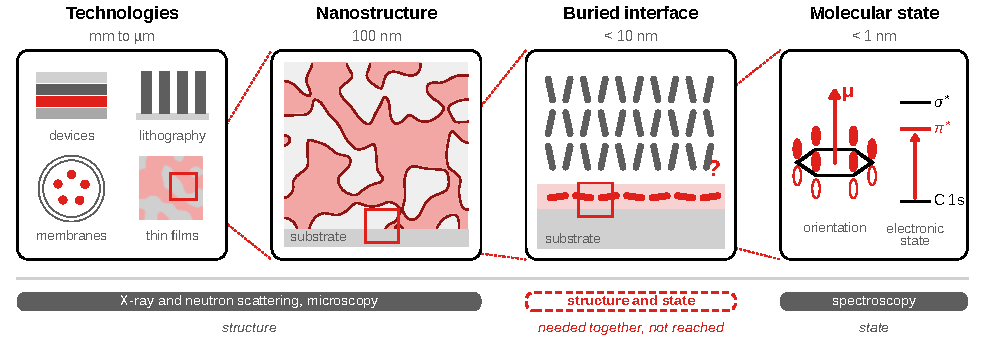
\includegraphics[width=\linewidth,height=0.75\textheight,keepaspectratio]{hero/hero_fig1-01_scales}
  \caption[From technologies to the molecular state of a buried interface.]{From technologies to the molecular state of a buried interface. Organic materials enter devices, lithographic patterns, membranes, and thin films at the millimeter to micrometer scale. Their function depends on nanostructure near \qty{100}{nm}, on the interfaces buried within that nanostructure below \qty{10}{nm}, and on the orientation and electronic state of the molecules that form those interfaces below \qty{1}{nm}. The bar beneath marks the reach of conventional measurements. X-ray and neutron scattering and microscopy resolve structure, spectroscopy resolves electronic state, and a buried interface requires both at once (red dashed box).}
  \label{fig:1.1}
\end{figure}


\section{Resonant Scattering}\label{sec:resonant-scattering}

Resonant soft X-ray scattering (RSoXS) uses incident photon energy as a mechanism for contrast variation so that by changing energy the otherwise hidden molecular state gradients can be revealed.\autocite{grabner2025resonant} At energies near the ionization energy of core atomic electrons (1s, 2s, 2p, etc.) the bonding configurations between molecules produce a rich series of transitions into unoccupied molecular orbitals leading to the near edge X-ray absorption fine structure (NEXAFS).\autocite{stohr2010nexafs} \Cref{fig:2.4} shows an example of the NEXAFS differences between three polymer components. By tuning photon energies around these resonant differences, RSoXS reveals scattering differences dictated by the underlying quantum transitions.

This mechanism provides RSoXS with sensitivity to the chemical gradients within nanostructures that are otherwise missed by traditional scattering. Because of this, RSoXS characterization has been instrumental to the organic device and polymer physics community to unravel hidden nanostructures formed by the mixing properties of polymers that are otherwise unresolved by neutron and X-ray techniques. Critically, this technique is not limited to simple transmission scattering approaches but has seen wide utility across geometries including reflectivity and diffraction revealing chemical composition in otherwise inaccessible interfaces.

Chemical composition is only one mode of the chemical state, the molecular orientation and packing statistics are also critically relevant to emergent function, most notably dictating charge transport between molecules in electronic device applications. In conjugated materials the overlap of π orbitals between neighboring molecules sets the electronic coupling along each direction, so the same material transports charge efficiently in the film plane when its molecules stand edge-on and between stacked electrodes when they lie face-on.\autocite{sirringhaus1999two} In light-emitting diodes the orientation of the emitting transition dipoles likewise sets the fraction of generated light that escapes the device.\autocite{yokoyama2011molecular} This anisotropy leaves a fingerprint in the polarization dependence of the optical response itself, since the transition dipole moments responsible for each resonant feature couple most strongly to light polarized along their own orientation, the central idea developed in \cref{chap:molecular-films}.

\section{A Short History of Resonant Soft X-ray Characterization}\label{sec:a-short-history-of-resonant-soft-x-ray-characterization}

Resonant contrast in the soft X-ray range was first exploited for orientation rather than structure. Near edge X-ray absorption fine structure spectroscopy matured during the 1980s as a probe of molecules adsorbed on surfaces, where the polarization dependence of each resonance places the corresponding bond relative to the substrate.\autocite{stohr2010nexafs} Because the carbon, nitrogen, and oxygen K edges all lie in the soft X-ray range, the same measurement distinguishes chemical moieties in organic materials that are nearly indistinguishable to hard X-rays, and standardized methods for carbon K-edge spectroscopy of polymers and organic films followed.\autocite{watts2006methods} Scanning transmission X-ray microscopy at third-generation synchrotron sources\autocite{bilderback2005review} brought this chemical and orientational sensitivity into real space with resolution well below \qty{100}{nm},\autocite{kilcoyne2003interferometer,ade2008nexafs} and undulators delivering variable linear polarization made the polarization direction an experimental variable in its own right.\autocite{young2002variable} Resonant scattering developed in parallel at the transition metal L edges, where the magnetic contrast of 2p resonances resolved chiral magnetic domains in ultrathin films\autocite{durr1999chiral} and the resonant magneto-optical constants needed to interpret such measurements were measured directly.\autocite{kortright2000resonant} These two lines of development, chemically specific spectroscopy of organic matter and resonant scattering as a structural probe, met at the carbon K edge.

Carbon K-edge resonant scattering followed in 2006, when the first transmission RSoXS measurements at the Advanced Light Source resolved polymer nanoparticles in a chemically similar matrix without staining or labeling.\autocite{araki2006resonant,mitchell2006molecular} A dedicated instrument at beamline 11.0.1.2 followed in 2010 and, with real-time data processing, opened the technique to a broad user community. Over the following years RSoXS became the standard measure of domain size and domain purity in organic photovoltaic blends, and established quantitative correlations between scattering-derived morphology and device efficiency.\autocite{yan2012correlating,jiao2017quantitative} In 2012, Collins et al. showed that polarized RSoXS is sensitive to the local orientation of molecules through their transition dipole moments, revealing non-crystalline orientational order in organic solar cell blends.\autocite{collins2012polarized} Tumbleston et al. then correlated this interfacial orientation with device performance.\autocite{tumbleston2014influence} Polarization-dependent scattering from organic films has since been traced to the optical anisotropy of the constituent molecules.\autocite{gann2016origins}

The technique has since spread well beyond organic photovoltaics and beyond the carbon edge. A second dedicated facility for polarized RSoXS operates at NSLS-II\autocite{gann2021nist}, and measurements at the nitrogen K edge and at the tender sulfur K edge reach heteroatoms that carbon contrast cannot isolate\autocite{zhong2022decoupling,freychet2021resonant,mcneill2023resonant}. Applications now include the helical and cubic phases of liquid crystals\autocite{salamonczyk2017structure,cao2020deciphering,cao2020molecular}, proteins and plant cell walls\autocite{ye2018resonant,ye2018resonanta,rongpipi2021resonant}, the latent images of lithographic resists\autocite{freychet2019reconstructing,zhang2024characterization}, and in situ and operando studies of solutions and electrochemical interfaces\autocite{zhong2021probing,yang2022textless,grabner2024molecular}. GPU-accelerated simulation of polarized scattering from three-dimensional morphologies now allows such measurements to be modeled directly\autocite{saurabh2023textless}. Across this range, the interpretation of every measurement rests on the optical constants assumed for each component, the dependence examined in the remainder of this chapter.

\section{Resonant Soft X-ray Reflectivity}\label{sec:resonant-soft-x-ray-reflectivity}

Specular reflectivity measures the depth profile of the refractive index rather than its lateral structure. Parratt's recursion for the reflected amplitude of a stratified medium remains the basis of its analysis\autocite{parratt1954surface}, with interfacial roughness entering through the Névot-Croce factor\autocite{nevot1980caracterisation} and anisotropic layers treated exactly by 4 × 4 transfer matrix formalisms.\autocite{berreman1972optics,yeh1980optics,passler2017generalized} At hard X-ray energies, however, the indices of low-Z organic layers differ too little for their interfaces to be resolved. Wang, Araki and Ade showed that tuning to the carbon K edge restores this contrast\autocite{wang2005soft}, and resonant soft X-ray reflectivity was soon applied to buried interfaces in organic light emitting diodes and other organic devices\autocite{wang2008multilayer,hexemer2007d} and to molecular orientation in soft matter films.\autocite{mezger2011molecular} Dichroic resonant reflectivity of ultrathin anisotropic organic layers and of an organic single crystal then showed that the anisotropic optical constants of an organic film can be determined quantitatively from reflectivity alone,\autocite{capelli2019quantitative,pasquali2014structural,capelli2016quantitative} and resonant reflectometry has recovered site-selective spectra with depth resolution\autocite{hamannborrero2017site}.

Polarization adds orientation to this depth sensitivity. The optical tensor of an oriented molecular film is anisotropic, so s- and p-polarized reflectivity weight its in-plane and out-of-plane components differently, so that the depth profile of orientation can be resolved together with that of composition. Thelen et al. used polarized resonant reflectivity to measure orientation depth profiles in vapor-deposited organic glasses, and Ferron et al. resolved the orientation and conformation of molecules at the buried heterointerfaces of vapor-deposited films.\autocite{ferron2023composition,thelen2020molecular,ferron2022characterization} Each of these studies treats the optical constants as inputs, either tabulated from NEXAFS of a reference film or fit freely at each energy, with Kramers-Kronig consistency imposed as a constraint only when the energy sampling is dense enough to support it.\autocite{kuzmenko2005kramerskronig,stone2012kramers} The depth profile is then only as reliable as these optical constants, which is the limitation this work addresses.

\section{Optical Models and Their Limits}\label{sec:optical-models-and-their-limits}

Interpreting RSoXS requires the optical tensor of the material at every measured energy, the complex index of refraction \(n = 1 - \delta + i\beta\), whose dispersive part \(\delta\) sets the phase of the transmitted and scattered waves and whose absorptive part \(\beta\) sets their attenuation. Most approaches measure \(\beta(E)\) across the absorption edge by NEXAFS, recover \(\delta(E)\) through the Kramers-Kronig relations\autocite{yan2013accurate,watts2014calculation}, and assign each resonance to a molecular orbital and its transition dipole moment so that angle-resolved NEXAFS fixes the orientation dependence of the tensor.\autocite{stohr2010nexafs} This works when resonances trace cleanly to bonds of known dipole orientation, as for the π* transitions of planar aromatic rings. For the polymer N2200, however, Gann et al. showed that angle-resolved NEXAFS cannot trace the absorption features of a large, conjugated repeat unit to individual moieties.\autocite{gann2014near} Density functional theory supplies the missing assignment in principle, yet calculations routinely return thousands of transitions, place them on an absolute energy scale with an offset, broaden them by an imposed rather than computed width, and treat an isolated molecule, so they have reproduced measured spectra only qualitatively.\autocite{su2017first} Murcia developed a clustering approach that reduces a DFT calculation to a handful of principal transitions and refines them against measured spectra, reproducing the NEXAFS of phthalocyanines quantitatively while retaining the transition dipole of each cluster.\autocite{murcia2026quantitative} This dissertation builds directly on that framework.

Most work in RSoXS rests solely on this idea of contrast variation, choosing energies and polarizations that maximize contrast between pre tabulated species offering only qualitative insights into the chemical states in buried structures and at heterointerfaces. This presupposes that the potential molecules within these structures come from a set of pre characterized molecules that have been measured independently ahead of time. The natural consequence of this comes a lack of specificity against hydrocarbon contaminants and oxidations that may share similar spectral characteristics to the hypothesized compound family but deviate strongly outside of the few measurement energies. It is therefore never possible to exclude or characterize these contaminants. Similarly, at interfaces if novel molecular conformations or hybridization impact the optical response uniquely, then these characteristics cannot be uncovered. What is needed to resolve this is the full spectral measurement, collecting RSoXS across an entire absorption edge and with multiple polarizations. However, successfully analyzing this data requires a framework to produce accurate and facile anisotropic optical tensors that describe the energy and polarization dependence of the optical response, and are directly interpretable to uncover the molecular states responsible for this emergent response.

\section{Scientific Questions and Hypotheses}\label{sec:scientific-questions-and-hypotheses}

The framework called for above must supply an anisotropic optical tensor for every layer of a film at every energy and polarization. The reflectivity studies reviewed earlier obtain that tensor in one of two ways, tabulated beforehand from NEXAFS of a reference film and held fixed, or fit freely at each measured energy, with Kramers-Kronig consistency imposed only when the energy sampling is dense enough to support it. The first practice rests on the presumption that the molecules in every layer are the reference in some orientation and density, so a layer that departs from the reference can be neither interpreted nor explained. The second rests on no presumption about the molecule, so nothing about the molecule follows from it without a secondary analysis, and its parameter count grows with every energy added. One question is asked of each practice. The first concerns what becomes measurable when the tabulated tensor is replaced by one derived from the electronic structure of the molecule. The second concerns how the physical constraints that make such a derivation possible can be carried into the recovery of a tensor that no reference supplies, with the answer to the second resting on what the first establishes.

Murcia's clustering reduces a DFT calculation, which returns far more transitions than any spectrum resolves, to the few principal transitions that reproduce a measured NEXAFS spectrum once their strengths and widths are refined against it, with each retained cluster keeping the transition dipole assigned to it by the calculation. The tensor of a film is the ensemble average of that single-molecule response over the orientations and packing of the molecules within it, so the projection of each dipole through the orientation distribution of a layer gives the full energy and polarization dependence of that layer from its molecular tilt and density alone. The construction is not yet an analysis. The refinement is carried out against angle-resolved NEXAFS of a reference film whose own orientation enters the measured dichroism, so the dipole direction of each cluster and the tilt of the molecule are entangled in the same data used to fix both, and the clustering retains only the transitions selected as principal, so a weak, misassigned, or absent transition enters the tensor as an error present at every depth. Whether a tensor built this way can support a polarized resonant soft X-ray scattering analysis, and what such an analysis returns that the tabulated tensor cannot, is the first question of this work. \emph{\textbf{How can an optical tensor derived from ML-refined DFT be built into the analysis of resonant soft X-ray scattering, and what does that integration make measurable about the molecular state of a buried interface?}}

Much of what the integration would give can be reasoned out before it is attempted. With the spectral response fixed by the molecule, a layer is specified by its order and density, so the number of parameters no longer depends on how many energies are measured, and each added energy tightens the constraint on the same few parameters where it previously added its own set of tensor components to be fit. Because those parameters set the amplitude and phase of the reflectivity fringes at every energy and polarization, the energies that free fits treat as independent experiments become one overdetermined measurement of structure, with the thickness and sharpness of an interfacial layer constrained by how the fringes change across the edge in addition to their spacing at any one energy, so the features such a fit resolves need not be larger than the diffraction limit set by the largest momentum transfer measured. The dichroism of every resonance follows from the dipoles and the tilt, so the polarization dependence that a free fit absorbs into separate in-plane and out-of-plane components becomes a prediction. Because the tensor admits only the molecule, a fit can fail. A free tensor accommodates any layer, so a surface or buried layer whose optical constants differ from the bulk can be assigned to contamination or oxidation without that assignment ever being tested, whereas a tensor fixed to the molecule either reproduces such a layer with a different tilt and density or does not reproduce it, with the residual at the molecule's own resonances distinguishing the two.

What cannot be reasoned out in advance is how a wrong tensor behaves in a fit. A cluster carrying the wrong dipole, or a transition that the reference film did not contain, might appear as misfit at particular energies, or it might be absorbed into whichever structural parameters are free, biasing the recovered profile while the fit appears sound. The two cases can be separated only by fitting the same data with both tensors, a comparison that serves as the test of the first hypothesis. We hypothesize that existing reflectivity measurements contain more about the molecular state at buried interfaces than free-tensor analyses return, with a tensor derived from the molecule recovering that information and resolving order and density below the diffraction limit from fewer parameters and with smaller uncertainties than the free tensor requires. If the hypothesis holds, with a tensor that admits only the molecule reproducing the layers that free fits attribute to contamination, those layers become the molecule in another state, and the profile of orientation and density returned by the fit, together with the account of film growth read from it, becomes a product of this question, discussed where it arises without directing the work. If the hypothesis fails, the failure is itself informative, since the misfit then falls at the energies where the reference film and the buried molecules differ.

The premise of the first question is that the molecules in the film are the molecule of the reference. At an interface that premise can fail, since packing, conformation, and hybridization with a neighbor alter the unoccupied orbitals into which the core electron is excited. For species that cannot be prepared as standards, such as volatile solvents or molecules in conformations that occur only at an interface, it fails outright. The tensor must then be recovered from the scattering itself. Fitting it energy by energy restores the parameter explosion and discards a constraint that the physics supplies, since nothing in such a fit requires the optical constants found at one energy to be consistent with those found at another. The Kramers-Kronig relations tie the dispersion at every energy to the absorption at every other, so the dispersion below the edge, which sets the critical angles that anchor every reflectivity profile, is determined by the absorption across the whole edge. Nothing prevents optical constants fit independently from violating these relations, so such a fit can return dispersion that no causal medium could produce, with the violation undetectable short of sampling the entire edge. Any recovery of optical constants from scattering must therefore impose causality. Kuzmenko's variational analysis does so by expanding the optical response in Kramers-Kronig consistent basis functions, an approach that the triangle basis of Stone et al. has carried to resonant reflectivity across a full absorption edge, but each measured energy gains a basis function, so the dense sampling the method requires returns the parameter growth it was meant to remove. The alternative follows from the first question. The ML-DFT clusters are already a set of transitions at known energies with known dipoles. Written as oscillators whose line shapes carry their own Kramers-Kronig conjugates, they form a basis that is causal by construction, anisotropic through its dipoles, and fixed in size by the number of transitions in the molecule rather than the number of energies in the measurement. \emph{\textbf{How can the optical constants of a buried molecular state be recovered from the scattering itself, under the same physical constraints that made the first analysis possible, and what do they reveal about the electronic states that molecules adopt at an interface?}}

With such a basis the gains of the first question carry over. The parameter count is set by the number of resonances, so the strength of each resonance can be refined as a function of depth, and the orientation of its dipole separately from the molecular tilt, without the fit becoming underdetermined. The anisotropy of a buried layer then becomes a measured quantity, and because every trial spectrum is causal, no fit can return optical constants that a real medium could not possess. Reflectivity then returns a spectrum localized to a region that no reference measurement can isolate, a depth-resolved spectroscopy whose parameters trace back to families of electronic transitions. The interfacial states found under the first question, together with the observation that NEXAFS of films prepared under nominally identical conditions differs, leave open whether molecules within a monolayer of an interface occupy electronic states that differ from the bulk, with the oscillator basis allowing that question to be put to the data resonance by resonance. The measurement itself raises a second question, since exact optical constants at a few energies leave the spectrum between them unconstrained, so the choice between a few precisely measured energies and a continuous scan across the edge, settled so far by convention and by the cost of beamtime, acquires a quantitative answer. We hypothesize that an oscillator basis tied to transition dipoles allows the optical response of a buried region to be refined together with the structure, with the molecules at an interface differing from the bulk in the strengths of particular transitions, in ways that no rescaling of a reference spectrum reproduces, and with the spectrum recovered from a sparse measurement limited by how the edge is sampled before it is limited by the precision at any one energy. These claims are tested in Alq\textsubscript{3} and ZnPc against fits that hold a measured NEXAFS spectrum fixed, and on synthetic spectra sampled by several strategies. The limit in which no calculation supplies the transitions, and only their number is assumed, is discussed but remains to be tested on a measured interface.

Both questions rest on measured NEXAFS, from which the clusters are refined and against which recovered spectra are judged, yet spectra of nominally identical films differ. A spectrum must therefore be judged before it is reused, which requires that the raw measurement stay linked to every optical constant derived from it, that spectra from different beamlines share one normalization and processing convention, that quality be scored by reproducible metrics, and that every result carry its provenance under a versioned and citable identifier that analysis pipelines can reach programmatically. X-ray Atlas is built to these requirements, as the infrastructure both questions assume, with no question of its own.

\section{Overview}\label{sec:overview}

This work presents the development of facile anisotropic optical tensor models that directly connect the emergent response to both the physical molecular state and the electronic states within the molecules. Each resonant feature is traced to the family of electronic transitions that produces it. This builds on the developments of Dr. Victor Murcia's Ph.D. dissertation, which used machine learning to integrate density functional theory calculations of electronic states with experimental measurements of absorption spectroscopy.\autocite{murcia2026quantitative} Through this framework each resonant feature can be described by a handful of transitions, each bearing a transition dipole moment that describes its anisotropic response. This isolates the single molecule optical response so that each molecular assembly can be constructed from the correct ensemble averaging of the molecular populations within it, allowing the direct measurement of properties such as molecular orientation and packing without a secondary analysis. Applying this to RSoXS in reflection geometry constrains the molecular state evolution far below the nominal diffraction limit.

Because each cluster carries its own oscillator strength and transition dipole, the resonances themselves become quantities that can be tracked through a film. Where the molecular state at a heterointerface alters the electronic structure, through a new conformation, hybridization with a neighbor, or a change in packing, the amplitudes and dipole orientations of the affected resonances change with depth while the others do not. Refining them as functions of depth recovers a spectrum localized to regions that no reference measurement can isolate, such as a buried interface a single molecular layer thick. This approach, developed in \cref{chap:resonances}, extends resonant reflectivity from contrast variation to depth-resolved spectroscopy.

Finally, this dissertation presents a modern platform for collaborative open data surrounding anisotropic optical tensors. Programmatic, standardized access to reusable optical models for molecular materials is critical to tracing the molecular evolutions within a film. Present best practices make data `available upon request', yet this denies the programmatic access that cross-publication meta-analyses require, leaving unexamined the phenomena that each analysis misses on its own. This part of the work is a collaboration among seven institutions in three countries.

The remainder of this dissertation is organized around these questions. \Cref{chap:molecular-films} sets out the materials and optical background of the work. It describes the device properties that molecular packing controls, the growth of vapor-deposited ZnPc and Alq\textsubscript{3} films and the open problems of their first molecular layer, the core excitations that give each resonance a transition dipole and the contrast it produces, the oscillator and Kramers-Kronig relations that turn those resonances into optical constants, and the DFT calculations, clustering, and refinement that supply the resonances of each molecule. It closes by projecting the refined molecular tensor into the frame of a film and testing a film of uniform tilt against angle-resolved NEXAFS of ZnPc. \Cref{chap:methods} contains the fundamentals and methods of polarized resonant soft X-ray reflectivity used throughout. Far-field scattering is recast around the specular geometry, with the reason that specular reflectivity cannot be treated kinematically made explicit, and the orientation-gradient profile used in \cref{chap:znpc} is derived. The measurement at ALS beamline 11.0.1.2 is described from sample alignment through scan configuration, reduction, stitching, and the uncertainty budget. The analysis methods cover the exact transfer matrix calculation for stratified anisotropic media, the interfacial roughness models, objective transforms, optimizers, posterior estimation, and model selection, with Bayesian optimization and amortized inference presented as the route to autonomous measurement.

In \cref{chap:znpc}, which reproduces the ZnPc manuscript, the first question is put to vapor-deposited ZnPc films on native-oxide silicon. The single-molecule tensor is constructed from DFT transition clusters refined against angle-resolved NEXAFS of an edge-on film, and the film is modeled first as three slabs, each described by a density and a molecular tilt, against the conventional alternative in which the uniaxial tensor components are fit freely at every energy in every slab. The ML-DFT tensor reproduces the reflectivity across the pre-edge and the resonance series with equal or smaller residuals from an order of magnitude fewer parameters, with correspondingly smaller uncertainties. Because the tensor admits only ZnPc, the contamination or oxidation customarily assigned to interfacial layers is not required by the data within the sensitivity of the resonance series. The slab structure is then replaced by a single continuous profile in which orientation and density relax from a pinned state at each interface into the bulk over a characteristic length. This profile fits better with fewer parameters still, and with it a face-on, lower-density state is resolved within one molecular layer of the oxide, along with a denser state oriented near the magic angle at the free surface, both finer than the diffraction limit. These profiles are read against substrate patterning and against a growth front on which substrate adhesion competes with π-π cohesion, with the consequence that coverage-checkpoint studies record a transient state of the growth front rather than the buried interface of a continuously deposited film.

In \cref{chap:resonances} the second question is put to two systems. The optical response is written as a sum of Kramers-Kronig consistent oscillator pairs, each a Gaussian absorption with its Dawson-function conjugate, tied to the ML-DFT transition clusters so that every oscillator carries a transition energy, a width, an oscillator strength, and a dipole orientation from which the tensor follows. For Alq\textsubscript{3}, whose NEXAFS differs between films prepared under nominally identical conditions, the amplitudes of the principal resonances are refined with depth, removing a degeneracy between the optical model and the film density that a borrowed spectrum can resolve only by driving the substrate density to an unphysical value. For the ZnPc films of \cref{chap:znpc}, the amplitude and dipole cone angle of each principal π* resonance are refined and compared with the conventional NEXAFS-fixed tensor, with the improvement concentrated at the energies of strongest orientation sensitivity and with the two lowest resonances exchanging oscillator strength between the free surface and the oxide interface. A synthetic carbon edge of known transitions is then used to compare sampling strategies, energies placed on the resonances, drawn at random, or chosen by a Gaussian-process design, against a continuous scan with larger noise at each point. Sparse measurements are found to be limited by the number and placement of energies before they are limited by the precision at any one of them. The same construction serves as a generator of Kramers-Kronig consistent optical constants for planning measurements.

\Cref{chap:xray-atlas} presents X-ray Atlas, an open and programmatic database of NEXAFS spectra and of the optical constants and versioned optical models derived from them, built around the provenance, quality metrics, and citable identifiers that reuse requires. The data model links each raw measurement to its processed spectrum and derived optical constants, every contribution is normalized under one server-side convention and scored by fixed metrics of energy resolution, signal to noise, and normalization residual, contributors are identified through ORCID, and each processing revision receives a persistent DOI. A REST interface, a Python package, and a command-line client extend the same records to scripted analysis. Optical models pin a dataset revision, so a tensor such as the one of \cref{chap:znpc} can be forked, cited, and reproduced. The answers to both questions are collected in \cref{chap:conclusion}, together with the extensions they open, finite element and neural surrogate solvers for geometries without an exact layered solution, the oscillator description applied to polymers and other absorption edges, and autonomous measurement at the beamline.

\chapter{Molecular Films and Their Resonant Optical Response}\label{chap:molecular-films}

This chapter sets out the materials science and the optical physics on which the later chapters rest. It begins with the device properties that molecular packing controls and with the growth of vapor-deposited films of the two molecules studied here, ZnPc and Alq\textsubscript{3}. It then treats a single C 1s excitation. The orbitals of a conjugated bond fix the direction of its transition dipole and with it the contrast the resonance produces, a driven oscillator built on that dipole yields a causal pair of optical constants, and DFT calculations reduced by clustering supply the oscillators of a whole molecule. The chapter closes by projecting the refined molecular tensor into the frame of a film and testing a film of uniform tilt against angle-resolved NEXAFS of ZnPc.

\section{Packing and the Emergent Properties of Molecular Films}\label{sec:packing-and-the-emergent-properties-of-molecular-films}

\begin{figure}[htp]
  \centering
  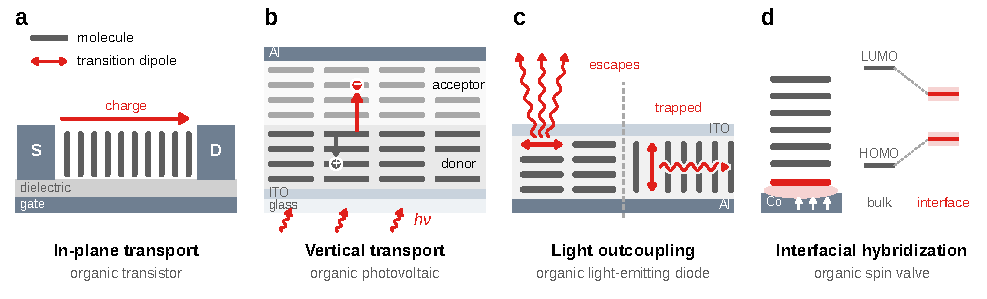
\includegraphics[width=\linewidth,height=0.75\textheight,keepaspectratio]{hero/hero_fig2-01_packing}
  \caption[Molecular orientation sets the function of organic devices.]{Molecular orientation sets the function of organic devices. Molecules are drawn as slabs seen edge-on and transition dipoles as red arrows. (a) Organic transistor, in which molecules standing edge-on between source (S) and drain (D) stack their π systems along the channel and carry charge in the plane of the film. (b) Bilayer organic photovoltaic with face-on donor and acceptor layers between ITO and Al. Light entering through the glass is absorbed in the donor, and charge separates at the heterointerface, the electron passing into the acceptor and the hole returning through the donor. (c) Organic light-emitting diode. Emitters lying flat carry in-plane dipoles whose light escapes through the ITO (left), while upright emitters radiate along the film and their light remains trapped in the stack (right). (d) Organic spin valve, in which the first molecular layer on the Co electrode (red) hybridizes with the metal, shifting and broadening its HOMO and LUMO relative to the bulk film. The property set by orientation and a representative device are named beneath each panel.}
  \label{fig:2.1}
\end{figure}

Conjugated molecules interact with their neighbors through the overlap of their π orbitals, and the overlap depends on how the molecules are arranged. The electronic coupling between two molecules falls off steeply with their separation and with the angle between their π systems, so a film of identical molecules can conduct well along one direction and poorly along another.\autocite{bredas2004charge} In a planar molecule such as ZnPc the π orbitals stand normal to the molecular plane, so the strongest coupling runs along the stacking direction between cofacial neighbors and the coupling between neighbors that meet edge to edge is weak. The optical transitions of such a molecule are anisotropic as well, since its π to π* transitions have their dipoles in the molecular plane. The molecule absorbs and emits light polarized in that plane and absorbs light polarized along its normal only weakly, the reverse of the C 1s to π* excitations treated later in this chapter, whose dipoles stand normal to the plane. Nearly every property of a molecular film that matters in a device is anisotropic in this way, and the direction in which each property is large is set by the orientation of the molecules relative to the electrodes and interfaces around them. A molecule lying face-on, with its plane parallel to the substrate, stacks its π systems through the thickness of the film and lays its optical transition dipoles in the plane of the film. A molecule standing edge-on, with its plane perpendicular to the substrate, stacks its π systems within the plane of the film and turns part of its optical response toward the film normal. \Cref{fig:2.1} shows four classes of device in which this dependence is decisive, and no single orientation serves all four.

In a field-effect transistor charge moves between source and drain electrodes that lie in the plane of the film (\cref{fig:2.1}a). Molecules standing edge-on to the dielectric stack their π systems along the channel, and polymer films with this orientation reach mobilities about two orders of magnitude higher than films of the same polymer lying flat.\autocite{sirringhaus1999two} Face-on molecules in the same channel pass charge between neighbors only through the weak coupling of molecules that meet edge to edge, or across the boundaries between domains of different orientation. The current flows in the first few molecular layers above the dielectric\autocite{dodabalapur1995organic}, so the orientation at a buried interface sets device performance.\autocite{dindault2022correlating} The gate field draws the accumulated charge against the dielectric and holds it there, so a film whose bulk is well ordered can still perform poorly when its first layer adopts a different orientation, packs less densely, or breaks into small domains.

A photovoltaic cell requires the opposite arrangement (\cref{fig:2.1}b). Light enters through a transparent electrode, excitons form in the donor, and charge separates at the donor-acceptor heterointerface before it travels through the thickness of the film to the electrodes. Face-on molecules stack their π systems along that path and lay their transition dipoles in the plane of the film, parallel to the electric field of light arriving along the normal, so they absorb that light more strongly than edge-on molecules, which present only part of their transition dipole to the field. Charge separation and recombination both proceed by electron transfer between donor and acceptor molecules in contact. The coupling for that transfer depends on the overlap of the two π systems in the same way as the coupling between like molecules, so the relative orientation of donor and acceptor sets the balance between separation and recombination. At the heterointerface itself, face-on orientation of the donor relative to the acceptor raises the yield of separated charge, and the performance of polymer solar cells follows the orientation of the molecules at that interface more closely than the orientation in either bulk layer.\autocite{tumbleston2014influence}

In a light-emitting diode the orientation of the emitting dipoles sets the fraction of the generated light that leaves the device (\cref{fig:2.1}c). Light generated in the organic layers, whose refractive index exceeds those of the glass substrate and of air, escapes only within a narrow cone about the film normal, and light outside that cone is totally reflected at the substrate and air interfaces. A dipole radiates most strongly perpendicular to its own axis, so an emitter whose dipole lies in the plane of the film sends its light toward the viewer, while an emitter whose dipole stands along the film normal sends its light along the film, where it remains trapped in waveguided and surface plasmon modes. For an emitter whose transition dipole lies in the molecular plane, face-on molecules contribute only horizontal dipoles and edge-on molecules contribute vertical components as well, so the fraction of light that escapes follows the distribution of molecular orientation in the emitting layer. Such a preferred orientation can form even in the amorphous films used as emitting layers, which have no crystalline order. Horizontal alignment of the emitters raises the fraction of light that escapes by roughly half relative to an isotropic film.\autocite{yokoyama2011molecular,brutting2013device}

In an organic spin valve the relevant property is the electronic state of the molecules in contact with a ferromagnetic electrode (\cref{fig:2.1}d). The device passes current from one ferromagnetic electrode through the molecular layer to a second, and its resistance changes when the relative magnetization of the two electrodes is reversed, provided the carriers retain a net spin polarization across the layer. Molecules in that first layer hybridize with the metal, which shifts and broadens their frontier orbitals and can polarize them in spin, so the interface acts as a spin filter with properties of its own. The majority and minority spin states of the ferromagnet couple to the molecular orbitals with different strengths, so the interfacial layer can enhance the spin polarization of the injected current or reverse its sign relative to that of the bare electrode.\autocite{sanvito2010rise,barraud2010unravelling} The strength of this coupling depends on the overlap between the molecular orbitals and the metal states, which is largest when the π system lies flat against the electrode and decreases with the height at which the molecule sits, so the spin filtering of the interface follows the orientation and adsorption height of its first molecular layer. The same interaction sets the alignment of energy levels at every metal-organic contact. Charge transfer between molecule and metal and the redistribution of metal electrons beneath the adsorbed layer form an interface dipole that shifts the molecular levels away from the positions predicted by aligning the vacuum levels of the two materials, and with them the barrier to charge injection in each of the devices above.\autocite{ishii1999energy}

Orientation specifies how a rigid molecule sits, yet a molecule at an interface also has internal degrees of freedom, and the conformation it adopts there need not match the one it adopts in the bulk. Torsions between linked rings, the arrangement of ligands about a metal center, and the planarity of a macrocycle all respond to the forces at an interface. A molecule bound to a reactive surface can bend or twist to bring more of its π system into contact, a molecule confined between a substrate and the layer above can be flattened, and a metal complex whose central atom meets the substrate on one face can shift its ligands to accommodate the contact. Even a rigid macrocycle such as ZnPc can in principle bend out of plane when its central ion or its outer rings bind to a substrate, and the quinolinolate ligands of Alq\textsubscript{3}, described in the next section, have more freedom still. Each change alters the overlap of the π system with itself and with the material beneath it, and with it the energies of the frontier orbitals, the strength of hybridization with the substrate, and the directions of the transition dipoles that govern absorption and emission.

Changes of this kind could give an interface properties found in neither the substrate nor the bulk film. A torsion that interrupts the conjugation of a molecule would localize its frontier orbitals and weaken its coupling to neighbors, a distortion that lowers the symmetry of a molecule would split degenerate orbitals and allow transitions that are forbidden in the free molecule, and a change in the bonding at a metal center would alter both the injection barrier and the spin-dependent hybridization described above. Whether such states form at the buried interfaces of working films, and how strongly they matter, has not been established, because no available measurement resolves the conformation of a single molecular layer beneath a film. Diffraction records the periodic packing of crystalline grains averaged through the film, photoemission and scanning probes reach exposed surfaces and submonolayer coverages, which continued deposition buries and can alter, and spectroscopies of the whole film average the interfacial layer with the many layers above it. Interfacial conformation therefore remains an open variable, likely minor in many systems but ruled out in none by present measurements. Its signature would appear in the resonances of the interfacial layer, since a change of conformation shifts the energies, strengths, and dipole directions of the transitions it involves, and the depth-resolved refinement of resonance amplitudes developed in \cref{chap:resonances} is sensitive to such changes even where it cannot identify their cause.

In all four devices the property of interest is set where molecules meet another material, a dielectric, an acceptor, an electrode, or a ferromagnet. At each of these interfaces the orientation, packing, and possibly the conformation of the first molecular layer set the coupling that matters, between molecules in a transistor channel, between donor and acceptor in a solar cell, between emitting dipoles and the optical modes of a diode, and between molecular orbitals and metal states at an electrode. The arrangement and electronic state of thosemolecules are also the quantities that conventional measurements reach least well, since they lie beneath the film and occupy one or two molecular layers. Resolving them requires a probe that reaches a layer of that thickness beneath a finished film and responds to both the orientation and the electronic structure of its molecules. The resonant optical response developed in the rest of this chapter is built for that purpose.

\begin{figure}
  \centering
  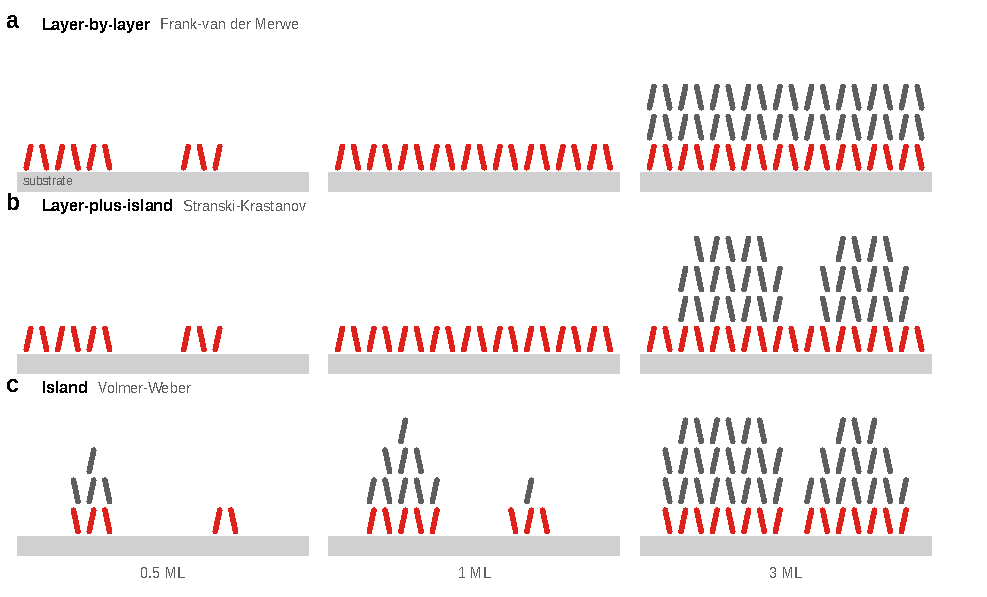
\includegraphics[width=\linewidth,height=0.75\textheight,keepaspectratio]{molecular-chapter/molch_growth}
  \caption[Growth modes of a vapor-deposited molecular film.]{Growth modes of a vapor-deposited molecular film. Standing molecules are drawn as slabs on a substrate at nominal coverages of 0.5, 1, and 3 monolayers (ML), with the molecules in contact with the substrate in red. (a) Layer-by-layer (Frank-van der Merwe) growth, in which each layer completes before the next nucleates. (b) Layer-plus-island (Stranski-Krastanov) growth, in which a complete wetting layer forms before three-dimensional islands nucleate on it. (c) Island (Volmer-Weber) growth, in which islands nucleate directly on the substrate and leave it partly exposed until they coalesce.}
  \label{fig:2.2}
\end{figure}

\section{Growth of Vapor-Deposited Molecular Films}\label{sec:growth-of-vapor-deposited-molecular-films}

The films studied here are grown by physical vapor deposition, in which molecules sublimed from a heated source condense on a substrate held in vacuum. The arrangement they adopt is set during growth by a competition between the attraction of each arriving molecule to the substrate and its attraction to the molecules already deposited.\autocite{venables1984nucleation,bauer1958phanomenologische} Three growth modes bound the possibilities (\cref{fig:2.2}). When adhesion to the substrate dominates, molecules spread into a complete layer before the next layer nucleates, the layer-by-layer or Frank-van der Merwe mode. When cohesion dominates, molecules gather into three-dimensional islands that leave the substrate exposed until the islands coalesce, the island or Volmer-Weber mode. Layer-plus-island or Stranski-Krastanov growth lies between the two, with a wetting layer that forms first and islands that grow on it.

Molecular films depart from this atomic picture in two ways that matter for the interface. A planar molecule binds to a substrate and to its neighbors with energies that depend on its orientation, so the competition between adhesion and cohesion selects an orientation as well as a growth mode.\autocite{forrest1997ultrathin,witte2004growth} Molecules lying flat maximize their contact with a strongly interacting substrate, molecules standing on edge maximize their π contact with one another, and the orientation adopted in the first layer need not persist once that layer is covered. Growth is also kinetic. The deposition rate and the substrate temperature set how far each molecule diffuses before it is buried, so the structure of a film can change with thickness, and its first layers can be trapped in states that would not form at equilibrium.\autocite{kowarik2008organic}

Zinc phthalocyanine (ZnPc) is the template for this discussion and for the measurements of \cref{chap:znpc,chap:resonances}. It is a planar, rigid macrocycle of \(D_{4h}\) symmetry in which four isoindole units surround a central zinc ion, and its carbon atoms fall into four inequivalent sites, each with its own core level (\cref{fig:4.1}). On native-oxide silicon ZnPc forms polycrystalline films in a herringbone packing with the molecules standing edge-on, while on templating layers such as CuI and graphene it adopts a brickstone packing with the molecules lying face-on.\autocite{kato2020morphological,ngongangndjawa2015impact,schunemann2011zinc} The templating picture assigns the orientation of the whole film to the first layer, much as a seed layer sets the orientation of an epitaxial inorganic film. Coverage-checkpoint studies, which interrupt deposition to measure a partial film, test this picture and disagree with one another. In situ measurements resolve a density stratification inconsistent with simple templating\autocite{derrien2022interfacial}, while other work argues that an exposed growth front records a transient state that changes once it is buried.\autocite{yamamoto2022variation,deoteyza2006structural}

Tris(8-hydroxyquinolinato)aluminum (Alq\textsubscript{3}), the second molecule studied here, shows why the electronic state of a molecule in a film cannot be assumed from its formula. Three quinolinolate ligands coordinate a central aluminum ion, each through one oxygen and one nitrogen, and the six donor atoms can take two arrangements. The meridional (mer) isomer places the three oxygens in one plane through the metal, and the facial (fac) isomer places them on one face of the coordination octahedron.\autocite{brinkmann2000correlation,colle2003preparation} Vapor-deposited films consist mainly of the mer isomer, are amorphous with weak orientational order, and leave the ligands some conformational freedom about the metal. Alq\textsubscript{3} was the emitter and electron transporter of the first efficient organic light-emitting diode\autocite{tang1987organic} and remains a standard molecule in studies of organic spin valves.\autocite{xiong2004giant,barraud2010unravelling} Its role in this work complements that of ZnPc. ZnPc tests whether orientation can be resolved at a buried interface, and Alq\textsubscript{3} tests whether the electronic state of a molecule, as recorded in its NEXAFS, is the same in every film. \Cref{chap:resonances} takes up that question without assigning the differences it finds to a particular cause.

Films of both molecules leave open where the first molecular layer sits and why, whether its orientation and density follow the substrate, follow the bulk, or take a form of their own. They also leave open whether molecules within a monolayer of an interface occupy electronic states that differ from those of the bulk, through hybridization with the substrate, a change of conformation, or a change of packing. Measurements of an exposed growth front cannot settle either problem, since continued deposition buries the interface and can alter it. Both require a measurement of orientation and electronic state at the buried interface of a finished film, which the rest of this chapter prepares optically and \cref{chap:znpc,chap:resonances} carry out.

\section{Core Excitations and Transition Dipoles}\label{sec:core-excitations-and-transition-dipoles}

\begin{figure}[htp]
  \centering
  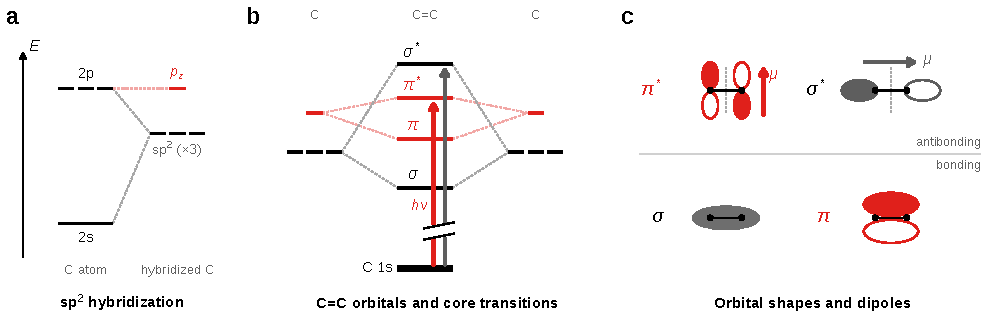
\includegraphics[width=\linewidth,height=0.75\textheight,keepaspectratio]{molecular-chapter/molch_orbitals}
  \caption[Orbitals and core transitions of a conjugated carbon bond.]{Orbitals and core transitions of a conjugated carbon bond. Energies are not to scale. (a) Mixing of the carbon 2s orbital with two 2p orbitals gives three sp2 hybrids, while the remaining pz orbital is unchanged. (b) Hybrids on two neighboring carbons form the σ and σ* orbitals of the C=C bond, and their pz orbitals form π and π*. Absorption of an X-ray photon promotes a C 1s electron into the empty π* (red) or σ* (gray) level. (c) Shapes of the four orbitals along the bond, with filled and open lobes of opposite phase, bonding orbitals below, antibonding orbitals above, and dashed lines at nodal planes. The transition dipole μ of C 1s → π* lies along the p orbitals, normal to the molecular plane, while the dipole of C 1s → σ* lies along the bond.}
  \label{fig:2.3}
\end{figure}

The resonances that give soft X-ray measurements their chemical and orientational sensitivity are excitations of a core electron into unoccupied molecular orbitals, and in a conjugated molecule those orbitals follow from the hybridization of carbon (\cref{fig:2.3}). The 2s orbital and two of the 2p orbitals of each carbon mix into three sp\(^{2}\) hybrids that lie in the molecular plane at \ang{120} to one another, and the remaining 2p orbital, \(p_{z}\), stands normal to that plane (\cref{fig:2.3}a). Hybrids on neighboring atoms overlap head-on to form the σ bonds of the molecular framework, and the \(p_{z}\) orbitals overlap side-on to form the delocalized π system (\cref{fig:2.3}b). Each overlap yields a bonding orbital, occupied in the ground state, and an antibonding orbital, empty in the ground state and available as the final state of an X-ray excitation.

Side-on overlap is weaker than head-on overlap, so the π pair is split less than the σ pair and the π* orbitals lie lowest among the empty states. The carbon K edge shows this ordering directly. Excitations from C 1s into π* orbitals give sharp resonances between about 284 and \qty{290}{eV}, and excitations into σ* orbitals, most of which lie above the ionization threshold and couple to the continuum, give broader resonances from about \qty{290}{eV} upward.\autocite{stohr2010nexafs} The C 1s orbital is confined to one atom and barely perturbed by bonding, so each excitation starts from a known site, and carbons in different chemical environments contribute resonances at different energies.

The absorption spectra are set by the coherent sum of electronic transitions excited by incident photons. For X-ray photons incident on molecular materials, the initial state is commonly an atomic orbital deep within the atomic potential well and minimally perturbed by the molecular bonds (\cref{fig:2.3}b). The final states, however, are delocalized unoccupied molecular orbitals that commonly stretch over a large portion of the molecule. Fermi's golden rule relates the transition dipole moment (TDM) between the initial and final states to the transition probability, i.e.,

\begin{equation}
  \Gamma_{ij} \propto \bigl|\langle f \,|\, \mathbf{\mu} \cdot \mathbf{E} \,|\, i \rangle\bigr|^{2},
  \label{eq:golden-rule}
\end{equation}

where \(\mathbf{\mu}\) is the dipole operator and \(\mathbf{E}\) the electric field of the incident photon. The oscillator strength of the transition, \(f_{if} \propto \omega_{fi}\,|\langle f \,|\, \widehat{\mathbf{e}} \cdot \mathbf{\mu} \,|\, i \rangle|^{2}\) with \(\widehat{\mathbf{e}}\) the unit polarization vector, sets the integrated absorption cross section of the corresponding resonance and therefore its area in the absorption spectrum.\autocite{stohr2010nexafs} \Cref{chap:resonances} tracks this quantity for individual resonances. Because the transition probability depends on the alignment between the polarization and the transition dipole, the absorption is a tensor quantity. In scattering this appears as a polarization-dependent contrast tied to molecular orientation and to the bonding conformations that set the relative orientation of the transition dipoles within the film.

The direction of each transition dipole follows from the shape of the final orbital (\cref{fig:2.3}c). The C 1s orbital is spherical, so the dipole operator connects it only to the p character of the final state on the excited atom, and the transition dipole points along that p component. For a π* final state, built from \(p_{z}\) orbitals, the dipole lies along the normal to the molecular plane. For a σ* final state, built from hybrids directed along a bond, the dipole lies along that bond and therefore in the molecular plane. Every resonance of a planar conjugated molecule thus carries a direction fixed in the frame of the molecule, and its absorption scales as the squared projection of the electric field on that direction.

\section{Chemical and Orientational Contrast}\label{sec:chemical-and-orientational-contrast}

\begin{figure}[htp]
  \centering
  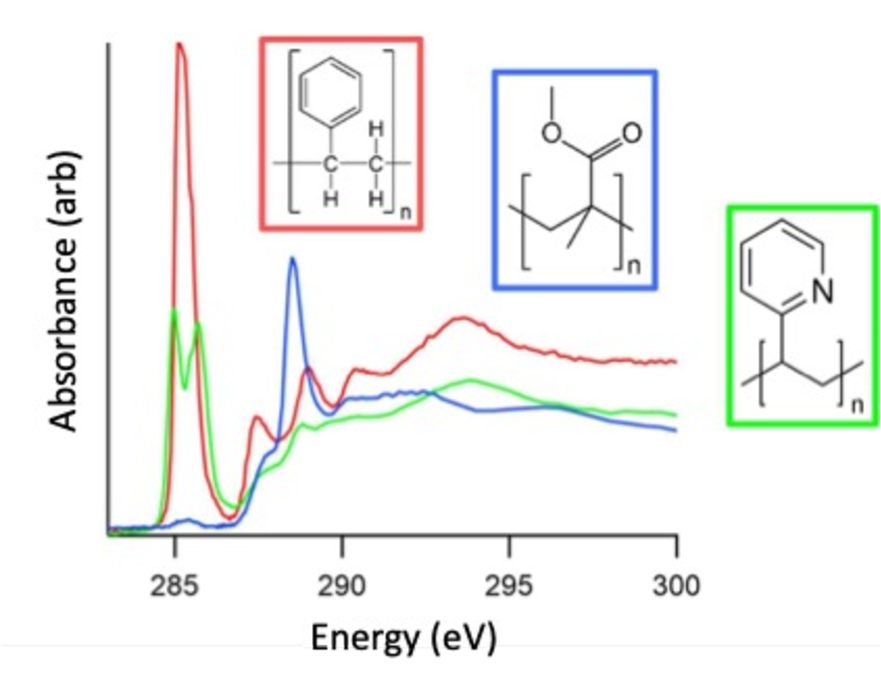
\includegraphics[width=0.6\linewidth,height=0.75\textheight,keepaspectratio]{fig2-04_polymer-nexafs}
  \caption[NEXAFS spectroscopy measurements comparing polymers.]{NEXAFS spectroscopy measurements comparing polymers. Polystyrene (red), poly(methyl methacrylate) (blue), and poly(vinyl pyridine) (green), with the repeat unit of each drawn in the box of matching color.}
  \label{fig:2.4}
\end{figure}

The same transitions give soft X-ray measurements their chemical contrast (\cref{fig:2.4}). Polystyrene and poly(vinyl pyridine) carry aromatic rings and show a strong C 1s → π* resonance of the ring near \qty{285}{eV}, split in poly(vinyl pyridine) by the nitrogen in its ring. Poly(methyl methacrylate) has no ring, and its strongest π* resonance, near \qty{288.5}{eV}, comes from the carbonyl of its ester side group. Three polymers built from the same few elements are therefore distinguished by the energies of their resonances alone, and resonant scattering converts this distinction into contrast between materials.\autocite{ade2008nexafs}

Orientation adds a second source of contrast. Each resonance absorbs according to the projection of the field on its transition dipole, so two layers of the same molecule have different optical constants when their molecules are oriented differently, and the difference is largest at the energies of the most strongly aligned resonances. Polarized resonant scattering uses this to distinguish regions that are chemically identical and differ only in molecular orientation.\autocite{collins2012polarized} The same sensitivity means that a molecular film cannot be described by a single complex index. Its optical response is a tensor whose components follow from the dipoles of its transitions and the orientation of its molecules, and the remainder of this chapter constructs that tensor, beginning with the oscillator of a single transition.

\section{The Resonant Oscillator and Causality}\label{sec:the-resonant-oscillator-and-causality}

A transition dipole fixes how strongly and along which direction a resonance absorbs. The optical response of a material also contains the dispersion that accompanies each absorption, and both follow from treating each transition as a driven, damped oscillator. The treatment is semiclassical. Quantum mechanics supplies the energy, oscillator strength, and dipole of each transition through Fermi's golden rule, and the classical response of a bound charge supplies the line shape and its causal structure.\autocite{alsnielsen2011elements,jackson2009classical,kuzyk2023nonlinear} An electron bound with resonant frequency \(\omega_{j}\) and damping \(\Gamma_{j}\), driven by a field \(\mathbf{E}_{0}e^{- i\omega t}\), obeys

\begin{equation}
  m\left( \ddot{x} + \Gamma_{j}\dot{x} + \omega_{j}^{2}x \right) = - e\,{\widehat{\mathbf{\mu}}}_{j} \cdot \mathbf{E}_{0}\, e^{- i\omega t},
  \label{eq:oscillator}
\end{equation}

where \(x\) is the displacement along the unit transition dipole \({\widehat{\mathbf{\mu}}}_{j}\), so only the projection of the field on the dipole drives the oscillator. The steady-state displacement induces a dipole along \({\widehat{\mathbf{\mu}}}_{j}\), and summing over transitions of oscillator strength \(f_{j}\) in a material of \(N\) molecules per unit volume gives the susceptibility tensor

\begin{equation}
  \chi_{ab}(\omega) = \frac{Ne^{2}}{\varepsilon_{0}m}\sum_{j}\frac{f_{j}\,{\widehat{\mu}}_{j,a}\,{\widehat{\mu}}_{j,b}}{\omega_{j}^{2} - \omega^{2} - i\Gamma_{j}\omega}.
  \label{eq:susceptibility}
\end{equation}

Each transition contributes a tensor of rank one along its own dipole. For light polarized along \(\widehat{\mathbf{e}}\) the absorption is proportional to the imaginary part of \(\widehat{\mathbf{e}} \cdot \mathbf{\chi} \cdot \widehat{\mathbf{e}}\), a sum over transitions weighted by \(\left( \widehat{\mathbf{e}} \cdot {\widehat{\mathbf{\mu}}}_{j} \right)^{2}\), which is the polarization dependence given by the golden rule. Near a resonance the imaginary part is a Lorentzian of width \(\Gamma_{j}\), and the real part changes sign across it, positive below the resonance and negative above.

The pairing of absorption and dispersion holds beyond the oscillator model. A physical response cannot precede its cause, so the response function \(\chi(t)\) vanishes for \(t < 0\) and its Fourier transform \(\chi(\omega)\) is analytic in the upper half of the complex frequency plane.\autocite{toll1956causality} Cauchy's theorem on a contour closed in that half plane ties the real and imaginary parts of \(\chi\) together, and with the symmetry \(\chi( - \omega) = \chi^{*}(\omega)\) of a real response the relation becomes

\begin{equation}
  \operatorname{Re}\chi(\omega) = \frac{2}{\pi}\,\mathcal{P}\int_{0}^{\infty}\frac{\omega'\, \operatorname{Im}\chi(\omega')}{\omega'^{2} - \omega^{2}}\, d\omega'.
  \label{eq:kk-chi}
\end{equation}

These are the Kramers-Kronig relations.\autocite{kramers1927diffusion,delkronig1926theory} They require no model of the individual transitions and hold for each component of the tensor separately. The index of refraction tensor is the standard descriptor of the optical response within the soft matter X-ray community, written here as \(n = 1 - \delta + i\beta\) for convenience with \(\beta\) directly corresponding with the absorption, and \(\delta\) describing the phase. Written for the refractive index and the photon energy, the same relation becomes the transform of \(\beta\) into \(\delta\) given below. The atomic scattering factors \(f_{1}\ \&\ f_{2}\), the permittivity \(\epsilon\), and the susceptibility \(\chi\) follow from the same response as

\begin{align}
  \delta &= \frac{r_{e}\lambda^{2}}{2\pi}n_{a}f_{1}, & \beta &= \frac{r_{e}\lambda^{2}}{2\pi}n_{a}f_{2}, \label{eq:delta-beta}\\
  \epsilon &= n^{2} \simeq 1 - 2\delta + 2i\beta, & \chi &= \epsilon - 1 \simeq - 2\delta + 2i\beta, \label{eq:epsilon-chi}
\end{align}

where \(r_{e}\) is the classical electron radius and \(n_{a}\) the number density of atoms.\autocite{attwood1999soft} The optical response manifests from the ensemble of electronic transitions excited by incident photons, resulting in an energy dependent, dispersive optical response. The energy levels and transition intensities are set by the local bonding configurations, heteroatoms, and molecular conformations, so the resonant structure contains the chemical state. Through the index contrast, this chemical state appears in the scattering profile, presenting the pathway to resolve chemical compositions within these scattering structures.

The resonant optical response is most directly measured through the mass absorption \(\mu_{m}(E)\), which the Beer-Lambert law relates to the absorptive part of the index,

\begin{equation}
  \beta(E) = \frac{\lambda\rho\,\mu_{m}(E)}{4\pi},
  \label{eq:beta-mu}
\end{equation}

where \(\rho\) is the mass density and \(\lambda = hc/E\) the wavelength. The real component is then computed using the Kramers-Kronig relationship that causally constrains the optical response. The relationship is equivalent to a scaled Hilbert transform, and requires the Cauchy principal value integral over the total energy domain

\begin{equation}
  \delta(E) = \frac{2}{\pi}\,\mathcal{P}\int_{0}^{\infty}\frac{E'\beta(E')}{E^{2} - E'^{2}}\, dE'.
  \label{eq:kk-delta}
\end{equation}

At every energy, \(\delta\) depends on the absorption of every other energy, so the transformation requires extrapolation to 0 and \(\infty\) respectively. This is most often achieved with tabulated bare-atom spectra, which are accurate far from chemical resonance.\autocite{henke1993x} This need for extrapolation presents challenges to the method that are addressed in the following chapters.

The line shape of the oscillator is Lorentzian, set by the lifetime of the core hole, which broadens each transition at the carbon K edge by about \qty{0.1}{eV}. Resonances measured in molecular films are broader and closer to Gaussian, because vibrational structure, inequivalent environments, and the resolution of the monochromator each spread a transition over a distribution of energies. A Gaussian absorption describes such an ensemble, and its causal partner follows from the same Kramers-Kronig relation. For a transition of amplitude \(A_{j}\) centered at \(E_{j}\) with width \(\sigma_{j}\),

\begin{equation}
  \begin{gathered}
  \beta_{j}(E) = A_{j}\exp\left[ - \frac{\left( E - E_{j} \right)^{2}}{2\sigma_{j}^{2}} \right], \\
  \delta_{j}(E) \simeq \frac{2A_{j}}{\sqrt{\pi}}\, D\left( \frac{E - E_{j}}{\sqrt{2}\,\sigma_{j}} \right),
  \end{gathered}
  \label{eq:gauss-dawson}
\end{equation}

where \(D(x) = e^{- x^{2}}\int_{0}^{x}e^{t^{2}}\, dt\) is the Dawson function. The approximation keeps the resonance at \(+ E_{j}\) and drops its mirror at \(- E_{j}\), which the X-ray form of the relation retains through the \(E^{2} - E'^{2}\) in its denominator. Near \qty{285}{eV} the mirror lies about \qty{570}{eV} away and adds only a small, slowly varying offset across the edge, so each Gaussian and Dawson pair is causal to well within the precision of the measurements made here. \Cref{chap:resonances} writes the full optical response of a film as a sum of such pairs.

\begin{figure}
  \centering
  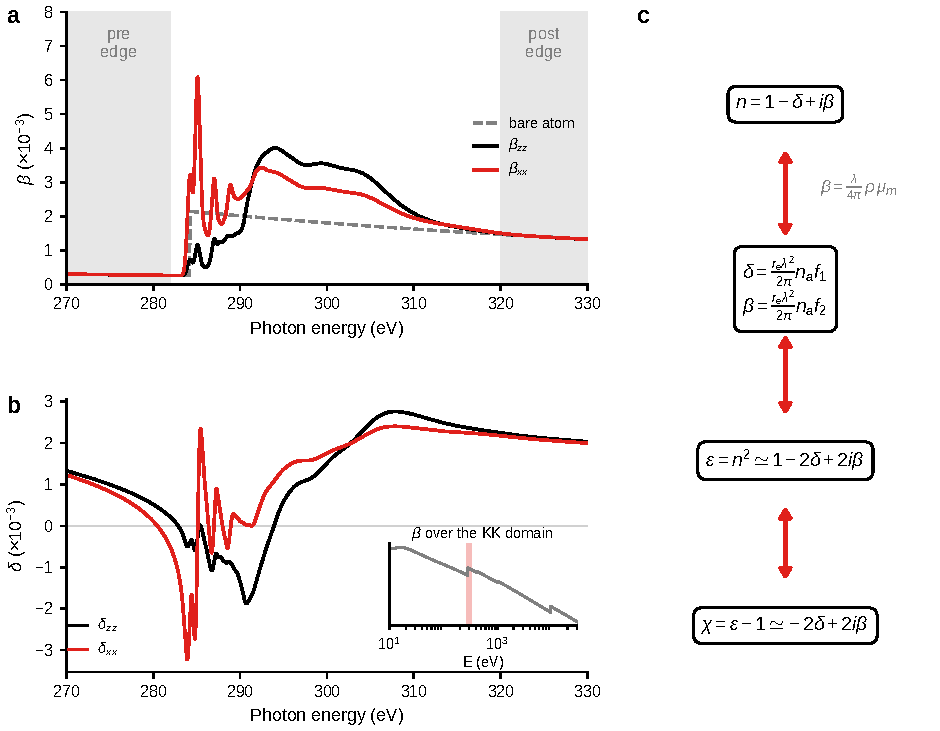
\includegraphics[width=\linewidth,height=0.75\textheight,keepaspectratio]{fig2-03_optical-constants}
  \caption[Optical constants of the \cref{chap:znpc} ZnPc film.]{Optical constants of the \cref{chap:znpc} ZnPc film. (a) In-plane \(\beta_{xx}\) (red) and out-of-plane \(\beta_{zz}\) (black) from the refined building-block model, with the bare-atom absorption (gray, dashed) and the pre-edge (270 to \qty{282}{eV}) and post-edge (320 to \qty{330}{eV}) normalization windows shaded. (b) \(\delta_{xx}\) and \(\delta_{zz}\) from the Kramers-Kronig transform of β. The inset shows the bare-atom β from \qty{10}{eV} to \qty{30}{keV} that closes the transform, with the measured window in red. (c) Relations between the refractive index n, the atomic scattering factors f1 and f2, the permittivity ε, and the susceptibility χ, with β = λρμm/(4π) linking β to the mass absorption μm.}
  \label{fig:2.5}
\end{figure}

\Cref{fig:2.5} carries these relations through for the ZnPc film of \cref{chap:znpc}. The absorptive part follows from the mass absorption through \(\beta = \lambda\rho\mu_{m}/(4\pi)\),\autocite{attwood1999soft} with the measured spectrum scaled to the bare-atom absorption of ZnPc\autocite{henke1993x} in a pre-edge window (270 to \qty{282}{eV}) and a post-edge window (320 to \qty{330}{eV}), where molecular bonding no longer alters the cross section (\cref{fig:2.5}a). Between the windows the edge-on texture splits \(\beta\) into two tensor components. The \(\pi^{*}\) resonances near \qty{285}{eV} appear almost entirely in \(\beta_{xx}\), since their transition dipoles lie along the ring normal and therefore close to the film plane, while the \(\sigma^{*}\) band above \qty{290}{eV} is stronger in \(\beta_{zz}\). The dispersive part follows from the Kramers-Kronig relation above (\cref{fig:2.5}b), evaluated by exact integration of a piecewise-linear \(\beta\), a special case of the piecewise-polynomial method of Watts.\autocite{watts2014calculation} Because \(\delta\) at each energy depends on \(\beta\) at every energy, the measured window is embedded in the bare-atom \(\beta\) from \qty{10}{eV} to \qty{30}{keV} before the transform is evaluated (\cref{fig:2.5}b, inset). The transform turns each absorption peak into a dispersive feature, so \(\delta_{xx}\) reaches about \(- 3 \times 10^{- 3}\) just below the first \(\pi^{*}\) resonance and changes sign across it, and both components approach a positive, slowly varying value well above the edge. Contrast in a resonant measurement therefore changes in sign as well as magnitude with energy. The energy of greatest contrast between two components therefore need not coincide with an absorption peak. \Cref{fig:2.5}c collects the equivalent descriptions of the same response, the atomic scattering factors \(f_{1}\) and \(f_{2}\), the permittivity \(\epsilon = n^{2}\), and the susceptibility \(\chi = \epsilon - 1\), so that results stated in any of these conventions can be compared directly.\autocite{attwood1999soft,yan2013accurate}

A fit that treats δ and β as independent at every energy can return optical constants that no causal material could have, with the dispersion at one energy unrelated to the absorption across the edge. Tying every resonance to a Gaussian and Dawson pair removes that freedom, since the dispersion at any energythen follows from the same few parameters that describe the absorption. Those parameters are the energy, width, strength, and dipole of each transition, and the next section takes them from DFT.

\section{Transitions from ML-Refined DFT}\label{sec:transitions-from-ml-refined-dft}

\begin{figure}
  \centering
  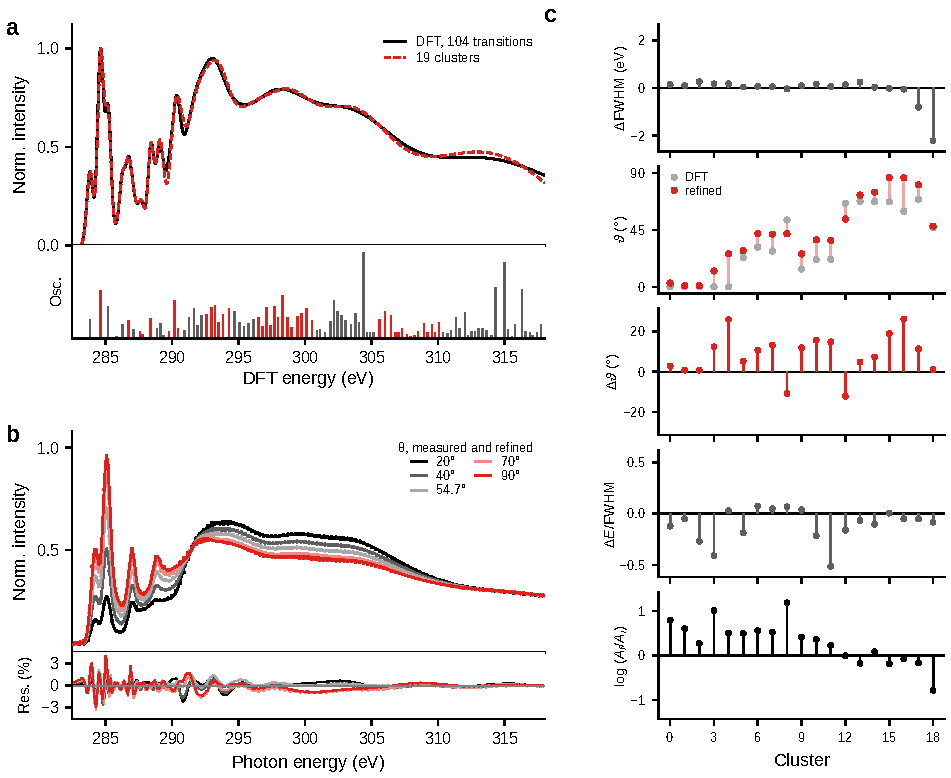
\includegraphics[width=\linewidth,height=0.75\textheight,keepaspectratio]{molecular-chapter/molch_dft}
  \caption[From DFT transitions to a refined cluster model of ZnPc.]{From DFT transitions to a refined cluster model of ZnPc. (a) Spectrum broadened from the 104 DFT transitions (black) against the sum of the 19 cluster Gaussians (red, dashed), on the DFT energy scale and normalized to its maximum. Below, each transition as a stick of height proportional to its oscillator strength, alternating in color between adjacent clusters. (b) Angle-resolved NEXAFS at θ = \ang{20} to \ang{90} (points) with the refined cluster model (lines), and the residuals as a percentage of the largest measured intensity. (c) Change of each cluster parameter from the DFT seed to the refined model, by cluster index in order of energy. From top, the change in full width at half maximum, the transition dipole angle ϑ from the ring normal for the seed (gray) and the refined model (red), its change Δϑ, the energy shift normalized by the seed width, and the logarithm of the ratio of refined to seed amplitude, each set of amplitudes normalized to its total. Seed energies include the rigid shift of \qty{0.45}{eV}.}
  \label{fig:2.6}
\end{figure}

The oscillators of a molecule can be taken from a measured spectrum or computed from its electronic structure. A measured spectrum fixes the total absorption at each energy but cannot say which transitions produce it, along which directions their dipoles point, or how much of the measured dichroism belongs to the molecule rather than to its orientation in the film. A calculation supplies all three, but its absolute energies carry an offset, its line widths are imposed by a chosen broadening rather than computed, and it treats an isolated molecule without the intermolecular interactions or vibronic structure of a film, so its spectrum departs from a measured one in energy, width, and relative strength. The approach used here, developed by Murcia,\autocite{murcia2026quantitative} combines the two (\cref{fig:2.6}). DFT supplies the transitions, clustering reduces them to the few that a spectrum can resolve, and refinement against angle-resolved NEXAFS adjusts the clusters while keeping the information the calculation carried.

The transitions of ZnPc were computed for a single molecule with the StoBe code by the transition-potential method with a half core hole, which yields the energy, oscillator strength, and transition dipole of every excitation, while \(\Delta KS\) calculations of the ground and core-excited states fix the absolute energy of each excitation center.\autocite{murcia2026quantitative} One calculation is made for each of the four inequivalent carbon sites, with the molecular geometry taken from the crystal structure, which agreed with experiment better than geometries relaxed thermodynamically or with force fields (Supplemental Material). Each transition carries the site from which it starts and the molecular orbital into which it excites, so every feature of the computed spectrum can be traced to a bond. The calculation treats an isolated molecule and so contains no states shared between neighbors, and its absolute energy scale carries an error of a few tenths of an electron volt, corrected by a rigid shift of \qty{0.45}{eV} before comparison with experiment.

A calculation of this kind returns more transitions than any spectrum resolves. The filtered calculation for ZnPc contains 104 transitions between 283.8 and \qty{318.4}{eV}, many of them separated by less than their own width and sharing a dipole direction (\cref{fig:2.6}a). Hierarchical agglomerative clustering groups such transitions into clusters, each standing for a family that no measurement could separate and carrying its own energy, width, strength, and dipole. Two hyperparameters control the grouping, a threshold on oscillator strength (OS) and a threshold on the overlap between neighboring line shapes (OVP). Both were scanned and each clustering compared with measured NEXAFS and with the original calculation, which selected OS = 0.25 and OVP = 52.5, with similar results for any OVP between 50 and 55 (Supplemental Material). The resulting 19 clusters reproduce the broadened calculation across the edge, with small departures near \qty{290}{eV} and at the highest energies.

Refinement then fits the clusters to angle-resolved NEXAFS of an edge-on film measured at five angles (\cref{fig:2.6}b). The energy, width, strength, and dipole direction of each cluster are adjusted together with the tilt that projects the molecular tensor into the frame of the film. The refined model reproduces the spectra at every angle with an average deviation of 2.7 percent (\cref{chap:znpc}), and its largest residuals fall on the narrow π* features. The changes the refinement makes are recorded cluster by cluster in \cref{fig:2.6}c. Widths broaden by up to about a quarter of an electron volt except in the two highest clusters, which narrow. Energies move by less than a width. The dipoles of the lowest π* clusters stay along the ring normal, the σ* clusters rotate further into the ring plane, and strength moves from the broad clusters above the edge toward the resolved resonances below it. Because each change is modest, every refined cluster remains identifiable with its seed and keeps the site and orbital assignment inherited from DFT.

The construction has two limits, both anticipated in the first question of \cref{chap:introduction}. The refinement is made against a reference film whose own orientation enters its dichroism, so the dipole of each cluster and the tilt of the film are fixed by the same data and are correlated. Clustering also keeps only the transitions selected as principal, so a weak transition, or one that appears only in a different molecular environment, has no cluster to represent it. \Cref{chap:znpc} tests the first limit by comparing the tilt recovered from reflectivity with the tilt of the reference, and \cref{chap:resonances} tests the second by refining the strength of individual clusters with depth.

\section{Molecular and Film Reference Frames}\label{sec:molecular-and-film-reference-frames}

The refined clusters describe one molecule. Each cluster is a Gaussian and Dawson pair attached to a unit dipole, and together with the bare-atom absorption that carries the edge step they fix the response of the molecule at every energy and polarization. A film contains many molecules in many orientations, and its response follows from how the frame of the molecule is distributed relative to the substrate.

The anisotropy of a molecular film originates in the orientation of its transition dipole moments. Each resonance couples most strongly to light polarized along its transition dipole and not at all to light polarized perpendicular to it, so the molecular optical tensor is a sum over transitions of the outer product \(\widehat{\mu}{\widehat{\mu}}^{T}\) of each unit transition dipole, weighted by the oscillator strength and line shape of that transition. For a planar conjugated molecule the C 1s → π* dipoles lie along the ring normal while the σ* dipoles lie largely in the ring plane, so the π* resonances enter the out-of-plane component of the molecular tensor and the σ* resonances its in-plane components (\cref{fig:2.3}c). The film tensor then follows from how the molecular frame is distributed relative to the substrate, and takes one of the three forms below.

\begin{equation}
  n_{\mathrm{iso}} = \begin{pmatrix} xx & 0 & 0 \\ 0 & xx & 0 \\ 0 & 0 & xx \end{pmatrix},\quad
  n_{\mathrm{uni}} = \begin{pmatrix} xx & 0 & 0 \\ 0 & xx & 0 \\ 0 & 0 & zz \end{pmatrix},\quad
  n_{\mathrm{bi}} = \begin{pmatrix} xx & 0 & 0 \\ 0 & yy & 0 \\ 0 & 0 & zz \end{pmatrix}.
  \label{eq:tensor-symmetry}
\end{equation}

The most general film response is a fully biaxial tensor, but most molecular films instead adopt one of the two simpler limits shown above. An isotropic film, with all three axes equal, requires the molecular ensemble to be fully randomized in three dimensions. More commonly due to processing methods, physical vapor deposition and solvent process techniques like spin coating order a single molecular axis, such as the macrocycle normal, relative to the substrate normal while leaving the in-plane azimuthal distribution unconstrained, producing the uniaxial case considered throughout this work.

\begin{figure}[htp]
  \centering
  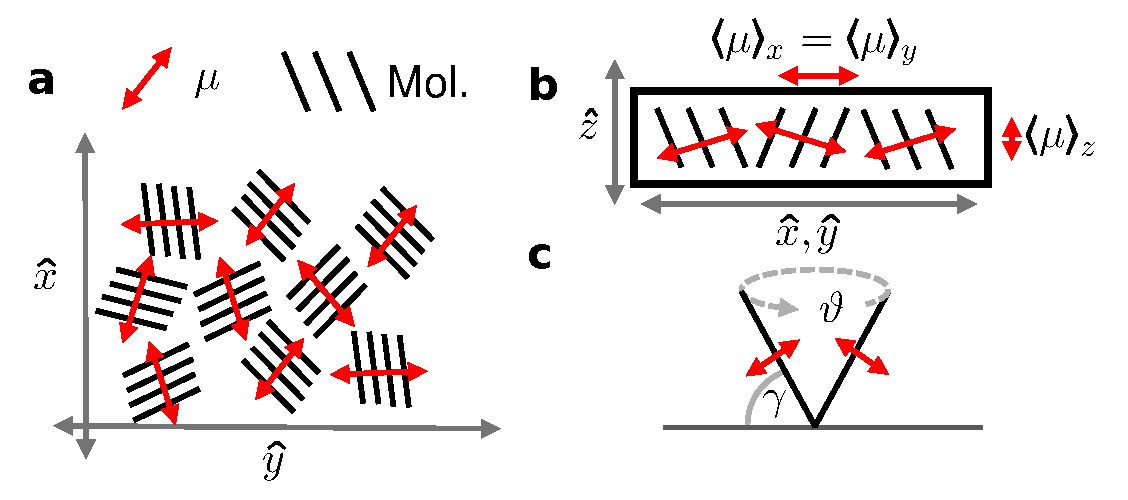
\includegraphics[width=0.75\linewidth,height=0.75\textheight,keepaspectratio]{fig2-07_tensor-construction}
  \caption[Schematic construction of a uniaxial molecular film.]{Schematic construction of a uniaxial molecular film. Molecular crystallites are drawn with their transition dipole moments μ. (a) In-plane distribution of crystallites, evenly distributed in azimuth across the film. (b) Film cross section with distinct in-plane and out-of-plane averaged dipoles. (c) Ensemble average over the tilt γ between the molecular plane and the substrate, equal to the tilt of the ring normal from the surface normal, and over in-plane rotations ϑ.}
  \label{fig:2.7}
\end{figure}

Explicitly, a uniaxial molecular tensor \(n^{m} = \operatorname{diag}\left( n_{xx}^{m},n_{xx}^{m},n_{zz}^{m} \right)\) tilted by \(\gamma\) about the in-plane \(x\) axis and averaged over the azimuthal rotation \(\vartheta\) sketched in \cref{fig:2.7} gives the film tensor

\begin{equation}
  n^{f}(E;\gamma,\rho) = \frac{\rho}{2\pi}\int_{0}^{2\pi} R_{z}(\vartheta)\, R_{x}(\gamma)\, n^{m}(E)\, R_{x}(\gamma)^{\mathsf{T}}\, R_{z}(\vartheta)^{\mathsf{T}}\, d\vartheta,
  \label{eq:film-tensor}
\end{equation}

whose diagonal components are

\begin{align}
  n_{xx}^{f}(E;\gamma,\rho) &= \frac{\rho}{2}\left[ n_{xx}^{m}\left( 1 + \cos^{2}\gamma \right) + n_{zz}^{m}\sin^{2}\gamma \right], \label{eq:film-xx}\\
  n_{zz}^{f}(E;\gamma,\rho) &= \rho\left( n_{xx}^{m}\sin^{2}\gamma + n_{zz}^{m}\cos^{2}\gamma \right), \label{eq:film-zz}
\end{align}

recovering the molecular values at \(\gamma\  = \ 0\) as expected for a rotation of a uniaxial tensor. \(n_{xx}\) carries an additional factor of \((1 + cos²\gamma)/2\) rather than simply \(cos²\gamma\) because it is further averaged over the in-plane azimuthal angle \(\vartheta\), whereas \(n_{zz}\), fixed along the rotation axis, requires no such averaging. The trace is conserved, \(2n_{xx}^{f} + n_{zz}^{f} = \rho\left( 2n_{xx}^{m} + n_{zz}^{m} \right)\) for every \(\gamma\), which provides a direct check of any implementation. Supplemental Material extends this relation to a partially ordered ensemble of finite density \emph{ρ}, the form used throughout the structural fits in \cref{chap:znpc,chap:resonances}.

\section{Angle-Resolved NEXAFS of a Uniform Film}\label{sec:angle-resolved-nexafs-of-a-uniform-film}

\begin{figure}[htp]
  \centering
  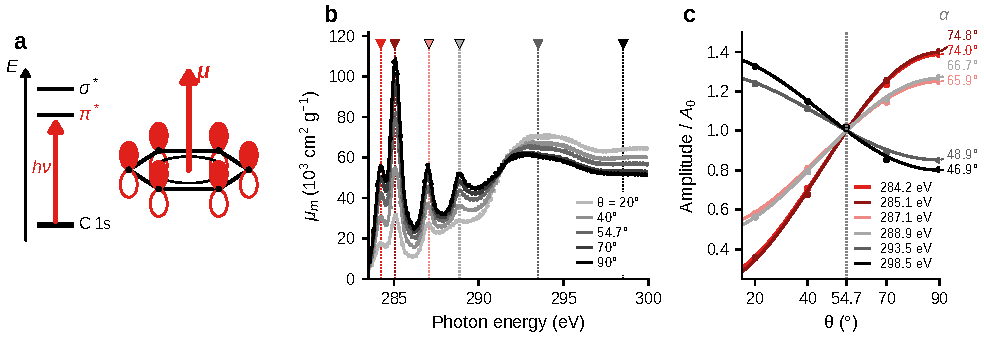
\includegraphics[width=\linewidth,height=0.75\textheight,keepaspectratio]{fig1-02_ar-nexafs}
  \caption[Angle-resolved NEXAFS of an edge-on ZnPc film, resolved by transition cluster.]{Angle-resolved NEXAFS of an edge-on ZnPc film, resolved by transition cluster. (a) Energy diagram for a C 1s → π* excitation, and a conjugated carbon ring above the substrate with the p orbitals that form its π* states normal to the ring plane. The transition dipole μ of a C 1s → π* excitation points along the ring normal, at angle α from the surface normal n. (b) Mass absorption \(\mu_{m}\) from 283.5 to \qty{300}{eV} with the electric field at θ = \ang{20} to \ang{90} from the surface normal (light to dark gray points), with fits built from the cDFT clusters (lines). Triangles mark the six clusters shown in c. (c) Amplitude against θ for six representative clusters, normalized by the isotropic amplitude \(A_{0}\), with fits to the vector-orbital form \(A_{0}[1 + (1/2)(3\cos^{2}\theta - 1)(3\cos^{2}\alpha - 1)]\). The fitted transition dipole angle α is printed at the right of each curve.}
  \label{fig:2.8}
\end{figure}

Angle-resolved NEXAFS of the edge-on ZnPc film tests the simplest film this construction allows, one in which every molecule shares a single tilt (\cref{fig:2.8})\autocite{stohr2010nexafs,ade2008nexafs}. The \(\pi^{*}\) states are built from p orbitals that stand above and below the conjugated ring, so the transition dipole \(\mathbf{\mu}\) of a C 1s \(\rightarrow \pi^{*}\) excitation points along the ring normal, at an angle \(\alpha\) from the surface normal \(\widehat{\mathbf{n}}\) of a film. By Fermi's golden rule the absorption scales as \(\left| \mathbf{E} \cdot \mathbf{\mu} \right|^{2}\), so rotating \(\mathbf{E}\) from \(\theta\) = \ang{20} to \ang{90} relative to \(\widehat{\mathbf{n}}\) in an edge-on ZnPc film raises the \(\pi^{*}\) resonances near \qty{285}{eV} and lowers the \(\sigma^{*}\) band above \qty{291}{eV} (\cref{fig:2.8}b). Integrating fixed energy windows would mix overlapping transitions under one assumed orbital symmetry. Instead, each spectrum is decomposed into the 16 cDFT transition clusters between 283.5 and \qty{300}{eV}, with centers and widths fixed and one non-negative amplitude per cluster and angle, which reproduces every spectrum with a relative residual below 3 percent. The amplitude of each cluster follows the vector-orbital form \(A_{0}\,[1 + (1/2)(3\cos^{2}\theta - 1)(3\cos^{2}\alpha - 1)]\) (\cref{fig:2.8}c), which gives each cluster its own dipole angle \(\alpha\). The three lowest \(\pi^{*}\) clusters give \(\alpha\) = 74.0 to \ang{74.8}. Clusters between 286 and \qty{291}{eV} fall progressively from \ang{72} to \ang{60}, while the \(\sigma^{*}\) clusters above \qty{293}{eV} give 47 to \ang{49}, below the magic angle of \ang{54.7} at which a uniaxial film shows no dichroism. In a uniaxial film these angles map onto one ring tilt \(\gamma\) through the direction of each dipole in the molecular frame, with \(\alpha = \gamma\) for a dipole along the ring normal and \(\cos^{2}\alpha = (1/2)\sin^{2}\gamma\) for one in the ring plane. A single tilt of \ang{68.2} reproduces the \(\sigma^{*}\) clusters but leaves the \(\pi^{*}\) clusters \ang{6} steeper, a discrepancy that no uniform tilt removes. Angle-resolved NEXAFS therefore measures orientation cluster by cluster, but recovering the molecular state from it requires the tensor treatment developed in this chapter and in \cref{chap:methods,chap:znpc}, which places the bulk tilt at \(\gamma\) = \ang{69.6} within a depth gradient.

Four values of the ZnPc tilt appear in this dissertation, and each answers a different question. The value of \ang{62} is the starting point of the refinement and carries no information about the film. The final step of the refinement fits one tilt to the full set of spectra with the dipoles at their calculated directions and returns \ang{74}, the value reported in \cref{chap:znpc} and Supplemental Material. That fit is dominated by the strong π* resonances, whose dipoles lie along the ring normal and report the tilt directly, and it agrees with the 74.0 to \ang{74.8} found above for the three lowest π* clusters. The single tilt that best reproduces the cluster angles is \ang{68.2}, set mainly by the σ* clusters. Polarized reflectivity resolves the film in depth and places the bulk at \ang{69.6(2)}, with \ang{58.7(6)} at the free surface and \ang{38(1)} at the oxide (\cref{tab:4.1}). A depth gradient of this kind, weighted differently by each measurement, is consistent with the spread between \ang{68} and \ang{74}, although a small error in the calculated σ* dipole directions could contribute as well.

A film built in this way has a fixed number of optical parameters. The refined clusters fix the response of the molecule at every energy and polarization, so each layer of a film is specified by its tilt and density however many energies are measured. This property underlies both questions of the dissertation. It makes the structural fits of \cref{chap:znpc} tractable with an order of magnitude fewer parameters than a free tensor, and it leaves room in \cref{chap:resonances} to refine the strength and orientation of individual resonances with depth without the fit becoming underdetermined.

The failure of a uniform tilt to describe ZnPc motivates resolving the film in depth, which the reflectivity methods of \cref{chap:methods} provide. The construction also rests on a reference spectrum measured once and then reused, which raises the third open problem of this work, whether a spectrum measured on one film can be trusted when it is applied to another. \Cref{chap:xray-atlas} addresses that problem through a shared, versioned record of spectra and of the optical models built from them.

\chapter{Fundamentals and Methods of Polarized Resonant Soft X-ray Reflectivity}\label{chap:methods}

This chapter develops the physical and practical framework used in every later chapter. It first describes what a far-field scattering measurement records and why specular reflectivity, unlike transmission scattering, must be computed beyond the Born approximation. It then introduces the gradient model used for interfacial structure in Chapter 4, built on the film tensor of Chapter 2. The remaining sections describe how polarized resonant reflectivity is measured at ALS beamline 11.0.1.2, from alignment through reduction, stitching, and uncertainty, and how it is analyzed, from the forward model through optimization, posterior estimation, and model selection.

\section{\texorpdfstring{Scattering in the Far Field}{Scattering in the Far Field}}\label{figmarker9x-scattering-in-the-far-field}

\begin{figure}[tbp]
  \centering
  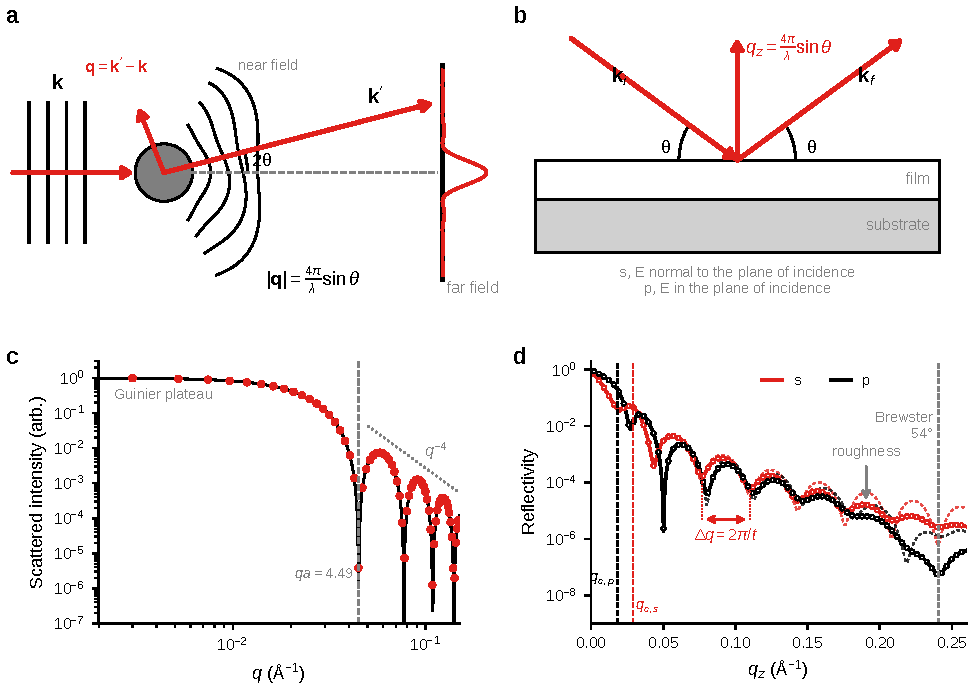
\includegraphics[width=\linewidth,height=0.75\textheight,keepaspectratio]{fig2-01_scattering-geometry}
  \caption[Scattering geometries and the momentum transfer.]{Scattering geometries and the momentum transfer. a) A plane wave with wavevector k scatters from a finite object, and the curved near-field wavefronts flatten into the far-field pattern recorded along k\ensuremath{'} at scattering angle 2θ. The momentum transfer is q = k\ensuremath{'} − k, with |q| = (4π/λ) sin θ. b) Specular reflection from a film on a substrate at grazing angle θ, for which qz = (4π/λ) sin θ lies along the film normal. s polarization places E normal to the plane of incidence and p polarization places E in it.}
  \label{fig:3.1}
\end{figure}


Every measurement in this work records intensity in the far field as a function of the momentum transfer \(\mathbf{q} = \mathbf{k}' - \mathbf{k}\) between the incident and scattered wavevectors (Fig.~\ref{fig:3.1}). For elastic scattering \(\left| \mathbf{k} \right| = \left| \mathbf{k}' \right| = 2\pi/\lambda\), so the magnitude \(\left| \mathbf{q} \right| = (4\pi/\lambda)\sin\theta\) is fixed by the scattering angle \(2\theta\) alone (Fig.~\ref{fig:3.1}a).\autocite{attwood1999soft} In transmission RSoXS, \(\mathbf{q}\) is read from the position of the diffuse intensity on an area detector, with the pattern reporting in-plane structure through its dependence on \(\left| \mathbf{q} \right|\).\autocite{collins2012polarized,gann2016origins,grabner2025resonant} Specular reflectivity instead holds the detector at twice the grazing angle, so the reflected beam leaves at the angle of incidence and \(\mathbf{q} = q_{z}\widehat{\mathbf{z}}\) lies along the film normal (Fig.~\ref{fig:3.1}b). To first order, scanning \(\theta\) then samples the Fourier components of the depth profile of the optical constants, which is why reflectivity resolves stratification that transmission averages over.\autocite{wang2005soft,wang2007resonant} The plane of incidence also defines the two polarizations used throughout. In s polarization \(\mathbf{E}\) lies normal to the plane of incidence and therefore in the film plane at every \(\theta\). In p polarization \(\mathbf{E}\) lies in the plane of incidence and carries a component \(\cos\theta\) along the film normal, largest at grazing incidence. For a uniaxial film the two polarizations therefore weight the in-plane and out-of-plane components of the optical tensor differently, which is the source of the orientation sensitivity used in Chapters 4 and 5.\autocite{mezger2011molecular,thelen2020molecular}

The far-field condition is stated through the Fresnel number \(F = a^{2}/(L\lambda)\), which compares the size \(a\) of a scattering feature with the distance \(L\) to the detector and the wavelength \(\lambda\).\autocite{foldy1945multiple} At 284 eV, \(\lambda \approx 4.37\) nm, and for \(a = 10\) nm domains with \(L \approx 0.5\) m, \(F \approx 5 \times 10^{- 8}\). \(F\) approaches unity only for structures near \((L\lambda)^{1/2} \approx 47\) µm, far larger than any feature studied here, so every measurement in this work is a Fraunhofer measurement. This condition concerns the detector and says nothing about the field inside the sample. Figure~\ref{fig:3.2} follows a plane wave through a small cluster of scatterers with a two-dimensional multiple-scattering calculation. Near the cluster each scatterer is driven by the incident wave and by the fields scattered from its neighbors, so the crests of the total field are distorted\autocite{lax1951multiple,foldy1945multiple}, with a scatterer deep in the cluster radiating in response to both. With distance these distortions propagate out into smooth outgoing wavefronts, and the detector records only the far-field intensity \(I(2\theta)\), a forward peak set by the spacing and size of the scatterers with weaker side maxima. The measurement therefore discards the phase of the far field and the structure of the near field, and the sample must be inferred by forward modeling and fitting, as described in the section on fitting. When the interaction between scatterers is weak, one scattering event per photon suffices and the first Born approximation \(A\left( \mathbf{q} \right) = \int\Delta n\left( \mathbf{r} \right)\, e^{i\mathbf{q} \cdot \mathbf{r}}\, d^{3}r\) applies, which is the basis of transmission RSoXS and of its simulation.\autocite{collins2022resonant,gann2016origins,saurabh2023textless,dudenas2025how,grabner2024molecular} When it is strong, as for specular reflection near the critical angle, the multiple scattering of Fig.~\ref{fig:3.2} must be solved exactly, which the transfer matrix method of Fig.~\ref{fig:3.6} does for a layered film.

\begin{figure}[tbp]
  \centering
  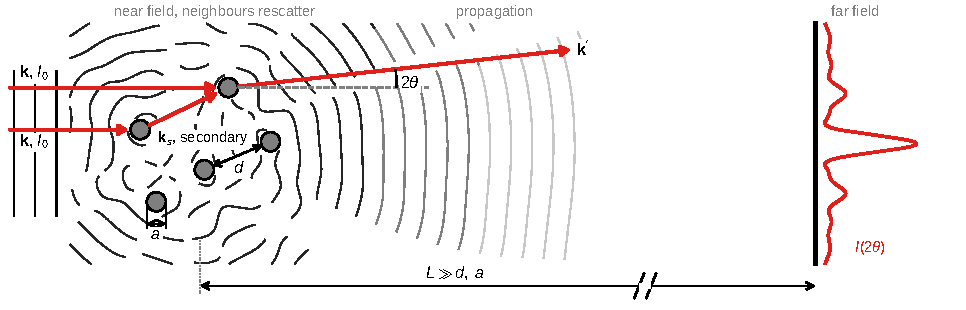
\includegraphics[width=\linewidth,height=0.75\textheight,keepaspectratio]{fig2-02_near-far-field}
  \caption[The far-field pattern emerges from local interactions between scatterers.]{The far-field pattern emerges from local interactions between scatterers. A plane wave with wavevector k and intensity I0 illuminates five scatterers of size a separated by distances of order d. The front scatterer scatters forward along ks, so a deeper scatterer is driven by both I0 and this secondary field before it radiates along k\ensuremath{'}. Black lines are crests of the total scattered field from a two-dimensional multiple-scattering (Foldy-Lax) calculation, distorted near the cluster and flattening into outgoing wavefronts with distance. A detector at L ≫ d, a records only the far-field intensity I(2θ) (red), and the L axis is broken.}
  \label{fig:3.2}
\end{figure}


\section{Why Specular Reflectivity Is Not Kinematic}\label{why-specular-reflectivity-is-not-kinematic}

Specular reflectivity is the measurement in this work for which the first Born approximation fails. Below the critical angle \(\theta_{c} = (2\delta)^{1/2}\) reflection is nearly total, and near \(\theta_{c}\) the reflected amplitude is comparable to the incident amplitude, so the field inside the film differs from the incident field and waves reflected between interfaces interfere with one another.\autocite{parratt1954surface} Far above \(\theta_{c}\) the kinematic result \(R\left( q_{z} \right) \approx R_{F}\left( q_{z} \right)\left| \delta_{\infty}^{- 1}\int(d\delta/dz)\, e^{iq_{z}z}\, dz \right|^{2}\) holds, where \(R_{F}\) is the Fresnel reflectivity of the bare substrate, \(\delta(z)\) the depth profile of the refractive decrement, and \(\delta_{\infty}\) its value in the substrate.\autocite{alsnielsen2011elements} It is used here only to read two features of the data. \(R_{F}\) decays as \(q_{z}^{- 4}\), which the \(Rq_{z}^{4}\) representation used in later chapters removes, and a layer of thickness \(t\) produces Kiessig fringes spaced by \(\Delta q_{z} \approx 2\pi/t\), so the fringe period reports the thickness directly.\autocite{kiessig1931interferenz} Near \(\theta_{c}\), where the data are most intense, the reflectivity is instead computed exactly in one dimension by the transfer matrix method described in the section on simulating reflectivity, so no perturbative approximation enters the fits in this work.

\section{Orientation gradient theoretical foundation}\label{orientation-gradient-theoretical-foundation}

We formulate our gradient model from a Ginzburg-Landau framework of second order phase transitions, where we treat the molecular orientation and density as order parameters (not to be confused with nematic order parameters \(S(\gamma)\) or \(P(\gamma)\)).\autocite{gennes2023physics,ginzburg2009theory} Along the one dimensional depth axis \(z\) of a film of thickness \(L\), we take the order parameters as the deviation in the density \(\Delta\rho(z) = \rho(z) - \rho_{b}\) and orientation \(\Delta\gamma(z) = \gamma(z) - \gamma_{b}(z)\) from the bulk. The total free energy of the film is described by the functional

\[\begin{array}{r}
F\lbrack\Delta\rho,\Delta\gamma\rbrack = \int_{0}^{L}{f(\Delta\rho,\Delta\gamma) + \frac{1}{2}c_{\rho}\left( {\Delta\rho}' \right)^{2} + \frac{1}{2}c_{\gamma}\left( {\Delta\gamma}' \right)^{2}dz} \\
 + F_{v}\left\lbrack \Delta\rho(0),\Delta\gamma(0) \right\rbrack + F_{Si}\left\lbrack \Delta\rho(L),\Delta\gamma(L) \right\rbrack
\end{array}\]

Here \(f(\Delta\rho,\Delta\gamma)\) is the local bulk free energy density, and the terms proportional to \(c_{\rho}\) and \(c_{\gamma}\) are the gradient energy penalties that oppose abrupt variations within the film. The interface terms \(F_{v}\) and \(F_{Si}\) account for the anchoring potentials at the interface boundaries. Expanding \(f(\Delta\rho,\Delta\gamma)\) to quadratic order about the bulk minimum,

\[\begin{array}{r}
f(\Delta\rho,\Delta\gamma) \approx f_{0} + \frac{1}{2}a_{\gamma}{\Delta\gamma}^{2} + \frac{1}{2}a_{\rho}{\Delta\rho}^{2} + b\Delta\rho\Delta\gamma.
\end{array}\]

where \(a_{\rho}\) and \(a_{\gamma}\) are the stability coefficients of the bulk phase, and \(b\) the bilinear coupling term between the density and orientation fields.

Minimizing the total variation \(\delta F = 0\) and integrating the gradient terms by parts yields a system of coupled second-order differential equations for the film interior,

\[{\begin{array}{r}
c_{\rho}{\Delta\rho}^{''} = a_{\rho}\Delta\rho + b\Delta\gamma\ 
\end{array}
}\begin{array}{r}
c_{\gamma}{\Delta\gamma}^{''} = a_{\gamma}\Delta\gamma + b\Delta\rho\ 
\end{array}\]

with boundaries dictated by the surface free energies. To leading order in the interface fields \(h\), the boundary variation yields Robin boundary conditions, where the gradient of the order parameter is proportional to the surface field, i.e.

\[\begin{array}{rlr}
c_{\rho}\Delta\rho'(0) = - h_{\rho}^{v}\  & & c_{\rho}\Delta\rho'(L) = h_{\rho}^{Si}
\end{array}\]

and with similar form for \(\Delta\gamma\). When the surface fields \(h\) are much stronger than the bulk stiffness coefficients \(c/\tau\), the system enters the Dirichlet regime of strong anchoring, in which the interface potentials set the order parameters to fixed interfacial values, \(\Delta\rho(0) = {\Delta\rho}_{v}\) and \(\Delta\rho(L) = {\Delta\rho}_{Si}\). Within this regime the interfaces impose an orientational state regardless of the bulk interaction, a feasible state given the known different growth modes for ZnPc films at the substrate and surface.\autocite{derrien2022interfacial,yang2015molecular}

This system of equations may be decoupled into a normal modes problem, under the coordinate transform \(\widetilde{\Delta\rho} = \sqrt{c_{\rho}}\Delta\rho\) and similar transform for \(\Delta\gamma\). Given that the bulk represents the stable minimum, the general solution is restricted to the linear combination of exponentials decaying from the boundaries with coherence lengths \(\tau_{\pm}\) derived from the eigenvalues of the coupled system. When the orientation and density coupling is nonzero, these coherence lengths are shared between the order parameters. As each interface bears its unique interactions that dictate this coherence length, we assume that each interface is dominated by a single mode. The interface gradient model used in the main text satisfies these conditions,

\[{\begin{array}{r}
\Delta\rho(z) = \Delta\rho_{v}\exp\left( - z/\tau_{vac} \right) + \Delta\rho_{Si}\exp\left( - (L - z)/\tau_{Si} \right)
\end{array}
}\begin{array}{r}
\Delta\gamma(z) = \Delta\gamma_{v}\exp\left( - z/\tau_{vac} \right) + \Delta\gamma_{Si}\exp\left( - (L - z)/\tau_{Si} \right)\ 
\end{array}\]

While this model is congruent with the continuous reorientation under an evolving growth front, it remains an empirical approximation of the underlying interfacial physics. A more rigorous determination of the anchoring potentials would require a detailed investigation of the boundary conditions, specifically whether the system is governed by Dirichlet or Robin boundaries as this determines the relationship between exponential amplitudes and the interfacial potentials. Furthermore, this model assumes a continuous structural relaxation; however, it is possible that the molecular realignment across the interface occurs under a different mechanism than described here requiring a different theoretical basis.

\section{Polarized Resonant Reflectivity}\label{polarized-resonant-reflectivity}

Polarized resonant reflectivity measures the film tensor of the preceding sections as a function of depth. It is the only technique with demonstrated sensitivity to molecular orientation at buried heterointerfaces.\autocite{ferron2023composition,heilman2026sub} Orientation at such interfaces sets the performance of organic photovoltaic devices\autocite{tumbleston2014influence} and the efficiency of organic light-emitting diodes,\autocite{yokoyama2011molecular} yet few studies have resolved the depth profiles of orientation and composition together. The limitation lies in the analysis more than in the measurement, since existing frameworks were built for single systems and carry assumptions that fail elsewhere. The sections that follow describe the measurement and a general analysis framework for it. Every program and algorithm is open source and maintained jointly by the Collins group at WSU, the ALS computing group, and the beamline scientists at 11.0.1.2, where the analysis is being integrated into the beamline control system toward autonomous experimentation. The framework is demonstrated here for reflectivity but applies to RSoXS measurements generally.

\section{Experimental Methods}\label{experimental-methods}

Reflectivity complements the transmission geometries above by directly resolving depth, mapping a film\textquotesingle s optical constants as a function of distance from the surface rather than averaging over the full film thickness. Polarization further resolves the orientational anisotropy captured in the tensor framework above, since \emph{s} and \emph{p} polarized light couple to different components of the optical tensor at a given angle of incidence. Together, depth and polarization sensitivity make reflectivity the natural geometry for testing the orientation and chemical-state profiles this dissertation is built around.

X-ray reflectivity measures the specular reflected intensity, directly probing the reflection coefficients set by the refractive index of each layer. In multi-layered films, multiple reflections at each interface break the Born approximation requiring a rigorous simulation platform that can express these multiple reflection and transmission events. For anisotropic materials, the standard approach follows the transfer matrix method that recursively solves the reflection and transmission coefficients at the interfaces of thin slabs bearing uniform optical constants. This means that not only is the reflected intensity set by the surface optical constants, but also those buried in every layer below the surface, allowing the technique to resolve optical stratification that no other technique can. The final product of the technique is a depth profile of the optical constants along the depth of a film, and in polarized and resonant reflectivity, interpreting this profile is core to resolve molecular state as a function of depth.

Real interfaces are rough or graded, which damps the specular reflectivity at each interface and redistributes intensity into diffuse scattering. For organic films the distinction matters, since a sharp but rough interface and a gradual change of composition or orientation can damp the specular signal similarly while implying different physics at the interface. The interface models used in this work, and the regimes in which each applies, are described in the section on simulating reflectivity (Fig.~\ref{fig:3.7}).

\subsection{\texorpdfstring{Reflectivity setup at 11.0.1.2}{Reflectivity setup at 11.0.1.2}}\label{figmarker11x-reflectivity-setup-at-11.0.1.2}

\begin{figure}[tbp]
  \centering
  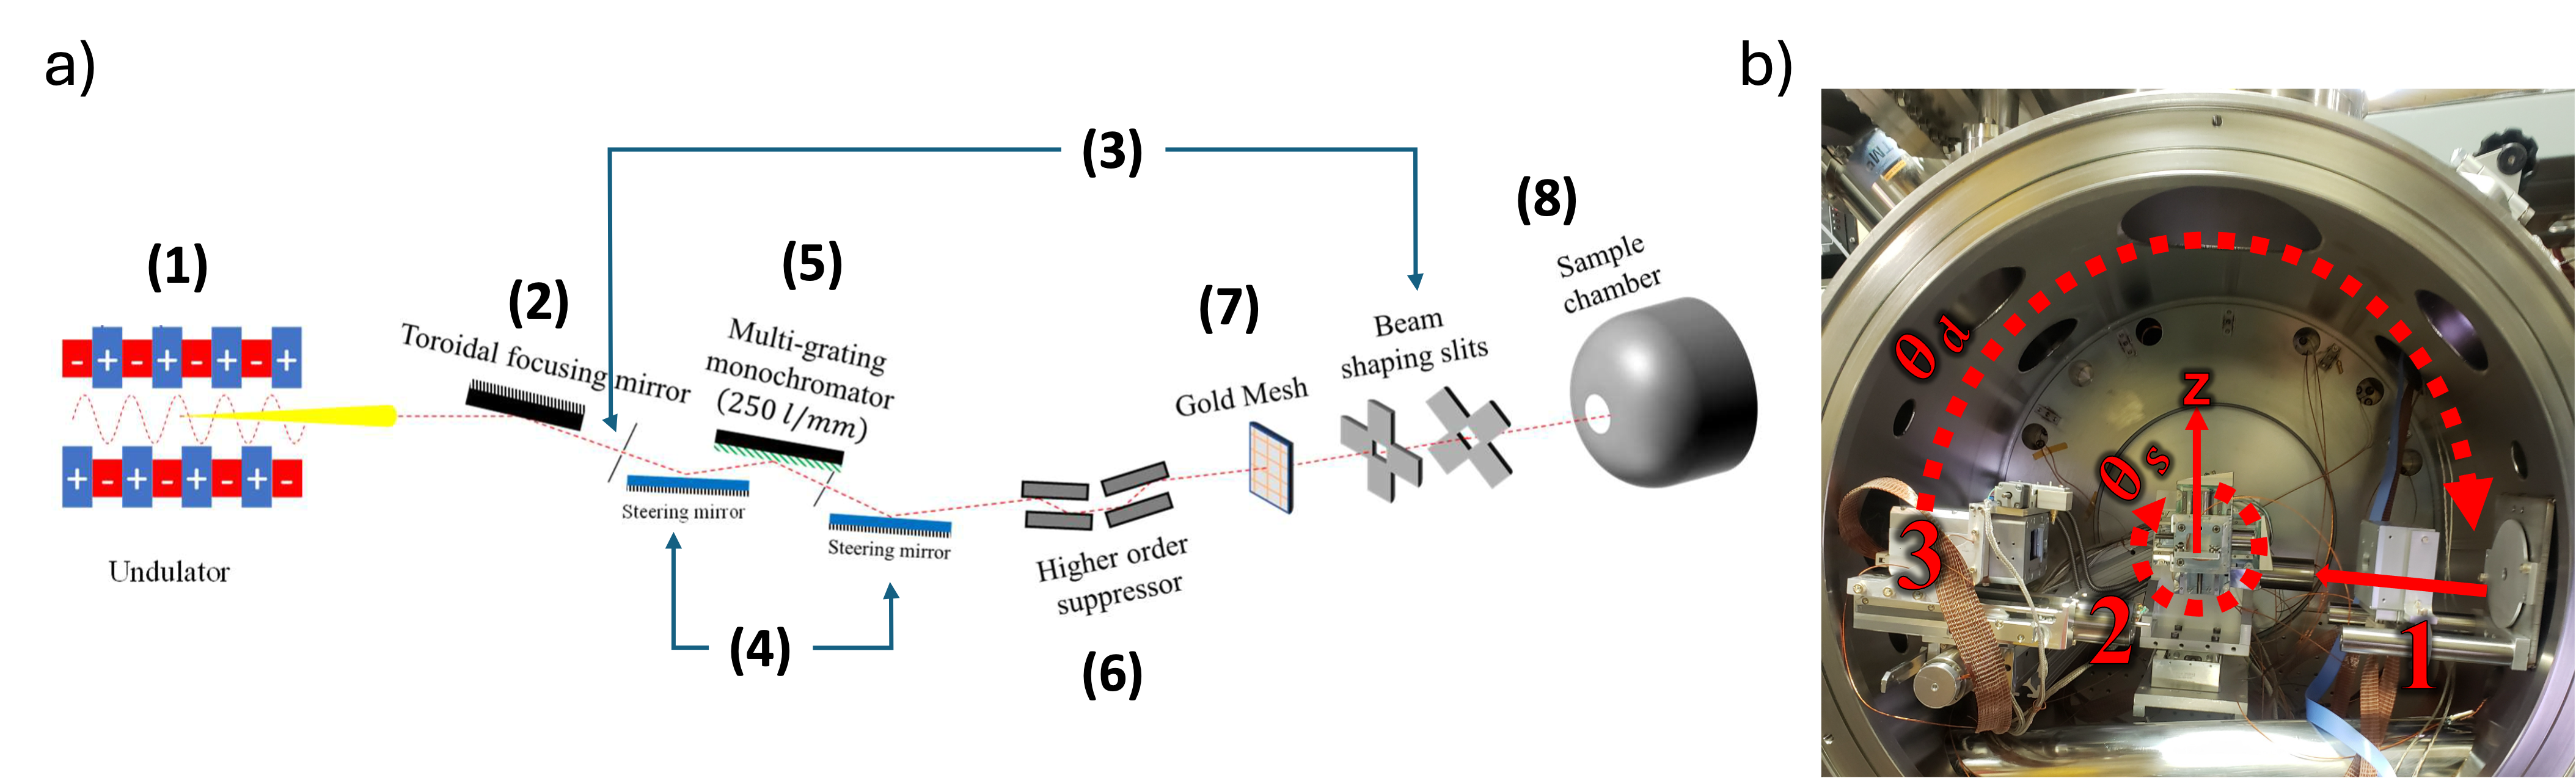
\includegraphics[width=\linewidth,height=0.75\textheight,keepaspectratio]{beamline-schematic}
  \caption[Beamline schematic of ALS Beamline 11.0.1.2.]{Beamline schematic of ALS Beamline 11.0.1.2. a) Optical path of X-rays: (1) UPS undulator injection source producing polarized photons, (2) toroidal focusing mirror, (3) beam shaping slits, (4) vertical deflection steering and focusing mirrors, (5) grating monochromator for energy selection, (6) higher order suppression optics to remove higher harmonics and linearly attenuate the beam, (7) gold mesh intensity monitor, (8) reflectometer chamber. b) Interior of the 11.0.1.2 chamber: (1) beam entrance path after leaving the beam shaping slits, (2) sample stage with four rotation axes, (3) area detector with three degrees of freedom mounted on a goniometer rotation arm with near coaxial rotation with the sample stage.}
  \label{fig:3.3}
\end{figure}


Resonant reflectivity is recorded on the area detector (Fig.~\ref{fig:3.3}b, 3) after reflection from the sample (Fig.~\ref{fig:3.3}b, 2), with each measurement following four steps.

\begin{enumerate}
\def\labelenumi{\arabic{enumi}.}
\item
  \textbf{Beam Shaping} -- The beam defining slits, higher order suppressor, and focusing mirrors are fine tuned to block anomalous scattering from the optical elements while lowering the intensity so the direct beam can safely be measured on the area detector without damage.
\item
  \textbf{Sample Alignment} -- The sample theta and height (Fig.~\ref{fig:3.3}b, \(\theta_{s}\) and \(z\) respectively) are iteratively aligned to the direct beam so that the \(\theta_{s} = 0\) corresponds to perfectly grazing, with \(z\) set to cut the beam intensity in half.
\item
  \textbf{Scan Definition} -- The experimental orchestration scan is configured to capture upwards of 10 orders of magnitude of signal as a function of sample and detector angles \(\theta_{s\ }\ \&\ \theta_{d}\) while maintaining normalizability.
\item
  \textbf{Scan Running and Monitoring} -- Finally, scans are monitored over the angular range watching for frames where the reflected intensity drops below the detector dynamic range, or for instances where the reflected intensity saturates the detector.
\end{enumerate}

This general procedure is repeated for each measurement condition (photon energy, photon polarization, etc.) to fully capture the samples reflectivity coefficients over these conditions. The exact procedures for this technique are evolving, with recent developments towards fully agentic data collection (Fig.~\ref{fig:3.12}).

\subsection{Sample Alignment}\label{sample-alignment}

Reflectivity normalization is performed by iteratively refining the sample height (sample \(z\) motor) and the sample \(\theta_{s}\) motors such that the beam is perfectly flat and cutting the beam in half. This is performed by exploiting the size of the beam itself. First using the nominal z and theta positions, the sample is rotated flat and below the beam. From there it is incrementally moved through the beam and the intensity is watched on the photodiode. This results in a sigmoid distribution that convolves the beam profile with edge of the sample and sample stage, a process known as a knife edge test. The place where the beam intensity is halved centers the topmost point of the sample into the center of the beam.

Next the \(\theta_{s}\) motor is scanned around zero degrees, \(\theta_{s} \in ( - 1{^\circ},1{^\circ})\). When the sample is poorly aligned, the photodiode bears a wide distribution centered around the point where the intensity is maximized. The sample \(\theta\) motor is then reset so that this angle is taken as \(0{^\circ}\) before returning to the

sample \(z\) alignment routine. As the alignment improves these distributions change shape, the sample z becomes a sharper distribution as it is no longer possible to reflect some of the incident beam as the sample moves into position. Yet the sample theta positions change more drastically.

\begin{figure}[tbp]
  \centering
  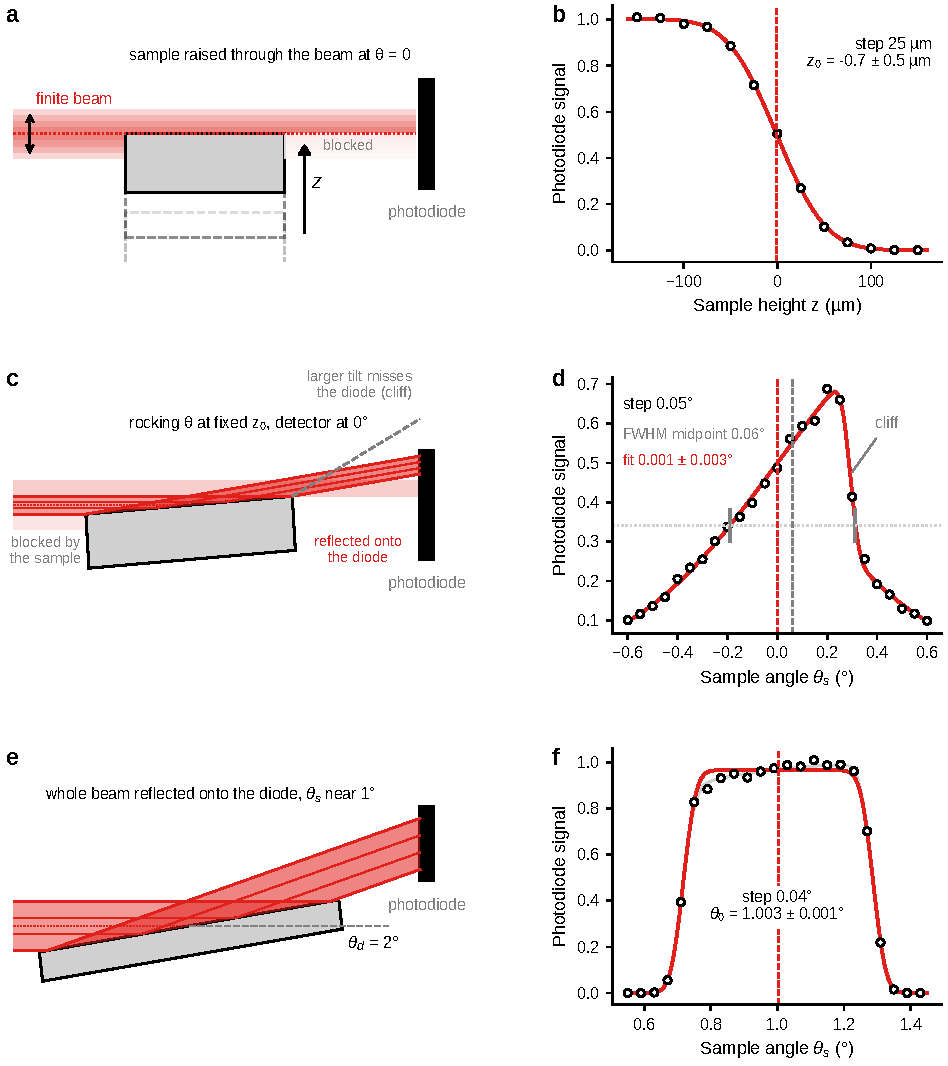
\includegraphics[width=\linewidth,height=0.75\textheight,keepaspectratio]{fig2-07_alignment}
  \caption[Sample alignment with a finite beam and a finite photodiode, simulated by ray Monte Carlo.]{Sample alignment with a finite beam and a finite photodiode, simulated by ray Monte Carlo. a, b) Knife-edge geometry, in which the sample is raised through the beam at θ = 0, and the photodiode signal in 25 µm steps with an error-function fit, which places the surface at z0 = −0.7 ± 0.5 µm for a beam of σ ≈ 41 µm. c, d) Rocking geometry at fixed z0 with the detector at 0°, where light reflected from the surface (dark red) adds to the unblocked beam until a larger tilt sends it over the diode (gray, dashed), and the scan in 0.05° steps with a forward-model fit (red). The resulting cliff near θs = 0.29° shifts the half-maximum midpoint (gray, dashed) to 0.06° for a true offset of zero, while the fit (red, dashed) recovers an offset of 0.001 ± 0.003°. e, f) θ-2θ geometry with the detector at θd = 2°, where the whole beam reflects onto the diode near θs = 1°, and the scan in 0.04° steps with a soft-edged top-hat fit centered at θ0 = 1.003 ± 0.001°. Angles in the schematics are exaggerated.}
  \label{fig:3.4}
\end{figure}


Due to the macroscopic beam size, a new phenomenon is captured on the photodiode. As theta is rotated a portion of the beam is unblocked by the sample so the intensity increases until the point where the sample is flat. But at this stage roughly 50\% of the beam is still blocked by the stage. After this turning point, the remaining beam starts to be reflected by the sample and captured on the finite sized photodiode, leading to an increase in intensity after the angle that should be considered flat until the reflected portion of the beam falls off the photodiode, leading to a sharp cliff in the photodiode signal. In this regime the half-maximum midpoint is biased toward the cliff, by 0.06° for the geometry of Fig.~\ref{fig:3.4}, so the center is taken instead from a forward-model fit to the full rocking curve (Fig.~\ref{fig:3.4}d). Another scheme takes the detector angle to \(2{^\circ}\) and the sample theta motor is then scanned over the range \(\theta_{s} \in (0{^\circ},2{^\circ})\). This approach places the entire beam reflected onto the photodiode detector through the entirety of the angular alignment process. However, the added motor movement to tilt the sample and detector can be a significant time commitment, so the best alignments instead swap to this more time-consuming mode after the sample has been roughly aligned in the flat geometry.

Figure~\ref{fig:3.4} simulates the three alignment scans by ray Monte Carlo for a beam of \(\sigma = 40\) µm with 1 mrad divergence, a 10 mm sample, and a 3 mm photodiode 150 mm downstream, to show where each scan places its center. In the knife-edge scan the sample is raised through the beam at \(\theta = 0\) (Fig.~\ref{fig:3.4}a), with the photodiode signal falling as an error function whose midpoint marks the surface and whose width returns the beam size (Fig.~\ref{fig:3.4}b). The fit places the surface at \(z_{0} = - 0.7 \pm 0.5\) µm, well within one 25 µm step. The rocking scan at fixed \(z_{0}\) is harder to read (Fig.~\ref{fig:3.4}c). Tilting the sample unblocks the lower part of the beam and also reflects the part that strikes the surface onto the diode, so the signal keeps rising past the flat angle until the reflection passes over the top of the diode and the signal drops sharply (Fig.~\ref{fig:3.4}d). The cliff makes the peak asymmetric, with the half-maximum midpoint landing at 0.06° for a sample that is flat. At 285 eV this offset shifts every angle of a scan by the same amount, a 6 percent error in \(q_{z}\) at \(\theta\) = 1°. The bias comes from the half-maximum estimator, which assumes a symmetric peak. A forward model of the same geometry, which integrates the beam profile and divergence over the sample and the diode aperture, fits the asymmetric curve directly with the amplitude, the angular offset, the beam size, and the diode acceptance free. It recovers an offset of 0.001 ± 0.003° and a beam of \(\sigma = 40.0 \pm 0.3\) µm (Fig.~\ref{fig:3.4}d, red). Fixing the diode acceptance at its true value reduces the uncertainty to 0.0013°, but an acceptance wrong by 10 percent then biases the offset by about 0.02° and more than doubles \(\chi^{2}\), so the acceptance is better left free. In the \(\theta\)-\(2\theta\) scan the detector is held at \(\theta_{d}\) = 2° and the whole beam reflects onto the diode as \(\theta_{s}\) passes through 1° (Fig.~\ref{fig:3.4}e). The signal is then a flat-topped peak with two edges set by the same geometry, and a soft-edged top-hat fit locates its center at \(\theta_{0}\) = 1.003 ± 0.001° (Fig.~\ref{fig:3.4}f), about 33 times finer than the 0.04° step and without any model of the diode. Both fits reach sub-step precision because they use the known shape of the signal rather than the position of any single point, as in localization microscopy,\autocite{thompson2002sampling} and neither improves the resolution of two neighboring features, which remains set by the step. A model fit of the rocking scan therefore sets the angular zero in the flat geometry to a few thousandths of a degree, with the slower \(\theta\)-\(2\theta\) scan providing an independent check that does not depend on the diode geometry.

The sample should be realigned after every change of sample and every change of polarization, to account for different mounting conditions between samples, and optics driven beam drifts. Critically when the polarization changes, the heat load on the optics changes, so at least 15 min should be given for the heat load to change on the optics so the alignment can be on the steady state beam location. Additionally, the beam can drift between energies due to peculiarities in the monochromator, resonant contaminants on the mirrors, as well as sample motor drift, so the beam alignment should be monitored. A mis-aligned beam will drift noticeably over the area detector to the point that it falls off when poorly aligned.

\subsection{Scan Configuration}\label{scan-configuration}

Most commonly, high-quality reflectivity data is taken as a function of incident angle. The angle-dependent reflectance can stretch over as much as 10 orders of magnitude, outpacing the dynamic range of the best area detectors. The pixel well depth of the area soft X-ray detectors is \(2^{16} = 65,536\) , four orders of magnitude. Yet thermal and electrical noise present as a noise floor that reduces that dynamic range. In the old CCD detector used through most of the instrument's life cycle this noise floor was around 500 counts, while the new CMOS detector has a floor closer to 30 leading to an increase in the dynamic range. Regardless this dynamic range requires the reflectivity profile to be captured in chunks or series that must then be combined to produce the final reflectivity curve over the full q-range.

To optimally select the angle ranges belonging to each series, the reflectivity profile needs to be known ahead of time. The best approach is to coarsely and manually scan over the angular range of the experiment and identify angles where the beam is lost below the noise floor. Then the task is to increase the intensity of the incident beam within each series to maximize the reflected intensity as measured on the detector. This is achieved through two main optical implements. First the higher order suppressor can attenuate around three orders of magnitude of intensity, so this motor is the first to control allotting for around half the usual measurement dynamic range. The second is the exposure time, which scales the recorded intensity multiplicatively. With exposures from the shutter limit, 0.001 s for the original shutter and 0.002 s for its replacement, to 10 s, this unlocks around three more orders of magnitude. In total these motors allot for nine orders of magnitude of dynamic range, just short of the sometimes required ten. The remaining range is achieved through clever sub noise floor counting, but in some cases, this precludes the observation of deep fringes and other features requiring extreme dynamic ranges of sensing.

\subsection{Reflectivity reduction and stitching}\label{reflectivity-reduction-and-stitching}

Directly analyzing the 2D reflectivity images is not feasible, so the data must be processed into a series of reflectivity curves \(I(Q)\) for each energy \(E\) and polarization. This requires extracting the reflected intensity as a fraction of the incident beam intensity from the 2D image. This algorithm has evolved continuously to accommodate new signal processing techniques, but the general approach is as follows.

\begin{enumerate}
\def\labelenumi{\arabic{enumi}.}
\item
  \textbf{Edge Correction} -- Edge effects and nonlinearities at the edges of the detector manifest in higher intensities than the rest of the flat detector. To correct for this, a border of 5 pixels is sliced from the edges within each frame.
\item
  \textbf{Row-by-row Correction} -- Running down each row, the first or last 10 pixels have their intensities averaged and that average subtracted down the row. This accounts for row dependent noise that can build up based on detector machinery. In the CCD detector this was more noticeable, but for the CMOS it is less critical. For the CMOS detector, it is also a good idea to perform a column-by-column subtraction on top of this. The result is the flattened background away from the reflected beam that removes any systemic readout noise.
\item
  \textbf{Beam Finding} -- This algorithm is the most in flux with no standards established by the community. However, the general approach first applies filters to the remaining image either a median or gaussian filter, followed by a simple or complex peak finding routine. After a Gaussian filter is applied, the beam is located through the maximum intensity pixel. More complex routines apply feature detection routines, novel masking approaches or even implement self-supervised vision models like DINOv3. Once the beam is located its intensity is integrated to determine the direct reflected beam intensity.
\item
  \textbf{Background Subtraction} -- A secondary background correction is then applied using a suitable region of the flattened detector far from the beam. A region the same size as the direct beam is integrated and its intensity is then subtracted. Usually, this final subtraction is nearly zero, but this process corrects for any remaining fluctuations or over corrections by the row-by-row correction.
\end{enumerate}

This routine produces a single intensity value for each incident angle, but the intensity is still only an absolute measurement that is only proportional to the number of electrons present within each physical pixel. To compute reflectance from this value, we must normalize by the measured incident intensity. This is captured by a set of frames at the start of each scan directly imaging the direct beam on the detector. To avoid damage, the higher-order suppressor is set to maximal attenuation and the exposure to the shutter limit, 0.001 s for the original shutter and 0.002 s for its replacement, with shot-to-shot variation quantified through repeated direct-beam frames (five for the ZnPc data of Chapter 4). The first reflectivity series is then captured under the same higher order suppressor and exposure time so that themeasured \(I_{0}\) frames can be used to directly normalize the series. This normalization is then propagated to each following series through a set of overlapping measurements at the end of the prior and start of the current series.

\begin{figure}[tbp]
  \centering
  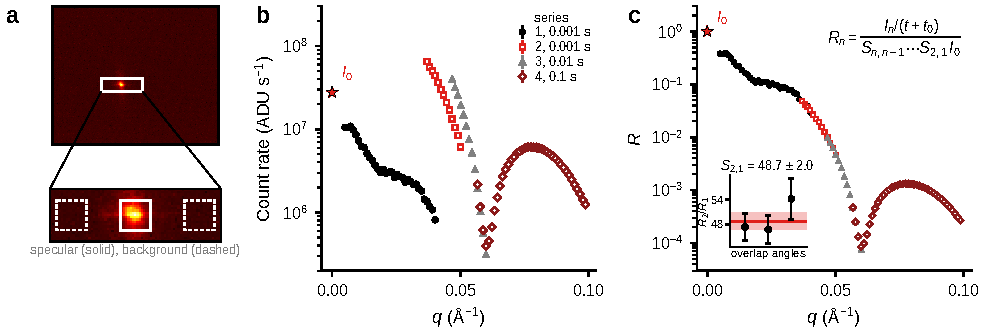
\includegraphics[width=\linewidth,height=0.75\textheight,keepaspectratio]{fig2-09_reduction}
  \caption[Reduction of measured CCD frames into a stitched reflectivity curve, ZnPc at 285.0 eV in s polarization (Scan 85302).]{Reduction of measured CCD frames into a stitched reflectivity curve, ZnPc at 285.0 eV in s polarization (Scan 85302). a) A 2 × 2 binned frame at θ = 13.56° and 0.1 s on a logarithmic scale, with the specular region enlarged. Specular counts are summed in a 13 × 13 pixel box (solid), and the background is the mean of two equal boxes 28 pixels to either side (dashed). b) Background-subtracted count rate, counts divided by the exposure t plus the shutter offset t0 = 3.9 ms, for the four series and the direct beam I0 (star). Each series has its own exposure and higher-order suppressor position and repeats the last angles of the previous series. c) Stitched reflectivity with propagated uncertainties, mostly smaller than the markers, each series divided by I0 and by the running product of stitch factors Sn,n−1. Inset, R2/R1 at the overlap angles and S2,1 = 48.7 ± 2.0 with its uncertainty (red band).}
  \label{fig:3.5}
\end{figure}


Figure~\ref{fig:3.5} follows one measured scan through this reduction, a ZnPc film at 285.0 eV in s polarization collected on the CCD detector. On each frame the specular beam is summed in a fixed box and the background is estimated from two boxes of equal size on either side of it (Fig.~\ref{fig:3.5}a). Dividing the background-subtracted counts by the effective exposure \(t + t_{0}\) converts each frame to a count rate. The shutter offset \(t_{0}\) = 3.9 ms is nearly four times the 1 ms exposure of the first two series, the limit of the original shutter, so it cannot be neglected. The resulting count rates fall into four disjoint series (Fig.~\ref{fig:3.5}b). Within a series the rate follows the reflectivity, but at each series boundary the higher-order suppressor is withdrawn or the exposure lengthened, with the rate jumping by a factor that must be measured rather than taken from the nominal attenuation. The overlap angles provide that measurement. Each new series repeats the last few angles of the previous one, and the stitch factor \(S_{n,n - 1}\) is the slope of an orthogonal-distance regression of \(R_{n} = SR_{n - 1}\) through the origin on those angles (Fig.~\ref{fig:3.5}c, inset), as detailed below. Dividing the first series by the direct beam \(I_{0}\), and each later series by \(I_{0}\) and the running product of stitch factors, yields a single reflectivity curve spanning more than three decades in the first 0.10 Å\(^{- 1}\) (Fig.~\ref{fig:3.5}c). The stitch factors for this scan are \(S_{2,1} = 48.7 \pm 2.0\), \(S_{3,2} = 3.05 \pm 0.04\), and \(S_{4,3} = 1.13 \pm 0.03\). Their uncertainties enter every point of the later series as a common scale error, which a point-by-point uncertainty does not capture and which the error budget below identifies as a correlated term. The reduction shown here omits the dezinger and median filters and the beam-current normalization of the production code, pxr-reduce,\autocite{alsrsoxspxrreduce2026als} which implements the full routine described above.

\subsection{Stitching Details}\label{stitching-details}

Each series after the first opens by repeating the last angles of the series before it, and these overlap angles fix the relative scale of the two series (Fig.~\ref{fig:3.5}c, inset). Repeated frames at the first angle of a new series are excluded, and the remaining overlap angles \(k\) give paired reflectivities \(R_{n - 1,k}\) and \(R_{n,k}\), both normalized by the same \(I_{0}\) but recorded at different higher-order suppressor positions or exposure times. The stitch factor \(S_{n,n - 1}\) is the slope of the line \(R_{n,k} = S_{n,n - 1}R_{n - 1,k}\) through the origin, found by orthogonal distance regression\autocite{boggs1990orthogonal}, which minimizes the summed squared perpendicular distances of the overlap points from the line. Both series carry comparable counting noise at the overlap, and an ordinary least-squares fit, which assigns all of the scatter to the ordinate, would bias the slope low through the noise in the abscissa. The standard error of \(S_{n,n - 1}\) is taken from the covariance of the regression scaled by its residual variance, so it reflects the observed scatter of the overlap points rather than an assumed noise model. Series \(n\) is then placed on the scale of the first series by the running product of stitch factors, \(R_{n} = r_{n}/\left( I_{0}\prod_{m = 2}^{n}S_{m,m - 1} \right)\), where \(r_{n} = I_{n}/\left( t + t_{0} \right)\) is the background-subtracted count rate. The procedure follows pxr-reduce, with the reduction of Fig.~\ref{fig:3.5} performing the regression with the ODR module of SciPy.\autocite{virtanen2020scipy,alsrsoxspxrreduce2026als}

\subsection{Accounting for Measurement Uncertainty}\label{accounting-for-measurement-uncertainty}

Traditional modes of accounting for photon measurement errors originate with the standard counting (shot) noise that scales as the square root of the number of measured events. This assumes that the probability of an individual event does not depend on the number of events already measured. Under this approach the variance of a measured number of counts \emph{N} is \emph{N} itself.

This per-count shot noise propagates in quadrature through each step of the reduction routine above. The row-by-row and column-by-column background corrections each contribute an independent variance from the subtracted background estimate, and the subsequent background-region subtraction adds a further, independent term of the same form. Summed in quadrature, the total variance carried into each measured specular intensity is the sum of the counting variance, the row and column background variance, and the background-region variance, each following ordinary Poisson counting statistics before the detector\textquotesingle s own response is considered.

The uncertainty of each stitched point combines independent and shared terms. For \(R_{n}\) as above, the relative variance is \(\sigma_{R}^{2}/R^{2} = \sigma_{r}^{2}/r^{2} + \sigma_{I_{0}}^{2}/I_{0}^{2} + \sum_{m = 2}^{n}\sigma_{S,m}^{2}/S_{m,m - 1}^{2}\), where \(\sigma_{r}\) combines the counting variance of the specular box with the variances of the row, column, and region background estimates, and \(\sigma_{I_{0}}\) is the scatter of the repeated direct-beam frames. The first term changes from point to point. The last two are shared by every point of a series, so in a fit they act as a correlated scale error rather than as independent point uncertainties, although Fig.~\ref{fig:3.5} adds them in quadrature to each point as the reduction convention. For the scan of Fig.~\ref{fig:3.5} the stitch factors are \(S_{2,1} = 48.7 \pm 2.0\), \(S_{3,2} = 3.05 \pm 0.04\), and \(S_{4,3} = 1.13 \pm 0.03\), so the 4 percent uncertainty of the first stitch dominates the scale of every later series.

The detector records analog to digital units (ADU)\autocite{gann2012soft} a value that is proportional to the number of electrons generated within each pixel, with electron generation in turn proportional to the number of incident photons. The quantum efficiencies of the detector along with the gain set the photon-electron conversion rates, while the internal circuitry sets the conversion from electrons to recorded ADUs displayed on the detector. Notably the quantum efficiency and gain are independent of absolute intensity, yet the electron-ADU conversion depends on the number of electrons within each pixel well. The variance of the number of electrons generated per absorbed photon is also smaller than the Poisson value, by the Fano factor, which quantifies the sub-Poissonian suppression of variance in electron-hole pair generation. In practice this detector-level contribution is small next to the counting and background terms above and is neglected in the error budget below.

The dominant remaining source of uncertainty, however, is not detector noise but the ambiguity in separating the specular beam from off-specular diffuse scattering at high incident angle, where the two become difficult to resolve on a finite-sized detector. Chapter 4\textquotesingle s Methods addresses this directly with an empirical envelope term added in quadrature to the propagated counting uncertainty (Eq. 5), which dominates the reported uncertainty at high \emph{q}. The envelope is itself a model of the measurement error, and like the structural model it can be tested against the data and refined, for example by fitting its coefficients together with the structure.

\section{Analysis Methods}\label{analysis-methods}

Analysis of a reflectivity dataset couples a forward model, which computes the reflectivity of a parameterized film exactly, with an optimizer that adjusts the parameters to minimize the misfit to the data. A posterior estimate then converts the optimum into parameter uncertainties. Competing models are then compared by criteria that penalize added complexity. The sections below treat each stage in turn with the ZnPc film of Chapter 4 as the running example. Each stage is implemented in open-source packages, refloxide for the forward model and refnx for objectives, fitting, and sampling.\autocite{nelson2019textless,alsrsoxsrefloxide2026als}

\subsection{Simulating Reflectivity}\label{simulating-reflectivity}

All reflectivity in this dissertation is computed with refloxide, a 4 × 4 transfer matrix engine for polarized reflectivity from stratified media developed as part of this work.\autocite{alsrsoxsrefloxide2026als} For isotropic layers the reflectivity follows from the Parratt recursion at negligible cost, with well-tested implementations available.\autocite{parratt1954surface,nelson2019textless} For anisotropic layers each slab requires an eigendecomposition and a chain of 4 × 4 matrix products, and a resonant dataset repeats this for every energy, polarization, and angle measured, so the forward model dominates the cost of a fit. refloxide therefore places the calculation in a Rust core with thin Python bindings, offers an optional GPU path through wgpu, and plugs into refnx for modeling and fitting, so that a model spanning many energies remains practical inside an optimizer loop.

Near the critical angle the reflected amplitude is not small, and at every buried interface part of the field is reflected back into the film, reflected again at the interface above, and returned toward the detector with a phase set by the round trip (Fig.~\ref{fig:3.6}a). The transfer matrix method accounts for every such order exactly. Within each layer the field vector \(\Psi = \left( E_{x},H_{y},E_{y}, - H_{x} \right)^{\mathsf{T}}\) obeys \(\partial_{z}\Psi = i(\omega/c)\Delta\Psi\), where \(\Delta\) is the 4 × 4 Berreman matrix built from the local dielectric tensor\autocite{berreman1972optics,passler2017generalized,passler2019generalized}, whose eigenmodes define the interface matrices \(L_{i}\) and the propagation matrices \(P_{i}\). Their ordered product \(\Gamma_{N} = L_{1}P_{1}L_{2}P_{2}\cdots L_{N}P_{N}L_{N + 1}\) maps the field across the whole stack, and the reflectivities follow as \(R_{kl} = \left| r_{kl}\left( \Gamma_{N} \right) \right|^{2}\), valid because the incident medium is isotropic\autocite{yeh1980optics}. The isotropic limit reduces to the Parratt recursion,\autocite{parratt1954surface} and the anisotropic form is the one used for resonant reflectivity of oriented organic films\autocite{capelli2019quantitative,pasquali2014structural,pasquali2021analysis} and implemented in refloxide. Figure~\ref{fig:3.6}b to d compares this result with the kinematic approximation, which retains one reflection per interface, for three stacks at 285.1 eV. For the single ZnPc film of Chapter 4 (Fig.~\ref{fig:3.6}b) the kinematic curve exceeds unity below the critical angle and misplaces and deepens the first minima, although at higher \(q\) it reproduces the fringe spacing \(2\pi/t \approx 0.033\) Å\(^{- 1}\). For the edge-on over face-on bilayer (Fig.~\ref{fig:3.6}c) the agreement is closer, with a median deviation of 0.13 decades, but the kinematic model distorts the low-\(q\) fringes and drives the minimum near 0.18 Å\(^{- 1}\) below \(10^{- 8}\). In the six-period multilayer (Fig.~\ref{fig:3.6}d) both models place the Bragg peaks of the 80 Å period near 0.079 and 0.236 Å\(^{- 1}\), but below the first peak the kinematic model predicts sharp oscillations that multiple reflections damp and redistribute, with the median deviation reaching 0.31 decades. The kinematic errors are largest near the critical angle and at the deep minima, the regions that carry much of a fit\textquotesingle s sensitivity to density and interfacial structure (Fig.~\ref{fig:3.8}),so every simulation in this dissertation uses the transfer matrix.

\begin{figure}[tbp]
  \centering
  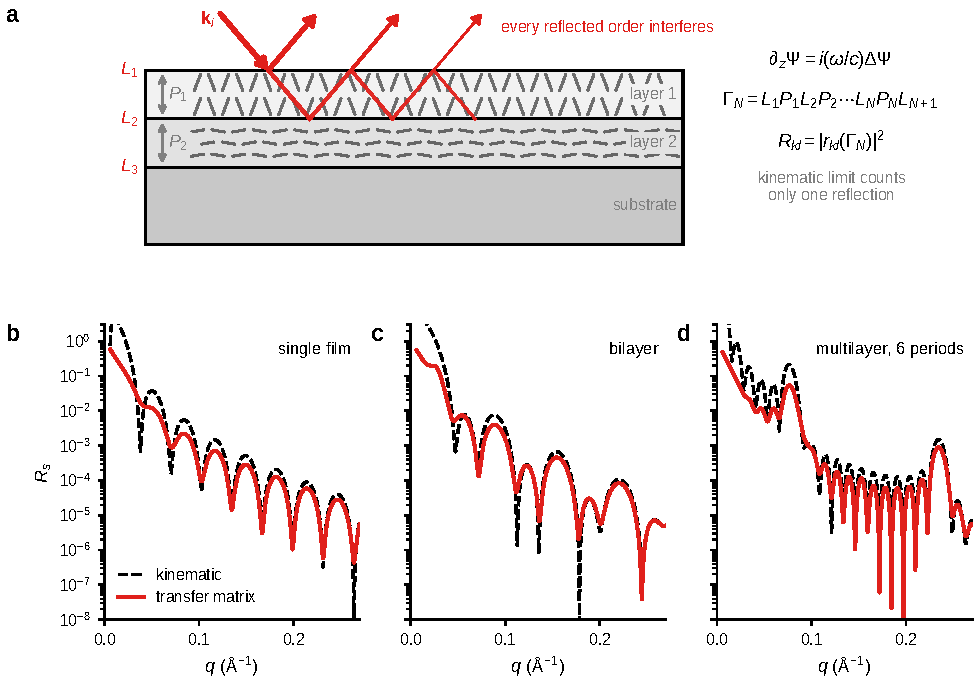
\includegraphics[width=\linewidth,height=0.75\textheight,keepaspectratio]{fig2-11_transfer-matrix}
  \caption[Multiple reflections make the exact solution of the layer stack necessary.]{Multiple reflections make the exact solution of the layer stack necessary. a) Every interface of a stack with edge-on (layer 1) and face-on (layer 2) molecules reflects and transmits, and all reflected orders interfere at the detector. The field vector Ψ obeys ∂zΨ = i(ω/c)ΔΨ in each uniaxial layer, and interface matrices Li and propagation matrices Pi compose to the stack matrix ΓN that gives the reflection coefficients. b to d) s-polarized reflectivity at 285.1 eV from the transfer matrix (red) and the kinematic approximation (black, dashed) for the Chapter 4 single film (b), a 100 Å edge-on layer over a 90 Å face-on layer (c), and six periods of 40 Å edge-on and 40 Å face-on layers (d). The median deviation between the two is 0.23, 0.13, and 0.31 decades for b, c, and d.}
  \label{fig:3.6}
\end{figure}


\begin{figure}[tbp]
  \centering
  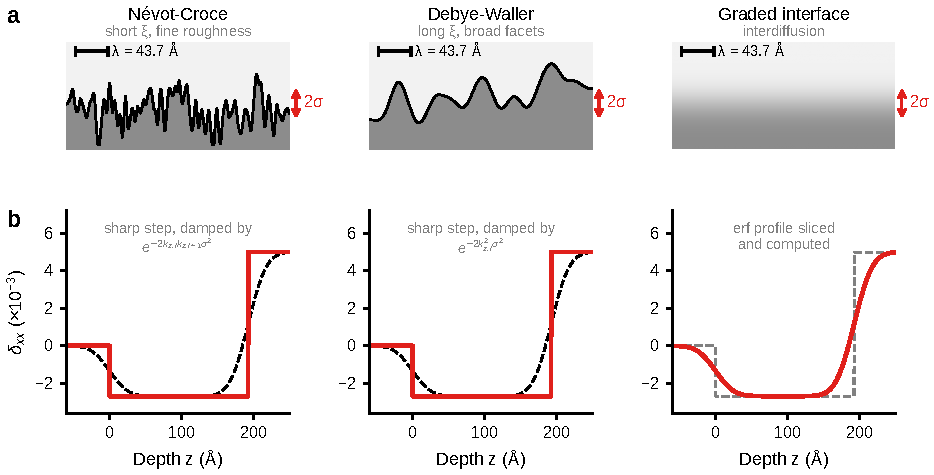
\includegraphics[width=\linewidth,height=0.75\textheight,keepaspectratio]{fig2-12_interfaces}
  \caption[Three interface models at the same roughness σ = 20 Å for a 192.7 Å ZnPc film on Si at 283.7 eV.]{Three interface models at the same roughness σ = 20 Å for a 192.7 Å ZnPc film on Si at 283.7 eV. a) Real-space interfaces drawn at equal lateral and vertical scale, with the wavelength λ = 43.7 Å and 2σ (red) marked. Névot-Croce describes fine roughness with a short in-plane correlation length ξ, Debye-Waller describes broad facets with a long ξ, and the graded interface describes interdiffusion without in-plane structure. b) Depth profiles of δxx as each model computes them. Névot-Croce and Debye-Waller compute the sharp profile (red), shown with the error-function profile usually drawn for them (black, dashed), while the graded interface slices the error-function profile into 1 Å layers and computes it directly (red), with the sharp profile for reference (gray, dashed).}
  \label{fig:3.7}
\end{figure}


Real interfaces are neither flat nor sharp. The three models in common use differ in what they assume about an interface and in where that assumption enters the calculation (Fig.~\ref{fig:3.7}). Névot-Croce and Debye-Waller roughness both keep the computed depth profile sharp and multiply each interface Fresnel coefficient by a damping factor, \(\exp\left( - 2k_{z,i}k_{z,i + 1}\sigma^{2} \right)\) for Névot-Croce\autocite{nevot1980caracterisation} and \(\exp\left( - 2k_{z,i}^{2}\sigma^{2} \right)\) for Debye-Waller\autocite{deboer1996x,holy1993x}. The error-function profile usually drawn for these models (Fig.~\ref{fig:3.7}b, dashed) is a display convention that the calculation never uses, so the two models share one depth profile and differ only in the reflectivity they predict. The damping factors encode different interfaces. Névot-Croce assumes fine roughness with an in-plane correlation length \(\xi\) short compared with \(\xi_{diff} = \lambda/(1 - cos\theta)\), whereas Debye-Waller assumes broad facets with \(\xi\) long compared with \(\xi_{diff}\) (Fig.~\ref{fig:3.7}a). At 283.7 eV, \(\xi_{diff}\) falls from about \(10^{4}\) Å at \(\theta\) = 5° to about 300 Å at \(\theta\) = 30°, so the appropriate factor can change within a single scan and depends on lateral structure that specular reflectivity does not measure. The graded interface makes no claim about lateral structure. It slices the error-function profile into 1 Å layers and propagates the field through each one, so the depth profile is the computed one (Fig.~\ref{fig:3.7}b, right). This is the appropriate description of interdiffusion and of real composition or orientation gradients, serving as the reference for the multiplicative models. At \(\sigma\) = 20 Å the s-polarized reflectivity from the Névot-Croce and Debye-Waller factors departs from the graded result by up to 28 and 51 percent below \(q\) = 0.15 Å\(^{- 1}\), so at large roughness the factors are approximations to be tested against the graded model, consistent with numerical comparisons of these roughness treatments for X-ray and extreme-ultraviolet reflectance.\autocite{esashi2021influence} The refloxide selection guide states these regimes in terms of \(\sigma k_{z}\) and \(\xi/\xi_{diff}\).\autocite{alsrsoxsrefloxide2026als} In Chapter 4 the slab model applies Névot-Croce roughness at each interface, while the depth gradient is a physically motivated multi-slice profile of molecular tilt and density, computed slice by slice in the same way as the graded interface.

The graded interface is one case of a general multi-slice description, in which any depth profile of the optical tensor is discretized into slabs thin compared with \(\pi/q_{z,max}\) and each slab is assigned its own tensor. A composition gradient varies the density of each component across the slices, and an orientation gradient varies the tilt \(\gamma\) entering the film tensor of Chapter 2, so that \(n_{xx}^{f}(z)\) and \(n_{zz}^{f}(z)\) change independently with depth. The exponential profiles of the orientation gradient section enter the Chapter 4 model in this way. The slice thickness should be chosen so that halving it changes the computed reflectivity by less than the measurement uncertainty.

\subsection{Fitting Polarized Reflectivity}\label{fitting-polarized-reflectivity}

The goal of the resonant scattering experiment is to uncover physical structures and size scales along with the molecular states within these structures, but there are no general direct inversion algorithms to uncover both properties. Because scattering intensity is measured in the far field regime, it arises from the Fourier transform of the near field projection, with much of the near-field information lost because only intensity is measured. As a direct consequence, the only way to quantitatively uncover both properties follows an inverse problem. A model and parameter set are chosen and used to simulate the experimental scattering, after which the parameters are refined to fit the data. But this requires the user to choose a good model that can describe the underlying structures and molecular states along with a good choice in parameterization that sufficiently removes covariance and degeneracies. Yet even for good choices, there is no guarantee of solution uniqueness, since multiple models and parameterization choices can result in statistically identical simulated scattering intensities.

Because of this, it is the job of the researcher to identify the most likely model based on physical and chemical properties and other experimental results. Prior chemical knowledge, such as the expected film stoichiometry or known crystallographic phases, together with auxiliary measurements like GIXRD or ellipsometry, constrains this choice before any fitting begins. These constraints enter a fit as fixed parameters, such as the optical constants of the substrate, as bounds that exclude unphysical densities or thicknesses, and as joint fits in which one structure must describe several energies and polarizations at once. The joint fit is the strongest of these, and it is the constraint that the physically constructed optical tensors of Chapters 4 and 5 make available.

\begin{figure}[tbp]
  \centering
  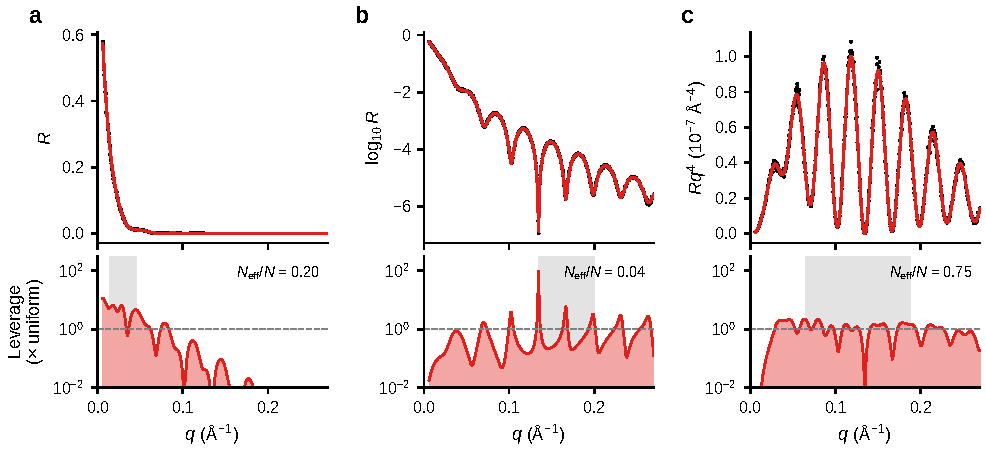
\includegraphics[width=\linewidth,height=0.75\textheight,keepaspectratio]{fig2-13_objective-transforms}
  % TODO caption contains equations that were flattened to plain text in the Word export; retypeset them.
  \caption[Objective transforms change which points control a reflectivity fit.]{Objective transforms change which points control a reflectivity fit. A simulated s-polarized dataset for the Chapter 4 ZnPc film at 285.1 eV, with noise σ=aR+bq (points) and the model (red), shown as a) R, b) log10R, and c) Rq4. Below each panel is the statistical leverage of every point in an unweighted least-squares fit of film thickness, roughness, tilt, and density, relative to a uniform share (dashed line). Neff/N is the participation ratio, the fraction of points that effectively carry the fit.}
  \label{fig:3.8}
\end{figure}


\subsection{Objective Transforms - linearization}\label{objective-transforms---linearization}

An unweighted least-squares objective counts every point equally in whatever representation the data are fit, so the representation decides which points control the fit. Figure~\ref{fig:3.8} shows one simulated dataset, the Chapter 4 film at 285.1 eV with noise \(\sigma = aR + bq\), as \(R\), \(\log_{10}R\), and \(Rq^{4}\) (Fig.~\ref{fig:3.8}a to c). Below each panel is the statistical leverage of every point, the diagonal of the hat matrix \(\mathbf{J}\left( \mathbf{J}^{\mathsf{T}}\mathbf{J} \right)^{- 1}\mathbf{J}^{\mathsf{T}}\) for film thickness, roughness, tilt, and density, relative to a uniform share (dashed line). Leverage measures how strongly the fitted model is pulled toward each point, with its participation ratio \(N_{eff}/N\) giving the fraction of the dataset that effectively carries the fit. On a linear scale the critical-angle region dominates, with the central half of the leverage between \(q\) = 0.014 and 0.046 Å\(^{- 1}\) (\(N_{eff}/N\) = 0.20). The logarithm spreads weight across the decades but concentrates it at the fringe minima, where a small shift in fringe position changes \(\log R\) by orders of magnitude. The deep minimum near 0.135 Å\(^{- 1}\) alone carries 93 times a uniform share (\(N_{eff}/N\) = 0.04). Multiplying by \(q^{4}\) removes the Fresnel decay, so the leverage stays close to the uniform share across most of the range, never exceeding 2.2 times it, with three quarters of the points contributing effectively (\(N_{eff}/N\) = 0.75). With correctly propagated uncertainties the choice matters little, since \(\sigma_{\log R} = \sigma_{R}/\left( R\ln 10 \right)\) and to first order every representation yields the same weighted \(\chi^{2}\). It matters when uncertainties are absent, underestimated, or replaced by uniform weights. Because each transform also changes the implied distribution of the noise, the representation is part of the statistical model and is reported with it. Both transforms are available as objective transforms in refnx\autocite{nelson2019textless} and are used in this dissertation. The fits of Chapter 4 and the ZnPc comparison of Chapter 5 use \(\log R\), while the Alq\(_{3}\) fits of Chapter 5 use \(Rq^{4}\).

\subsection{Optimizers}\label{optimizers}

Reflectivity objectives combine three difficulties, isolate in Fig.~\ref{fig:3.9} on a two-parameter problem. The Kiessig fringes make the objective sharp and periodic, since a few ångströms of thickness move every fringe. The total optical path of the film is well determined while its division between layers is not, which correlates the parameters into long, narrow, tilted valleys. Fringe aliasing repeats those valleys wherever the model fringes fall on the data fringes shifted by whole periods, each valley a local minimum. The surface in Fig.~\ref{fig:3.9} is built from simulated s- and p-polarized data for the Chapter 4 film with its buriedinterfacial layer, with every optimizer starts from the same point, 17 Å and 15 Å from the true thicknesses. Levenberg-Marquardt, which interpolates between Gauss-Newton and gradient descent,\autocite{marquardt1963algorithm,levenberg1944method} and L-BFGS-B, which builds a limited-memory quasi-Newton Hessian within box bounds,\autocite{byrd1995limited} both descend into the nearest valley and stop at (210.4 Å, 14.1 Å) with \(\log_{10}\chi_{\nu}^{2} = 1.52\), after 69 and 48 evaluations (Fig.~\ref{fig:3.9}a,b). Differential evolution needs no starting point.\autocite{storn1997differential} It evolves a population across the bounded space by mutation and crossover, and by generation 39 the population has collapsed onto the global minimum at (178.0 Å, 15.0 Å), \(\log_{10}\chi_{\nu}^{2} = - 0.58\), at a cost of 984 evaluations (Fig.~\ref{fig:3.9}c). A random-walk Metropolis chain\autocite{metropolis1953equation} also reaches the minimum from this start, but in the sharp valley it accepts only 1 percent of its proposals, so 4000 steps yield few independent samples (Fig.~\ref{fig:3.9}d). We expect a chain started in another valley to cross into this one rarely, which is the mixing problem of naive MCMC on reflectivity objectives.\autocite{machida2024development} Local methods are therefore fast and precise only inside the correct basin, global methods find that basin at 14 to 20 times the cost. Sampling methods are best used to characterize a basin once it has been found. The Chapter 4 workflow follows this order, with differential evolution as the global stage and L-BFGS-B as the local polish.

\begin{figure}[tbp]
  \centering
  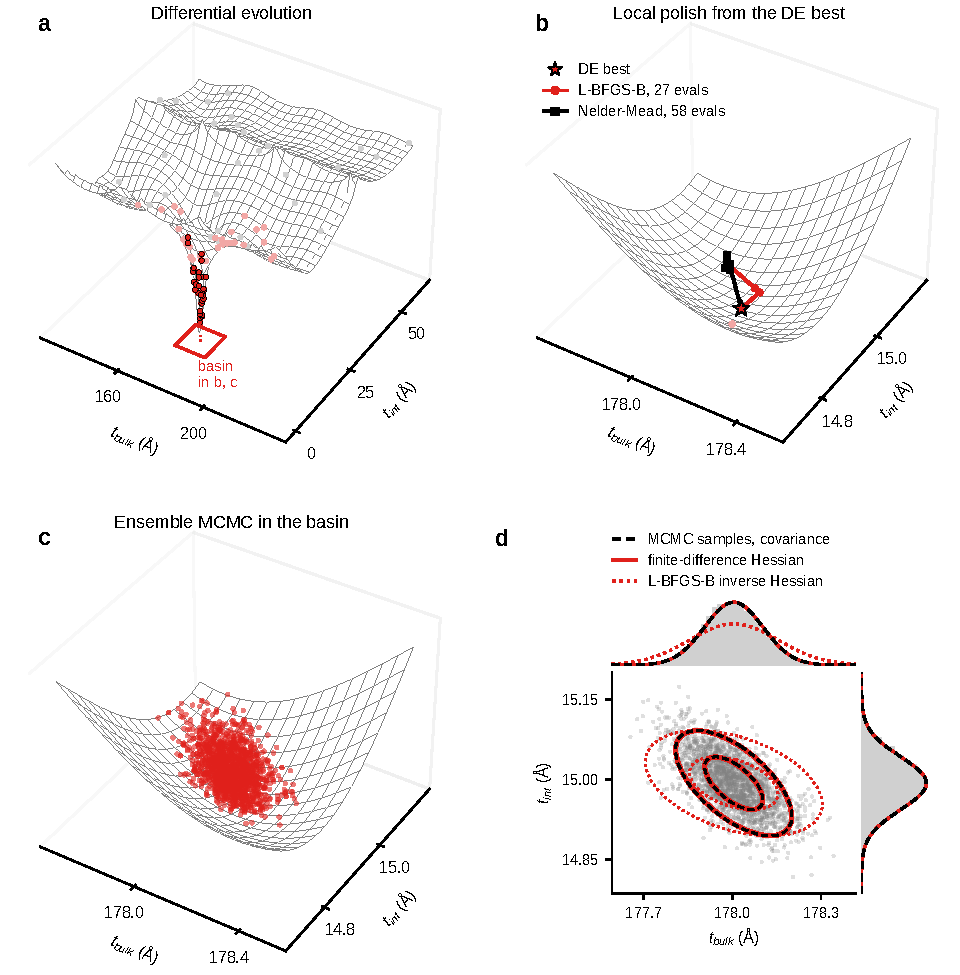
\includegraphics[width=\linewidth,height=0.75\textheight,keepaspectratio]{fig2-15_uncertainty}
  \caption[From the global optimum to parameter uncertainty on the Fig.]{From the global optimum to parameter uncertainty on the Fig.~\ref{fig:3.9} objective. a) Differential evolution with the population at generations 0 (gray), 4 (light red), and 8 (red), reaching (178.2 Å, 14.9 Å) after 270 evaluations. The red box marks the basin enlarged in b and c. b) The log10χ2ν surface over that basin (0.83 Å by 0.46 Å) with the differential-evolution best point (star) and the local polish by L-BFGS-B (red, 27 evaluations) and Nelder-Mead (black, 58 evaluations), both converging to (178.00 Å, 14.99 Å). c) Affine-invariant ensemble MCMC in the same window, 32 walkers for 3000 steps after 1000 steps of burn-in, with an acceptance fraction of 0.72. d) Posterior samples with marginal distributions and 1σ and 2σ contours from the MCMC covariance (black, dashed), the finite-difference Hessian at the minimum (red), and the L-BFGS-B inverse Hessian (red, dotted).}
  \label{fig:3.10}
\end{figure}


\begin{figure}[tbp]
  \centering
  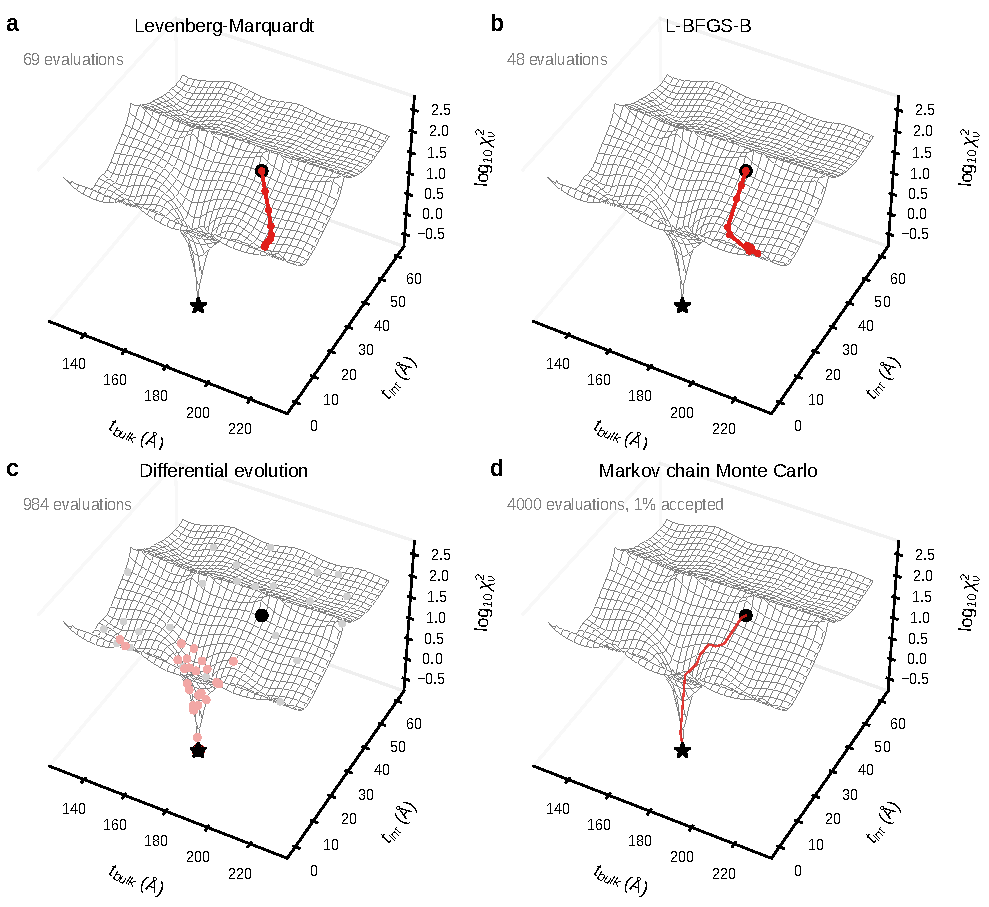
\includegraphics[width=\linewidth,height=0.75\textheight,keepaspectratio]{fig2-14_optimizers}
  \caption[Four optimizers on the same sharp, correlated, and nonlinear reflectivity objective.]{Four optimizers on the same sharp, correlated, and nonlinear reflectivity objective. The surface is log10χ2ν of simulated s- and p-polarized reflectivity at 283.7 eV for the Chapter 4 film divided into a bulk layer of thickness tbulk and a buried interfacial layer of thickness tint, fit on log R, with a single deep minimum (star) at tbulk = 178 Å and tint = 15 Å. Every run starts from the same point (black circle, 195 Å, 30 Å). a, b) Levenberg-Marquardt (69 evaluations) and L-BFGS-B (48 evaluations) descend into the nearest valley and stop at the same local minimum, (210.4 Å, 14.1 Å) with log10χ2ν = 1.52. c) Differential evolution population at generations 0 (gray), 4 (light red), and 39 (red), which converges to the global minimum (178.0 Å, 15.0 Å) with log10χ2ν = −0.58 after 984 evaluations. d) Random-walk Metropolis chain of 4000 steps at the true likelihood, which reaches the minimum from this start but accepts 1 percent of its proposals in the sharp valley.}
  \label{fig:3.9}
\end{figure}


\subsection{Posterior Estimation}\label{posterior-estimation}

Figure~\ref{fig:3.10} completes the workflow on the same objective by converting the global optimum into a parameter uncertainty. Differential evolution locates the basin (Fig.~\ref{fig:3.10}a), but its population carries no curvature information, so it returns a best point without an error estimate. A local optimizer started from that point refines it, and L-BFGS-B and the derivative-free Nelder-Mead method converge to the same minimum at (178.00 Å, 14.99 Å) in 27 and 58 evaluations (Fig.~\ref{fig:3.10}b). Within this basin the objective is close to quadratic, the regime in which affine-invariant ensemble MCMC,\autocite{goodman2010ensemble} as implemented in emcee and refnx\autocite{nelson2019textless}, samples efficiently. Thirty-two walkers accept 72 percent of their proposals (Fig.~\ref{fig:3.10}c), against 1 percent for the random-walk chain on the full surface of Fig.~\ref{fig:3.9}d. The samples give \(\sigma\left( t_{bulk} \right)\) = 0.099 Å and \(\sigma\left( t_{int} \right)\) = 0.050 Å with a correlation of \(- 0.63\) (Fig.~\ref{fig:3.10}d), and the inverse of the finite-difference Hessian at the minimum reproduces these values to within 0.001 Å, as expected for a quadratic basin. The inverse Hessian reported by L-BFGS-B does not. It overstates \(\sigma\left( t_{bulk} \right)\) at 0.150 Å and understates the correlation at \(- 0.40\), because L-BFGS-B builds its Hessian estimate from the few steps it takes, which are few for a run started near the minimum. The internal estimate of a quasi-Newton optimizer is therefore a starting point to be checked against a sampled posterior or a Hessian computed at the minimum. Where the posterior has separated modes, as on the full surface of Fig.~\ref{fig:3.9}, nested sampling as implemented in dynesty\autocite{speagle2020dynesty} is the appropriate extension, since it explores separated modes and returns the evidence used for model comparison in the section that follows. Other approaches such as neural posterior estimation and Bayesian optimization are other approaches to resolve this.\autocite{starostin2025fast,machida2024development}

\subsection{Model Selection}\label{model-selection}

The default statistical test for evaluating model performance considers only the closeness between a model and the data it aims to fit. This is best characterized by the reduced \(\chi^{2}\) statistic that measures this directly. However, this assumes Gaussian, locally linear errors and penalizes nothing for added model complexity, so it cannot by itself discriminate between parameterizations of different dimensionality when the noise is closer to Poissonian and the forward model is nonlinear, as is generically the case for reflectivity.

Other evaluation criteria instead compare models directly against each other. The Bayesian and Akaike information criteria (BIC, AIC) approximate, respectively, the weight of evidence for a model and its expected predictive performance on new data, penalizing additional free parameters so a better fit is only rewarded if it earns its added complexity. Both remain asymptotic approximations, however, and the most direct test of generalization is a validation hold-out, fitting to a subset of the measured energies or angles and scoring the fit against the remainder, which catches overfitting that an information criterion can only estimate.

\subsection{Bayesian Optimization and Amortized Inference}\label{bayesian-optimization-and-amortized-inference}

Bayesian optimization and amortized inference reduce the number of forward evaluations a fit requires rather than improving the search itself. Bayesian optimization fits a Gaussian-process surrogate to the objective and chooses each next evaluation by an acquisition function that balances the predicted objective against its uncertainty.\autocite{noack2021gaussian} It pays off when one forward evaluation is expensive, as for a finite-element solve or a model spanning many energies, and when the number of parameters is small. It is the same machinery proposed for measurement selection in the future-work section. Prior-amortized neural posterior estimation instead trains a normalizing-flow posterior once on simulated reflectivity over a family of priors.\autocite{starostin2025fast} Inference on a new dataset then takes seconds, recovers modes that maximum-likelihood fitting and local MCMC miss, and can be refined by importance sampling or MCMC. Its published demonstrations use isotropic layer models at a single energy. Applying it to the uniaxial models of this work would require training sets simulated with the 4 × 4 transfer matrix at every measured energy and both polarizations, a network conditioned on the energy-dependent tensor of each component or on the parameters that generate it, and a forward model fast enough to make those training sets affordable, which is one motivation for the performance of refloxide.

\section{\texorpdfstring{Future Work }{Future Work }}\label{figmarker19x-figmarker20x-future-work}

\begin{figure}[tbp]
  \centering
  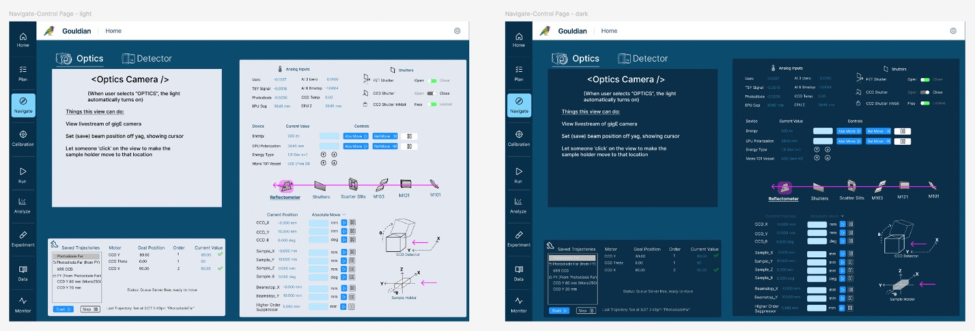
\includegraphics[width=\linewidth,height=0.75\textheight,keepaspectratio]{fig3-11_beamline-ui}
  \caption[Future Beamline 11.0.1.2 beamline user interface (left, light mode, right dark mode).]{Future Beamline 11.0.1.2 beamline user interface (left, light mode, right dark mode). Integrates pan automation, data access and analysis, and a standard control integration to directly drive the beamline.}
  \label{fig:3.11}
\end{figure}


The analysis outlined here is implemented in a Python package co-developed with the beamline staff at the Advanced Light Source.\autocite{alsrsoxspxrreduce2026als} The next step builds the entire measurement process directly into the control systems and drives for the instrument to facilitate the real time reduction and analysis. Importantly, the facility and instruments are in the process of upgrading from a LabVIEW-based control system to a newer expressive system called EPICS. These new EPICS drivers are then integrated directly with Bluesky a common control language used by most other synchrotron facilities and CERN. Bluesky makes it possible to safely write python scripts to control the beamline optics and motors, unlocking the potential for feedback loops and programmatic interaction. Bluesky also integrates with more modern features such as web applications allowing for more standardized UI experience and centralized data storage to unify the experience of collecting and working with data across user facilities. Beamline 11.0.1.2 is currently in the process of upgrading both to use EPICS and Bluesky and a UI/UX refresh that will utilize modern web features such as common authentication and finer-grained, per-user access control (Fig.~\ref{fig:3.11}).

This unlocks direct integration into decision making algorithms such as gaussian process (GP) routines so that new configurations can be algorithmically selected based on the uncertainties in the measured signal, completely removing the need for pre-defined human input such as defining the energy measurement grid. Using a gaussian process has been highly effective in reducing the number of measurements needed to fully capture experimental data, outcompeting uniform grid searches, human decision making and random grids, while also allowing for domain specific and model specific information injection.\autocite{du2025demonstration,alghalayini2025machine} The general idea is to use direct feedback algorithms to automate both the alignment routines and the single condition measurements, while the GP algorithm is used to set a stopping condition on the measurement grid, asserting that each measurement condition (polarization and energy) is fully specified. The next approach then directly integrates the materials film structure into the decision-making process, from the fit performance, using Bayesian optimization (BO) the stopping condition is no longer when the reflectivity is fully specified but when the film's depth profile is fully determined. In this final approach the user of the facility no longer needs to perform the primary reflectivity analysis on their films after their experiment is done, and instead they return home with the depth profile itself allowing their work to focus on uncovering material properties, structure property relationships in functionalized applications, and revealing new phenomena within novel materials.

Figure~\ref{fig:3.12} assembles the procedures of this chapter into the decision loop planned for beamline 11.0.1.2 once its EPICS and Bluesky controls are in place,\autocite{allan2019blueskytextquotesingle} following the cross-facility approach to autonomous scattering.\autocite{koepp2026toward} A Gaussian process holds the current state of knowledge\autocite{noack2021gaussian} and chooses eitherthe next measurement condition, a combination of polarization, photon energy, and angular range, or the next sample. Both branches pass through an alignment checker that encodes the rules of the alignment section. A change of polarization changes the heat load on the optics, so the loop waits 15 min before checking, with the sample realigned with the scans of Fig.~\ref{fig:3.4} only when it fails a check of the reflected beam at 1° and 2°. A condition is then measured one series at a time. Before each series the incident intensity is raised through the higher-order suppressor and the exposure time, and the series runs until the reflected beam falls below the noise floor, which reproduces the series structure of Fig.~\ref{fig:3.5} without a predefined list of angles. When a condition is complete, control returns to the Gaussian process, whose stopping rule asserts that every polarization and energy has been specified. Replacing that rule with Bayesian optimization on the fit itself would end the measurement when the depth profile, rather than the reflectivity, is determined. The loop remains under development and is outlined here to set the direction rather than to report a result.

\begin{figure}[tbp]
  \centering
  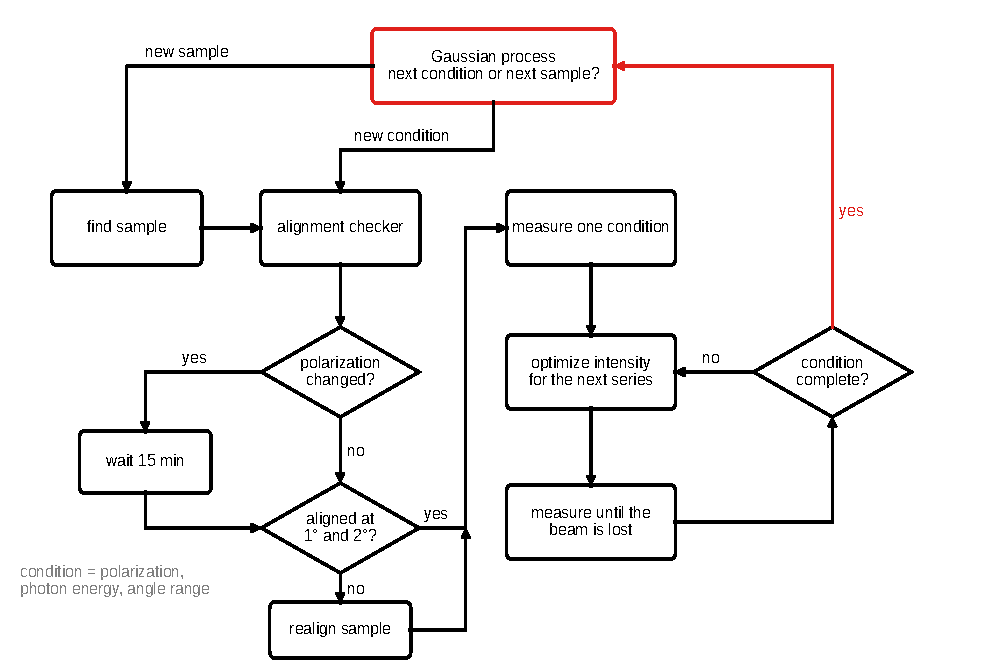
\includegraphics[width=\linewidth,height=0.75\textheight,keepaspectratio]{fig2-16_automation}
  \caption[Decision loop for autonomous reflectivity measurement.]{Decision loop for autonomous reflectivity measurement. A Gaussian process chooses the next condition (polarization, photon energy, and angle range) or the next sample, and a new sample is located before both branches pass to the alignment checker. After a polarization change the loop waits 15 min, and the sample is realigned whenever it fails the check at 1° and 2°. Each condition is measured one series at a time, with the incident intensity optimized for each series and data collected until the beam is lost, and a completed condition (red) returns control to the Gaussian process.}
  \label{fig:3.12}
\end{figure}


\section{Summary}\label{summary}

This chapter has assembled the physical and practical basis on which every later result rests. The detector records only far-field intensity, so the phase and near-field structure of the scattered wave are lost, and every result in this dissertation is therefore obtained by forward modeling the measurement and fitting it. The optical response entering that model is the tensor index \(n = 1 - \delta + i\beta\), with \(\beta\) taken from the mass absorption and \(\delta\) from its Kramers-Kronig transform, so the bare-atom extrapolation of \(\beta\) outside the measured window enters \(\delta\) at every energy. Each resonance contributes to this tensor through its transition dipole, and averaging the uniaxial molecular tensor over the azimuth gives the film tensor as a function of the tilt \(\gamma\) and the density \(\rho\), the two quantities refined in Chapters 4 and 5. The Ginzburg-Landau treatment adds a physical form for how these quantities relax toward the bulk, the exponential depth profiles used for the interfacial gradients of Chapter 4.

The experimental and analysis sections carry this framework into practice. In the measurement, the angular zero is set by a forward-model fit of the rocking scan, because a finite beam and photodiode bias the conventional half-maximum alignment, and the stitch factors that join attenuated series carry a correlated scale uncertainty that a point-by-point error bar does not capture. In the analysis, reflectivity is computed exactly by the transfer matrix, roughness is treated with Névot-Croce factors checked against explicitly graded interfaces, and fits are made on \(\log R\) or \(Rq^{4}\) with the transform reported as part of the noise model, since the transform decides which points control the fit. The global optimum is located by differential evolution, refined with L-BFGS-B, and assigned uncertainties by ensemble MCMC, a sequence suited to the sharp, correlated, and multimodal objectives typical of reflectivity. The chapter closes with the autonomous measurement loop toward which beamline 11.0.1.2 is moving, in which the same forward model decides what to measure next.

\chapter{Sub-monolayer Tracking of Molecular States at Buried Interfaces}\label{chap:znpc}

Prepared for submission to an academic journal.

Harlan Heilman, Em Biegler, Sushil Adhikari, Victor Murcia, Tanner Melody, Fred Woodall, Lars Thomsen, Obaid Alqahtani, and Brian A. Collins, ``Sub-monolayer tracking of molecular states at buried interfaces,'' arXiv:2610.31924 (2026).\autocite{heilman2026sub}

This chapter is adapted from the manuscript above, which is under peer review and posted as a preprint on arXiv. The first question of \cref{chap:introduction} is examined here by applying the film tensor of \cref{chap:molecular-films} and the transfer matrix forward model and fitting workflow of \cref{chap:methods} to polarized resonant reflectivity of ZnPc films on silicon. Figure and table numbers follow the dissertation, with the supporting information in Supplemental Material.

\section{Attributions}\label{sec:attributions}

HH and BAC conceived the study. BAC oversaw and directed all aspects of the study. HH performed RSoXS measurements, DFT calculations, developed and performed the structural and optical modeling, and wrote the manuscript. FW deposited samples measured with RSoXS and performed and measured AFM topology. EB deposited a separate sample, collected, and analyzed non-resonant XRR. SA performed and analyzed VASE. TM collected and analyzed GIWAXS and measured AFM topography. VM assisted with DFT calculations and clustering. LT collected AR-NEXAFS and OA processed and analyzed the AR-NEXAFS.

\section{Introduction}\label{sec:introduction}

The molecular orientation\autocite{tumbleston2014influence,yokoyama2011molecular}, composition\autocite{collins2013absolute} and oxidation state\autocite{cabana2018mechanisms,wang2024insights} at the inaccessible interfaces of buried nanoscale assemblies are decisive quantities that dictate material function across physics, chemistry and materials science critical to advanced technologies. For example, in extreme-ultraviolet photoresists the chemical gradient at the edge of the latent image limits the minimum achievable process size for microprocessors.\autocite{debisschop2017stochastic,andrle2026nanostructure} In organic devices such as solar cells, LEDs, transistors, and spin valves the orientation and conformation of the molecular monolayer at the interface governs emergent electronic states that control charge generation, recombination, transport, and spin hybridization respectively.\autocite{tumbleston2014influence,yokoyama2011molecular,pei2020semiconductor,jiang2025toughened,droghetti2016dynamic} In bio- and chemical sensing, molecular states at buried interfaces have resulted in novel ionic transport dynamics.\autocite{khan2025local,trigg2018self,dong2010super} Controlling molecular states directly at these interfaces is, therefore, central to advancing each of these technologies.

Unfortunately, the few techniques that resolve buried interfacial structure, such as atom probe tomography are laborious, highly destructive, and can't resolve details of bonding states and their orientations.\autocite{cojocarumiredin2024atom} Lacking a direct probe, novel interfacial molecular states (e.g. orientation and packing) are thought to be achieved via substrate patterning effects,\autocite{kato2020morphological,ngongangndjawa2015impact,schunemann2011zinc} similar to atomic epitaxial growth. Studies have attempted to access the buried molecular state by measuring deposition at coverage checkpoints\autocite{derrien2022interfacial,yamamoto2022variation,deoteyza2006structural} with in situ measurements resolving a density stratification that contradict the patterning hypothesis.\autocite{derrien2022interfacial} Yet other work suggests these coverage snapshots only describe the exposed molecular layers in a transient state that change once buried,\autocite{yamamoto2022variation,deoteyza2006structural} leaving the mechanisms governing formation and control of interfacial states unresolved.

RSoXS, tuned to the energies of electronic transitions into unoccupied molecular orbitals can non-destructively reveal the chemical, electronic, and physical states within these buried structures\autocite{grabner2025resonant,andrle2026nanostructure,andrle2025using}. The scattered intensity is determined by two coupled effects, the geometric structure of the assembly and the optical interaction with the material. For reflectivity analysis, models of these effects are fit to scattering data to reveal depth-dependent information.\autocite{grabner2025resonant,ferron2022characterization,wang2007resonant,yan2013accurate,mezger2011molecular,ferron2023composition} Unfortunately, the physio-chemical states must be inferred from of optical parameters as a function of energy and polarization which increase in number for each energy probed, causing the analysis to become unstable. Therefore, analyses retreat to a single diagnostic resonance which cannot distinguish chemical species nor orientation unless simplifying assumptions are made.\autocite{ferron2022characterization,li2026pattern,nguyen2024resonant} Worse, a buried interfacial layer is typically required to accurately fit the data which is assumed to be comprised of contaminants or oxidation,\autocite{ferron2022characterization,wang2007resonant,mezger2011molecular,ferron2023composition} and there is no way to determine if these layers are real or merely a limitation of the soft X-rays' diffraction limit which sets the smallest resolvable feature by the scatterer's wavelength, in this case, several nanometers.

Recently, near edge X-ray absorption fine structure (NEXAFS) spectroscopy measurements have been used to construct an Edisonian optical model, enabling the orientation state to be inferred though a secondary analysis of the optical parameters, although the above limitations remain.\autocite{ferron2022characterization,wang2007resonant,yan2013accurate,ferron2023composition,thelen2020molecular} Alternative approaches arrive at the optical model from density functional theory (DFT), yet are limited by fundamental computational inaccuracies.\autocite{pasquali2014structural,capelli2019quantitative,pasquali2021analysis} Recently, we have demonstrated that ML-refined DFT optical models can quantitatively reproduce angle-resolved (AR) NEXAFS measurements of polycrystalline thin films with different orientation and crystal phases while retaining individual bond identity and orientation.\autocite{murcia2026quantitative}

Here we construct and apply an ML-DFT optical model in RSoXS analysis to directly quantify molecular chemical identity, orientation and density as a function of depth in a molecular thin film. The approach ties spectral resonances together in one physical model of the molecule, to increase chemical and orientational sensitivity, and locks scattering features between energies and polarization to recover lost diffraction limited information. This results in sub-monolayer resolution of molecular chemical andorientational state. Analysis of the bottom interface reveals not contaminants or a substrate patterned crystal phase, but a smooth variation of molecular state with partial coverage of the molecule in a unique orientation and packing state directly at the heterointerface. This discovery establishes the bulk texture is set not by substrate patterning but by competing surface and intermolecular interactions during film growth. The new analysis, therefore, enables direct characterization of buried structures at the molecular level critical to the physics of crystal growth, kinetic deposition, and solvent interaction models that dictate these interfaces across material systems.

\begin{figure}
  \centering
  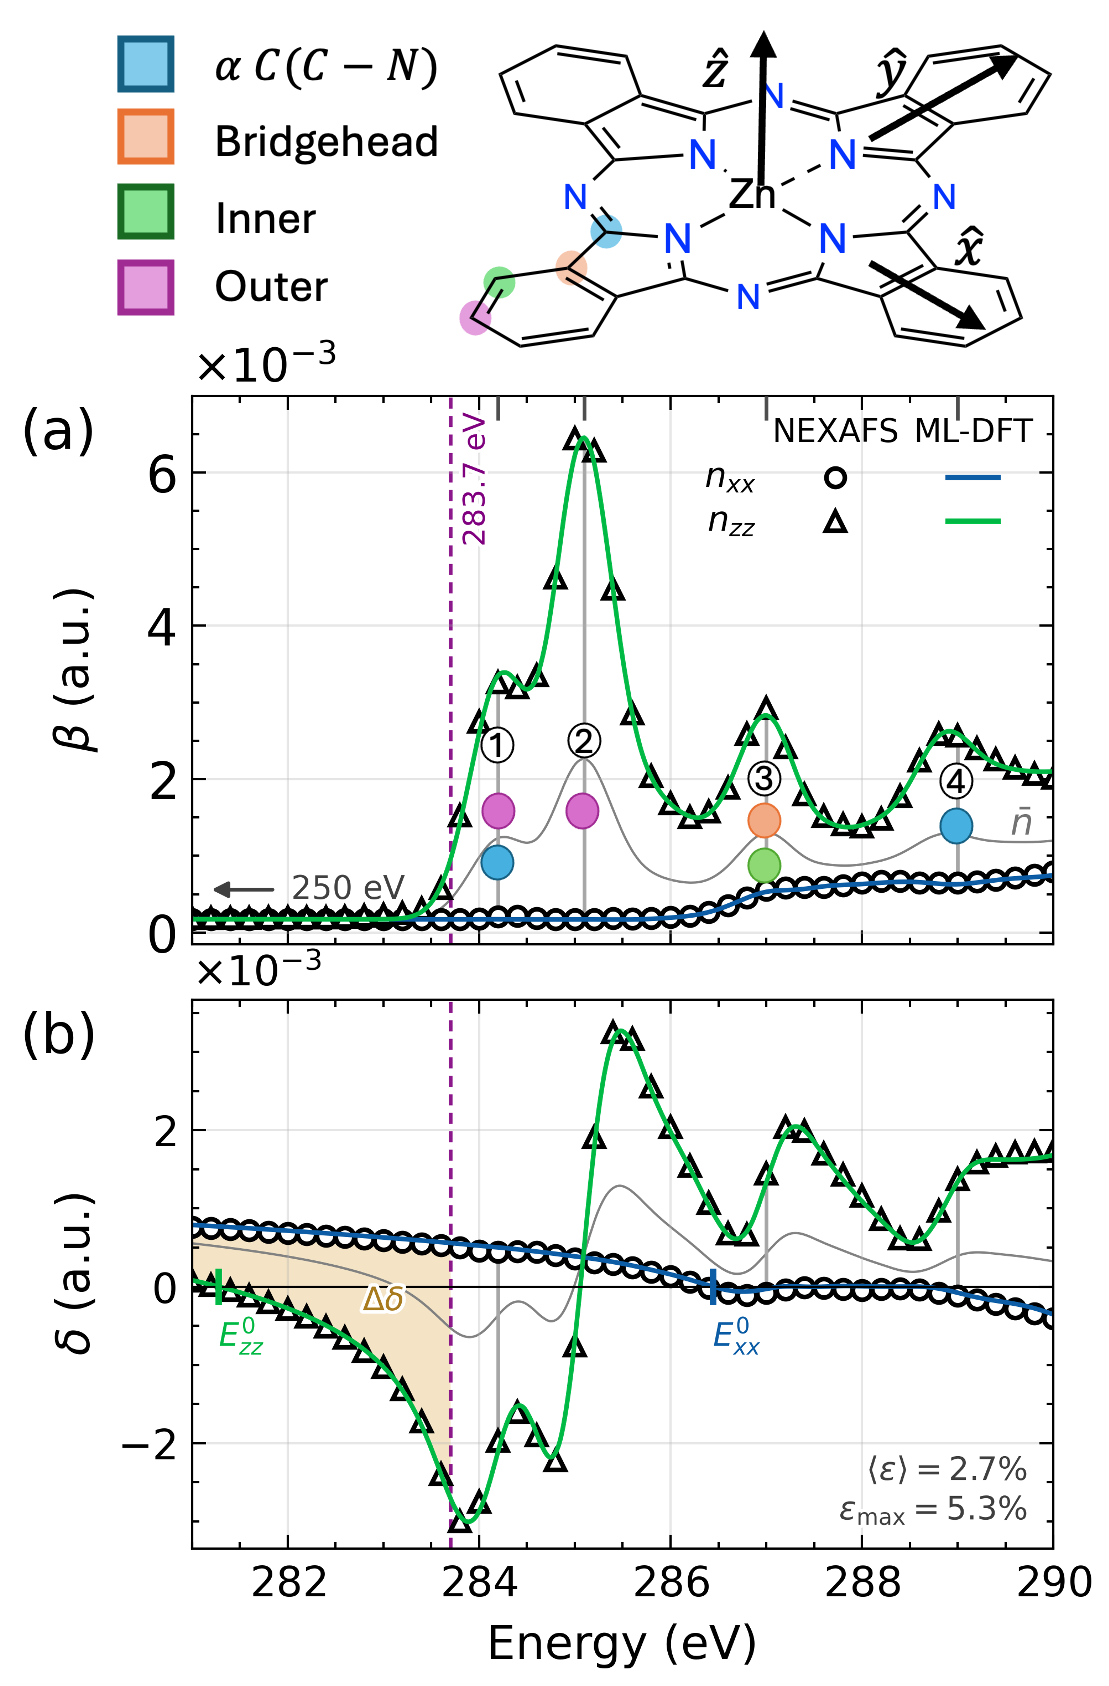
\includegraphics[width=0.45\linewidth,height=0.75\textheight,keepaspectratio]{fig4-01_ml-dft-tensor}
  \caption[An ML-DFT resonant optical model for ZnPc.]{An ML-DFT resonant optical model for ZnPc. ML-DFT (Traces) and angle resolved NEXAFS measurements (points), deviating by \(\epsilon = 2.7\%\) and \(\epsilon_{\max} = 5.3\%\) at resonance (1). Top, schematic of the molecular frame and the four inequivalent carbon excitation centers, colored as labeled. (a) \(\beta_{xx}\), \(\beta_{zz}\), and the isotropic average \(\beta\) (gray), numbered bars are fine structure resonances targeted for RSoXS measurement, with colored pips indicating the excitation centers dominating the transition. (b) \(\delta\) by Kramers-Kronig transformation,\autocite{kramers1927diffusion} with shaded \(\Delta\delta\) bounded by the zero crossings \(E^{0}_{xx}\) and \(E^{0}_{zz}\). Vertical purple dash is a diagnostic RSoXS energy.}
  \label{fig:4.1}
\end{figure}


\section{Constructing an ML-Refined DFT Optical Tensor}\label{sec:constructing-an-ml-refined-dft-optical-tensor}

We focus on thin films of Zinc phthalocyanine (ZnPc), a mature molecular platform spanning foundational studies of single-molecule photophysics and quantum optics\autocite{yang2020sub,zhang2016visualizing,luo2019electrically,cao2021energy,doppagne2018electrofluorochromism}, commercial photovoltaics\autocite{klenkler2015photovoltaic,pfeiffer2013organic}, thin-film transistors and sensors\autocite{boileau2019metal,comeau2022surface}, and photomedicines.\autocite{chornovolenko2025phthalocyanines,rak2023advances,luo2021nanoscale} Physical vapor deposition yields polycrystalline films with the molecular orientation commonly set by patterning underlayers. CuI and graphene pattern face-on orientation (molecules lying flat) with brickstone packing while Si patterns the edge-on orientation with herringbone packing\autocite{kato2020morphological,ngongangndjawa2015impact,schunemann2011zinc}. However, in situ coverage studies have suggested that ZnPc and other metal-Pc films might bear more complex microstructural states that evolve from the substrate to the vacuum interface.\autocite{derrien2022interfacial,yang2015molecular,yamamoto2022variation,deoteyza2006structural,osso2004structure}

On silicon, ZnPc assumes a monoclinic herringbone crystal structure\autocite{schunemann2011zinc,derrien2022interfacial} with a strong edge-on texture confirmed by ellipsometry and GIXRD (Supplemental Material, \suppsec{1}). AR-NEXAFS places the film-averaged macrocycle normal (\(\widehat{z}\) in \cref{fig:4.1} schematic) at a polar tilt of \(\gamma = \ang{74}\) from the substrate surface normal (Supplemental Material, \suppsec{1}, i.e. edge-on orientation). The molecular index of refraction tensor \(n_{ij}(E) = 1 - \delta_{ij}(E) + i\beta_{ij}(E)\) follows by projecting the experimentally measured \(\beta_{\theta}(E)\) (from AR-NEXAFS) onto the molecular optical axes (\cref{fig:4.1}a, symbols)\autocite{stohr2010nexafs,collins2012polarized}, using the molecule-to-film relation given in Supplemental Material, \suppsec{2}. Unfortunately, the measured optical anisotropy is a convolution of the transition dipole moments (TDM) and the film-averaged molecular tilt. Through our ML clustering algorithm we remove this ambiguity to extract the orientation of the principle TDMs calculated from DFT simulated NEXAFS.\autocite{murcia2026quantitative} TDM clusters are then refined to quantitatively reproduce AR-NEXAFS (Supplemental Material, \suppsec{3}) compared in \cref{fig:4.1}. The average error between the refined optical tensor in reproducing the AR-NEXAFS data is 2.7\% with all experimental features reproduced in \cref{fig:4.1}. Thus, the ML-DFT single molecule tensor fully captures the optical interactions emergent in the film, while assigning chemical character and TDMs to spectral features.

The first two TDM clusters orient along \(\widehat{z}\) and carry the dominant oscillator strength, producing a strong pre-edge birefringence (\(\Delta\delta\), \cref{fig:4.1}b) that eventually flips at higher energies. We exploit this in reflectivity measurements via two modes. First, with high-density sampling in energy up to just below the first absorption resonance, we locate the extinction of the s-polarized critical angle \(\theta_{c}^{s} = \sqrt{2\delta_{xx}}\) to inform the film averaged orientation at low radiation dose. Maximum q-range reflectivity is then collected at two book-ending diagnostic energies, maximizing sensitivity to thin buried layers. This pre-edge data reports the orientation of a generic conjugated framework rather than chemical identity. Chemical specificity is provided though RSoXS measurements at the fine structure resonances which resolve all four inequivalentcarbon environments of the macrocycle (labeled in \cref{fig:4.1} schematic and circles in \cref{fig:4.1}a) as determined through the DFT calculation.

\begin{figure}
  \centering
  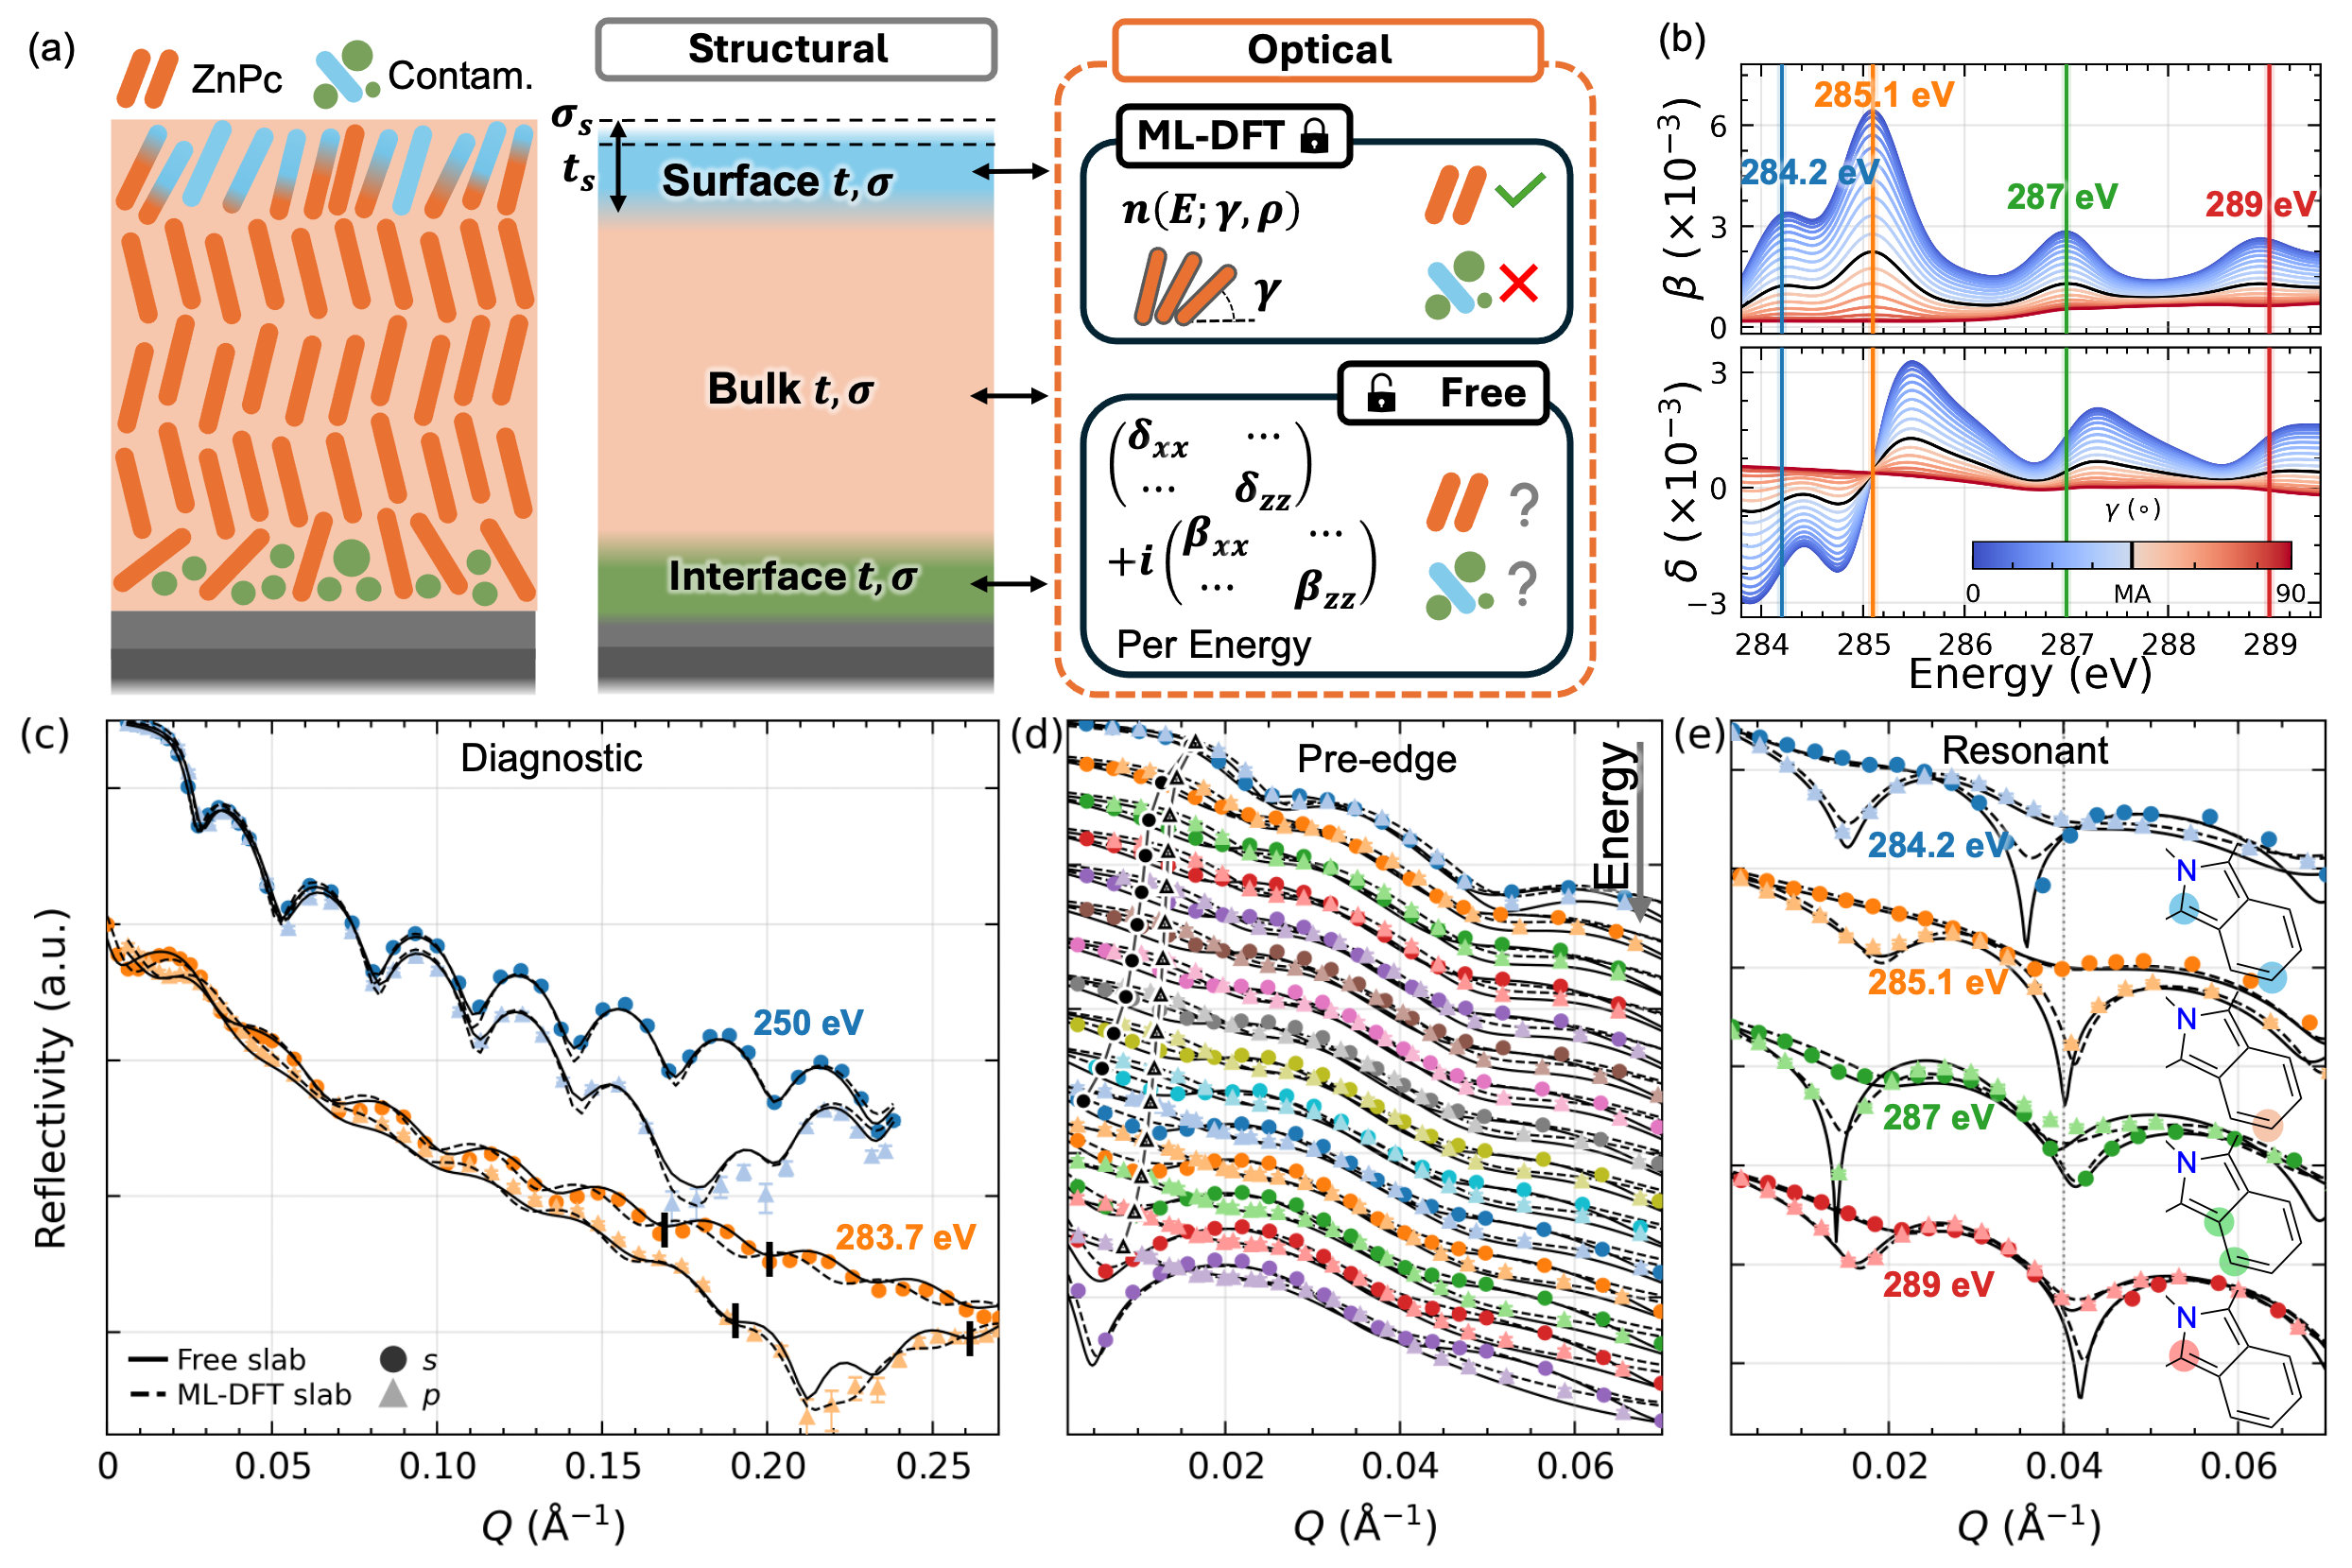
\includegraphics[width=\linewidth,height=0.75\textheight,keepaspectratio]{fig4-02_rsoxs-fits}
  \caption[Fitting energy and polarization-dependent RSoXS.]{Fitting energy and polarization-dependent RSoXS. (a) Reflectivity model description of the film using three ZnPc slabs on SiO\textsubscript{2}/Si with thickness \(t\) and roughness \(\sigma\) each, differing only by the optical parameterization of each slab with the Free model requiring four uniaxial components per energy per slab against the ML-DFT model with just two, molecular tilt \(\gamma\) and density \(\rho\) per slab. (b) Film out of plane tensor components built from \cref{fig:4.1} parameterized by tilt angle from face to edge on with the isotropic condition in black. Vertical lines denote the energies in the resonant series. (c-e) Reflectivity data (showing every fifth datapoint, Supplemental Material, \suppsec{5}), s-pol (filled circle) and p-pol (triangle, lighter), against the Free (solid) and ML-DFT (dashed) models for each energy domain: (b) diagnostic energies, (c) pre-edge, δ-crossing, (d) post-edge, (e) resonant. Ticks in (c) mark the Q-ranges of the largest divergences. Traced in (d) plots the critical angle for each s-and-p-pol across the pre-edge energies. Molecule frames inset in (e) highlight the carbon excitation centers within one outer ZnPc wing that dominate each TDM cluster.}
  \label{fig:4.2}
\end{figure}


\section{Direct, Quantitative Sensing of Molecular State with Depth}\label{sec:direct-quantitative-sensing-of-molecular-state-with-depth}

We analyze the reflectivity data across these energies via forward simulation where the film is modeled in a three-slab structure, each with a thickness \(t\) and roughness \(\sigma_{r}\), outlined in \cref{fig:4.2}a. Three slabs are required for a good fit and are presumed to capture unique chemical states and species at the surface, bulk and buried interface of the film. We then test two optical models to contrast the ML-DFT optical model with that of the traditional analysis. The traditional approach, designated the Free model, fits four uniaxial tensor components per energy per slab (\cref{fig:4.2}a). A secondary analysis must be developed to determine chemical nature, orientation, and density from these optical parameters. In contrast to this, the ML-DFT model uses the energy and polarization-dependent optical tensor from \cref{fig:4.1} (derived in Supplemental Material, \suppsec{4}, orientation dependence in \cref{fig:4.2}b) to directly parameterize density \(\rho\) and molecular tilt angle \(\gamma\) -- only two parameters total per slab and consistent across energy compared with 84 in the Free model. In this approach, different chemistries, such as oxidation or contamination in the surface, bulk or substrate layers will be manifest as fit variances at the molecule's key resonant energies (\cref{fig:4.2}e).

Fit quality between the two models differs by energy regime. Across the pre-edge and resonance series of \cref{fig:4.2}d and~e, the DFT model tracks the data with similar or better residuals than the free tensor model. The critical angles traced in \cref{fig:4.2}d, vertical black traces, highlight the underlying birefringence that is consistent with the ZnPc molecules oriented edge-on to the substrate. By contrast, the molecule's resonance series (\cref{fig:4.2}e) is sensitive to chemical and electronic orbital identity. Here the ML-DFT model fits better than the Free model (average deviation 1.7\(\sigma\) vs 2.2\(\sigma\), respectively). Since the ML-DFT model restricts only ZnPc to be present in the film, this result indicates a lack of measurable contamination or oxidation in the film to which interfacial layers are customarily assigned.\autocite{ferron2022characterization,mezger2011molecular,ferron2023composition,pasquali2014structural} Instead, these layers depict a unique molecular configurational state well described by the ML-DFT model.

\Cref{fig:4.2}c presents the largest divergences between the models, where the characteristics of the \qty{283.7}{eV} reflectivity profile are the most challenging to reproduce for the either model. At this energy, the ML-DFT model performs worse in the s-pol profile with a noticeable phase shift (ticks, \cref{fig:4.2}c) between the fringes in the data and model. Conversely, in the p-profile, the Free model fits worse and fails to capture the fringe structure around Brewster's angle (ticks, \cref{fig:4.2}c). Despite this, both models arrive at similar slab structures (\textbf{Tab.} \textbf{SI, SII}) that agree with total thicknesses from ellipsometry analysis (\suppfig{1}), yet the DFT model achieves this with more than \(10\times\) sharper parameter uncertainties than the Free model.

At this point, the Free model optical parameters must be analyzed further to interpret orientation and density. In contrast, these critical parameters are read directly from the ML-DFT model, quantitativelytracing the microstructure evolution through the film in three distinct densities and orientation states. The parameters of the central bulk layer agree well with tabulated density and orientation of herringbone ZnPc.\autocite{kato2020morphological,derrien2022interfacial} Separately, the surface and interfacial layers exhibit orientation and densities that do not agree with herringbone packing yet both carry the resonant anisotropy that only orientated ZnPc can produce -- in particular, the resonant amplitudes and even anisotropy flipping across the edge.

\begin{figure}
  \centering
  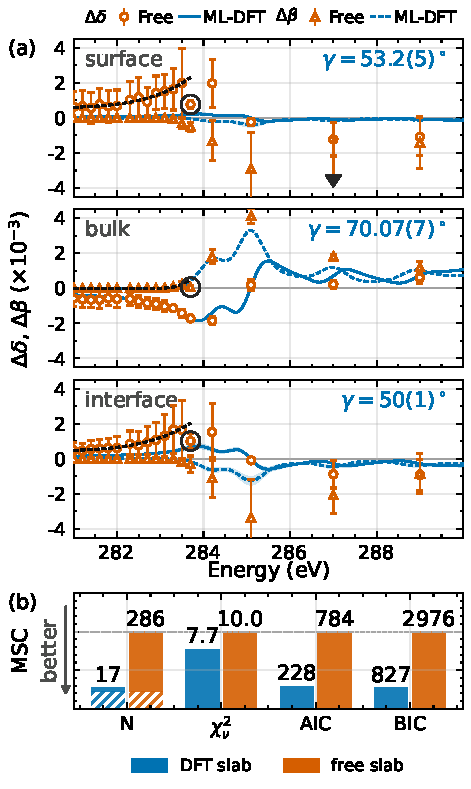
\includegraphics[width=0.45\linewidth,height=0.75\textheight,keepaspectratio]{fig4-03_model-comparison}
  \caption[Dominance of the ML-DFT model over traditional analyses.]{Dominance of the ML-DFT model over traditional analyses. (a) Birefringence \(\Delta\delta = \delta_{xx} - \delta_{zz}\) (circles, solid) and dichroism \(\Delta\beta = \beta_{xx} - \beta_{zz}\) (triangles, dashed) for the surface, bulk, and interfacial ZnPc layers. Orange points are Free tensor optical parameters fit independently per energy. Blue traces follow from the ML-DFT optical model with blue areas representing uncertainties. (b) Model selection criterion (MSC): reduced total parameter counts \(N\), \(\chi^{2}\), and the AIC and BIC criteria for the two models where lower values indicate the preferred model. Hashed regions in \(N\) represent constrained experimental offset parameters (Supplemental Material, \suppsec{5})}
  \label{fig:4.3}
\end{figure}


The optical properties of the two models, as shown in \cref{fig:4.3}a (expanded in \suppfig{10}), agree closely within the bulk, while those of the Free model surface and buried interface layers are both more extreme and highly uncertain, enough such that there are no significant disagreements between the models. The comparison of the models highlights several issues with the Free model. For instance, the unphysical dichroism at \qty{287}{eV} (black arrow pointing off scale in \cref{fig:4.3}a) highlights the fact that there are no constraints against unphysical results. In particular, there is no known way to assure the Free model optical parameters obey Kramers-Kronig consistency without excessive energy sampling.\autocite{ferron2023composition,stone2012kramers} The second notable issue is interpreting the Free model optical parameters for orientational or chemical state. In particular, the low energy trends in \cref{fig:4.3}a are discontinuous at the diagnostic dataset at \qty{283.7}{eV} (circled points in \cref{fig:4.3}a), resulting in contradicting conclusions of the molecular orientation state depending on which energy is analyzed.

Not only is the ML-DFT model superior, being physically constrained and interpretable, but all statistical metrics demonstrate its advantages (\cref{fig:4.3}b) due especially to the reduced total number of parameters in the model (\emph{N}). The reduced chi square parameter \(\chi_{\nu}^{2}\) suggests that the DFT model reaches the best agreement with the experiment across the full set of energies. The Bayesian and Akaike information criterion (BIC \& AIC) measure the weight of evidence for each model and the expected performance for new measurements, respectively. From these results, we conclude that the DFT model achieves a drastic statistical improvement in fit quality with \(17\times\) fewer parameters and \(10\times\) smaller parameter uncertainties, while presenting directly interpretable results that are useful to interrogate the molecular state.

\begin{figure}
  \centering
  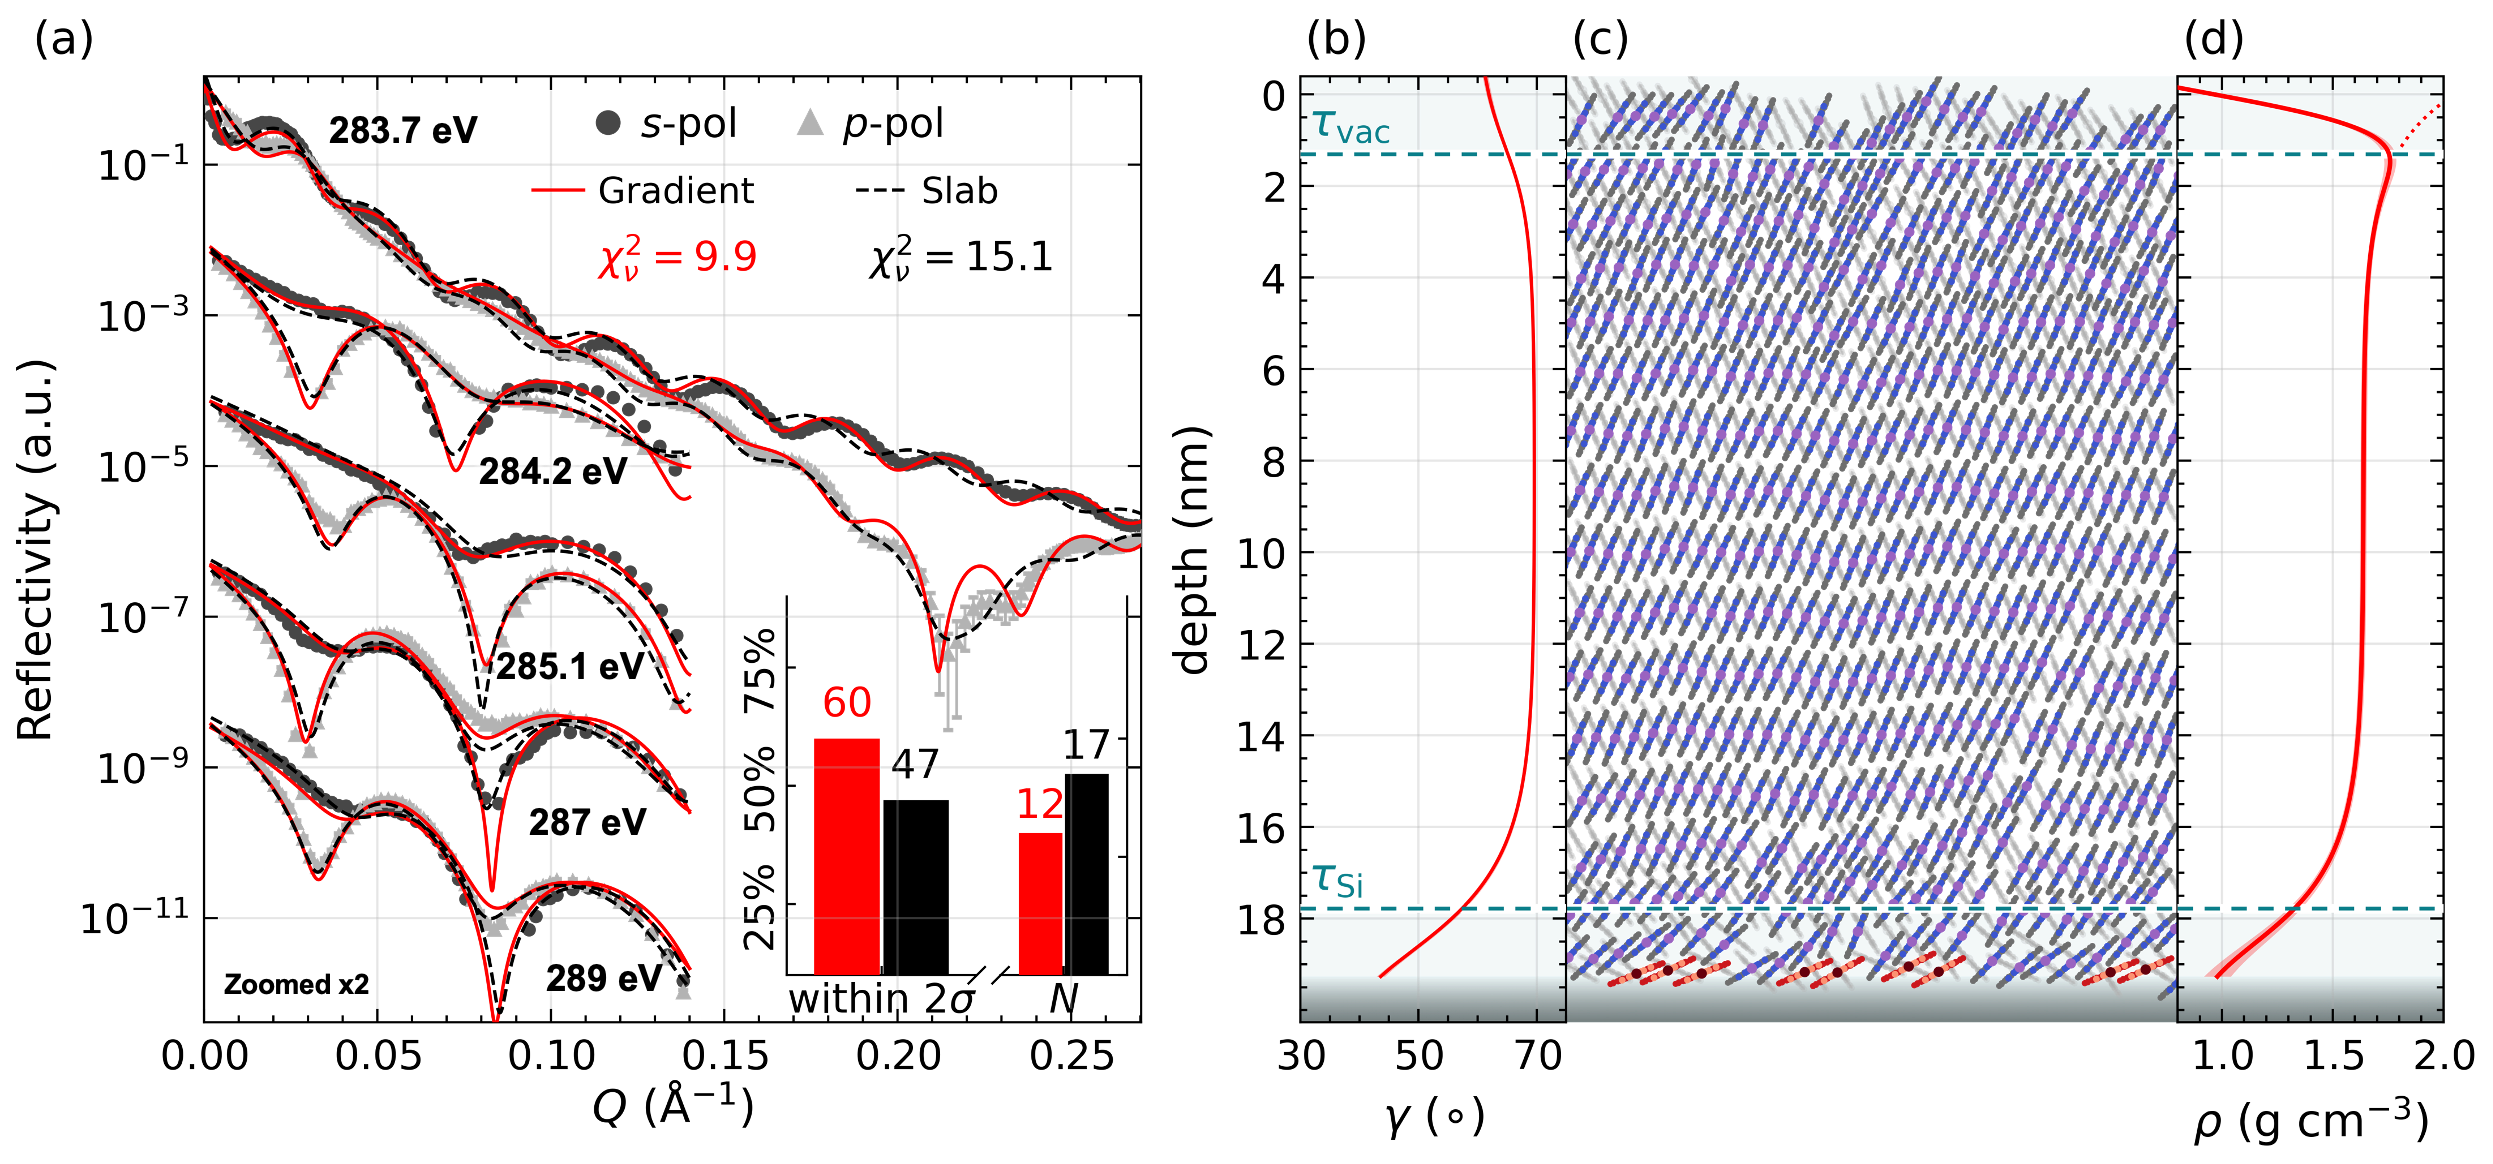
\includegraphics[width=\linewidth,height=0.75\textheight,keepaspectratio]{fig4-04_depth-profile}
  \caption[Revealing sub-monolayer orientation and density gradients at a buried interface.]{Revealing sub-monolayer orientation and density gradients at a buried interface. (a) s- and p-pol reflectivity fits to \qty{283.7}{eV} and resonant energies for the slab model (dashed), against the orientation gradient (red). For clarity, the q-range is stretched by \(2\times\) for the resonant profiles. Inset reports model fit quality as \(2\sigma\). (b-d) Real space analysis of molecular state versus depth. (b) orientation and (d) density depth profile of the gradient model with characteristic interfacial widths \(\tau_{\mathrm{Si}}\) and \(\tau_{\mathrm{vac}}\) and RMS surface roughness, shaded bands representing 95\% confidence (2σ). (c) Visual reconstruction of the molecular state with depth consistent with orientation, density, and diffraction measurements. Gray molecules represent a layer behind the colored molecular layer in the front.}
  \label{fig:4.4}
\end{figure}


\section{Sub-monolayer Interfacial Physics}\label{sec:sub-monolayer-interfacial-physics}

Without needing to account for unique chemical species at the boundaries of the ZnPc bulk layer, the independent slab model is no longer physically motivated. Instead, we develop a single slab gradient model based on the physics of a continuous second order transition from a pinned molecular state due to surface energies that evolve toward an energy-minimized state in the bulk (derivation in \cref{sec:orientation-gradient-theoretical-foundation}). This results in a description physically matched to an evolving growth front during deposition with each deposited layer taking its orientation from those beneath it. This gradient model resolves orientation as a smooth function of depth, parameterized by the bulk state and two exponentials that transition over characteristic lengths \(\tau\) toward the pinned state at each interface. Besides incorporating the physics at play during deposition, this structural model also has fewer parameters than the slab model.

The fit using the graded interface model (with ML-DFT modeling optics) is compared to the slab model in \cref{fig:4.4}a for the diagnostic profile at \qty{283.7}{eV}, together with the resonant series but neglecting the rest of the data. Notably, the erroneous phase shift of the fringes in the slab model is removed in the gradient model and the Brewster angle is reproduced significantly better than the slab model. These fit improvements along with the reduced number of parameters enable the best goodness of fit, indicating this model recovers the true orientation and density gradient within the sample more accurately than what the traditional slab picture can achieve.

\begin{table}
  \centering
  \caption{Best fit parameters from the orientation and density gradient model. Total film thickness is \(\qty{192.7(4)}{\angstrom}\) with RMS surface roughness of \(\qty{6.8(4)}{\angstrom}\). Errors are reported as \(2\sigma\) from the covariance matrix.}\label{tab:4.1}
  \begin{tabular}{l S[table-format=2.1(1)] S[table-format=1.2(1)] S[table-format=2.1(1)]}
    \toprule
    Region & {\(\gamma\) (\unit{\degree})} & {\(\rho\) (\unit{g.cm^{-3}})} & {\(\tau\) (\unit{\angstrom})} \\
    \midrule
    Surface & 58.7(6) & 2.0(1) & 13(1) \\
    Bulk & 69.6(2) & 1.64(1) & {---} \\
    Interface & 38(1) & 0.87(7) & 14.9(1) \\
    \bottomrule
  \end{tabular}
\end{table}

The recovered structure is plotted in \cref{fig:4.4}b and~d with fit parameters in \cref{tab:4.1}. The bulk tilt is consistent with the film averaged orientation from AR-NEXAFS (\suppfig{5}). At the buried interface, the profile descends to a lower density, face-on orientation, while at the free surface the orientation relaxes to a lower angle and a slightly higher density than bulk. This profile is consistent with a second film grown under identical conditions with a different total thickness (\suppfig{10}). The comparison and consistency between independent films, suggests these parameters may be intrinsic to the growth conditions of the ZnPc system and dictated directly by the free energy potentials at the vacuum and silica interfaces.

\Cref{fig:4.4}c presents a molecular level, real space reconstruction of the film through data fusion of our RSoXS analysis, XRD lattice spacings (Figs.~S11 and~S12), and a force-field model of the molecule. Notably, the entire film is only \({\sim}\)15 monolayers thick with the substrate surface energy affecting a region equivalent to a single monolayer. However, the fact that the graded interface model fits better than the discrete slab model reveals that the continuous density and orientation variation over that region represents a real structural variation resolved by this analysis. In fact, the unique tilt in the last few angstroms at the interface, can only manifest with sub-monolayer coverage of ZnPc molecules that are pinned relatively flat on the substrate. This confined feature is well below the experimental diffraction limit (\(2\pi/q_{\max} > \qty{23}{\angstrom}\)). However, scattering from such features still modify the amplitude and phase of the measured fringes. A Fisher sensitivity analysis (\suppfig{13}) determines that these sub-monolayer features are uniquely captured and constrained by our ML-DFT optical model which locks these effects as a function of energy and polarization to enable recovery of the molecular state below the diffraction limit.

\section{Surface versus Bulk Dynamics in Film Growth}\label{sec:surface-vs-bulk-dynamics-in-film-growth}

These results are direct evidence against the model of substrate patterning of bulk molecular orientation and provide evidence toward an alternative model that incorporates intermolecular interactions at the growth front. One explanation for our results is that the orientation a planar molecule adopts during deposition reflects a competition between the substrate adhesion, which favors face-on alignment and intermolecular \(\pi - \pi\) cohesion, which favors edge-on packing. The gradient then traces the crossover from a low dimensional interfacial coupling to the three-dimensional growth mechanism that sets the bulk texture. The lower density and face-on alignment at the interface indicates that the packing state here is not the relaxed herringbone but possibly a primordial face-on brickstone packing structure which typically exhibits such properties.\autocite{derrien2022interfacial} We expect that evaluating these effects on interfacial states in molecular systems will enable control of emergent phenomena at these interfaces, for example, charge generation and recombination in organic solar cells and OLED technologies\autocite{tumbleston2014influence,yokoyama2011molecular} or charge and ion transport in transistors\autocite{pei2020semiconductor} or electrochemical devices.\autocite{khan2025local,flagg2023resonant,mayer2026lumen,trigg2018self,dong2010super} The same sub-monolayer sensitivity extends directly to self-assembled monolayers, where incomplete or defective coverage during assembly is now recognized as the limiting factor for both efficiency and thermal stability in state-of-the-art perovskite solar cell devices.\autocite{jiang2025toughened} More broadly the analysis can be applied to any interface, polymer, alloy, or few-layer system whose function depends on a coverage-dependent structure that a bulk-averaged measurement cannot resolve.

The surface densification measured here, along with an orientation approaching the magic angle also indicates a distinct state from the bulk, where the higher density and disorder may be caused by the physics of surface tension during deposition. In this case, these boundary layers are not the adventitious hydrocarbon contamination nor oxidation to which film-averaged analyses and other RSoXS studies customarily assign them\autocite{ferron2023composition,fostiropoulos2019temperature} but rather potentially a disordered state before the ZnPc molecules fully crystalize. Moreover, this demonstrates that in studies characterizing structure of films deposited with varying coverages\autocite{derrien2022interfacial,yamamoto2022variation,deoteyza2006structural} do not measure the state expected in a continuously deposited film, since both substrate and free surface energetics pull the state away from the final buried states.

The new RSoXS analysis provides a depth sensitivity to buried molecular state applied in a broad range of physical conditions, allowing quantitative studies of interfacial phenomena like crystal growth, kinetic deposition, and solvent interaction. The same construction extends to molecules with additional orientational and chemical freedom, to polymers, alloys, and mixed oxidation states or orbital hybridization affecting unoccupied molecular orbitals. The analysis is, furthermore, applicable to scattering geometries beyond reflectivity, enabling local chemical, electronic, and physical analyses of inaccessible buried interfaces that govern function across material systems and nanostructures. Connecting scattering features that vary with energy and polarization, our ML-DFT optical model can not only provide these states directly but also push the resolution well beyond the traditional diffraction limit.

In summary, we introduce a resonant X-ray scattering analysis that directly interprets the quantitative physicochemical molecular state in a buried nanostructure based on an ML-refined DFT optical model. The analysis substantially improves parameter precision and resolves structure finer than the diffraction limit, so that the molecular state at an interface can be characterized directly. Applying this analysis to ZnPc films, we find that hypotheses of chemical contamination at the film surface and buried interface are rejected in favor of the molecules exhibiting a novel packing and orientational state. Introducing a structural model based on the dynamics of film growth, we reveal evidence to reject hypotheses of substrate patterning of the bulk packing state in favor of a competition between two- and three-dimensional growth that determines the interfacial evolution of the molecular states. This statistical analysis of the final buried molecular state contrasts with checkpoint studies that track a growth front that is likely only in a temporary state. We expect this non-destructive view inside buried interfaces to enable deliberate control of the interfacial states that govern function in organic devices.

\section{Methods}\label{sec:methods}

\textbf{Film growth:} Small molecule ZnPc (C32H16N8Zn sourced from Sigma Aldrich) with purity \(\geq 99.5\%\) was further purified in the physical vapor deposition (PVD) chamber (base pressure \(< 1 \times 10^{- 7}\) Torr) by gradually heating, approaching ZnPc sublimation temperature over approximately an hour until no further off gassing of contaminants were detected by the quartz crystal monitor (QCM). Thin films (\({\sim}\)\qty{20}{nm} measured by QCM) of ZnPc were deposited at \(.2\ \mathring{\mathrm{A}}/s\) on high conductivity polished Si wafers (University Wafers). Wafers were cleaved \qty{1}{cm} x \qty{3}{cm} and cleaned via sonication in deionized water, acetone and isopropyl alcohols before a 30 min UV ozone bake. ZnPc was either deposited directly onto these wafers to create the herringbone crystal structure, or onto a thin Copper Iodide (CuI, \qty{3}{nm}) patterning layer producing a face on brick-stone polymorph. Substrate temperature was either set to the ambient room temperature (24 C), by liquid nitrogen cooling (-50 C), or by thermal substrate heating (100 C). For brick-stone samples, CuI and ZnPc depositions were performed sequentially under the same vacuum, with 20 min between depositions to return to the base pressure. Films for RSoXS were stored under an inert N2 atmosphere and transported to the ALS under vacuum. Auxiliary pre characterization measurements were performed on separate films from the same batch to avoid surface contamination and oxidation prior to RSoXS.

\textbf{VASE:} Variable angle spectroscopic ellipsometry (VASE) (\suppfig{1}) was performed using a J.A. Woollam alpha-SE to pre characterize layer thickness and molecular orientation. Data was collected at three incidences (\ang{65}, \ang{70}, and \ang{75}) targeting a sample from the same PVD batch and measured using vendor supplied CompleteEase software. Optical constants where modeled using a B-spline producing similar spectra to literature.\autocite{kozlik2013optical} The results and analysis of VASE data are discussed in Supplemental Material, \suppsec{1}

\textbf{GIXRD:} Grazing incidence wide angle x-ray diffraction (GIXRD) measurements (\suppfig{2}) were performed at Washington State University on a Xenocs Xeuss 3.0 with a focused Cu X-ray source (\(\lambda = \qty{1.5418}{\angstrom}\)), under vacuum at \qty{72}{mm} sample-detector distance with incident angle set to \(\ang{0.2}\). The sample-to-detector distance and beam center were calibrated with a silver-behenate standard. 1D reduction of GIWAXS images was done using NIKA software\autocite{ilavsky2012textless} and peak positions were obtained by fitting Gaussian line shapes to the reduced profiles. The lamellar reflection lies along the \(q_{z}\) and the \(\pi - \pi\) reflection is in plane corresponding with the edge on texture of the \(\alpha\) herringbone polymorph reported for vacuum deposited ZnPc and CuPc.\autocite{hoshino2003redetermination} The results and analysis of GIXRD data are discussed in Supplemental Material, \suppsec{1}.

\textbf{AFM:} Atomic force microscopy (AFM) height maps were acquired on a Bruker Dimension Icon in tapping mode with a TESPA-V2 SAMPLE probe. Scans where processed using Gwyddion\autocite{necas2012gwyddion} to extract root-mean-square (RMS) roughness values. Film morphologies and RMS roughness values were used to pre-characterize film surface roughness and morphology RSoXS measurements. The surface topology is included in \suppfig{4} and the discussion in Supplemental Material, \suppsec{1} and \textbf{1.4}.

\textbf{NEXAFS spectroscopy:} NEXAFS spectra were collected at the Soft X-ray Spectroscopy (SXR) beamline of the Australian Synchrotron, part of ANSTO in total electron yield mode on Si wafers.\autocite{heilman2026x} Samples where grown under the same conditions Spectra were collected at five sample alignments with respect to the incident electric field polarization vector with respect to the surface normal (\(\ang{20},\ \ang{40},\ \ang{55},\ \ang{70},\ \&\ \ang{90}\)). NEXAFS was collected over the energy range of 270-\qty{350}{eV} and normalized to the energy dependent intensity fluctuation and optical loss via a direct photodiode measurement, and Au mesh drain current. Mass absorption was computed via normalization in the pre and post edge regions to the bare atom mass absorption of ZnPc as extracted from the CXRO Henke atomic scattering factors.\autocite{henke1993x}

Molecular tilt angle was extracted via the DFT cluster and refinement process. As the final step of the refinement process, the molecular polar tilt angle \(\gamma\) is fit using the TDM cluster orientations prescribed by DFT providing a measure of the molecular orientation (\suppfig{5}). This fit produces a reduces \(\chi^{2}\) goodness of fit statistic of .213 indicating very good agreement between the model and experimental data. The molecular tilt angle of \(\ang{74}\) agrees with all other characterizations of the ZnPc edge-on herringbone polymorph described in this study and is taken as the coarse-grained molecular orientation within the films measured under RSoXS (full analysis in Supplemental Material, \suppsec{3}).

\textbf{Density Functional Theory:} A time independent transition potential calculation using the StoBe library was performed on a single molecule of ZnPc. A HCH approach sets the manifold of transition energies, along with each TDM and oscillator strength, while the \(\Delta KS\ \)method is used to fix the absolute energy associated with each transition. For details see our previous work.\autocite{murcia2026quantitative} The molecular geometry was extracted from a crystallographic structure file (.cif)\autocite{mai2020data} as it produced results with a higher initial agreement to experiment compared to thermodynamically relaxed structures, or those relaxed from molecular force fields. The final calculation results are provided in Supplemental Material, \suppsec{1}.

\textbf{ML-clustering and refinement:} The ML optimized optical tensor is constructed through hierarchical agglomerative clustering to extract principal TDM clusters. Exact implementation details may be found on GitHub or through our previous work.\autocite{murcia2026quantitative,victormurcia2025wsu} TDM clusters are sequentially refined to quantitative agreement with experimental AR-NEXAFS by fitting oscillator strength, excitation energy, and TDM orientation. Optimal hyperparameters, oscillator strength threshold and overlap percentage were investigated by evaluating this best fit metric on an even grid \(OS \in \lbrack 0,\ 10\rbrack\ \&\ OVP \in \lbrack 25,75\rbrack\) with details in Supplemental Material, \suppsec{3} and highlighted in \suppfig{7}. From the family of hyperparameters that perform well on this metric, the refinement performance is additionally weighted by the adherence to the original DFT spectra and TDM cluster families such that the refinement step does not significantly alter the DFT calculation. Here we chose the best clustering parameters of \(OS = 0.25\) and \(OVP = 52.5\) with the full evaluation matrix in \suppfig{7}. In general, we find good clustering and convergence for all \(OVP \in \lbrack 50,55\rbrack\), with significantly worse performance outside of these bounds. Moreover, we find that \(OS \in \lbrack.1,8\rbrack\) performed similarly, yet parameter agreement with originating DFT degrades rapid for larger \(OS\), while the refinement never converse for \(OS < .1\).

\textbf{RSoXS collection:} Polarized resonant soft x-ray reflectivity was measured at beamline 11.0.1.2 of the Advanced Light Source, Lawrence Berkeley National Laboratory, following the procedure established by Ferron et al.\autocite{ferron2023composition} Samples are transferred from inert storage to the end station where specular reflectance is captured on the CCD area detector with thermals managed by thermos-electric cooling. The sample surface is aligned to the goniometer axis of rotation by an iterative process that refines the sample rotation and height. Incident flux was attenuated using the scatter slits together with the higher order suppressor to avoid detector damage. Because the total reflectance varies by more than the detectors dynamic range, reflectivity is captured in overlapping \(\mathbf{q}\) subsets with suppressor settings and exposure time raised at each boundary once reflectivity reaches the noise floor.

Data is collected first in s polarization and then in p polarization beginning at \qty{250}{eV}, below the carbon K edge, and stepping upward through the resonance, for 21 photon energies collected in batches of five energies with the axis of rotation alignment was reevaluated between energy batches. Upon polarization change, optics were allowed to re equilibrate to the new heat load for 30 min before alignment was recalibrated. The complete dataset was acquired within a single 12 h shift. Photon energy was calibrated against the transmission NEXAFS of a polystyrene standard at the beginning and at the end of the shift with no discernable shift, bounding the energy drift over the experiment to the width of the primary polystyrene feature.

\textbf{RSoXS reduction:} Reflectance was reduced from the two-dimensional detector images using the RSoXS-reduce package.\autocite{alsrsoxspxrreduce2026als} The specular spot was located on each frame and its intensity integrated over a fixed region of interest. An equal region displaced along the same detector row provided the background, so that subtraction removes the systematic row-wise readout offset in addition to dark current and stray light. Reflectance was then formed by dividing the background-corrected specular intensity by the incident \(I_{0}\) recorded at the start of each reflectivity profile through the averaging of five direct beam measurements.

At each energy, full multi-decade reflectivity profiles are constructed by properly scaling and joining the overlapping \(\mathbf{q}\)-subsets measured at different attenuation and exposure time. An effective \(I_{0}\) is computed from the four overlapping points, and the subsets were joined to form a singular continuous reflectivity profile for each measured energy. Reported uncertainties combine per-pixel effective \(I_{0}\) with a \(\mathbf{q}\)-dependent envelope accounting for the increasing ambiguity between specular and diffuse reflectivity at higher \(\mathbf{q}\) using the following equation:

\begin{equation}
  \sigma(E,\mathbf{q}) = a R_{\mathrm{exp}}(E,\mathbf{q}) + b\,\mathbf{q}.
  \label{eq:uncertainty-envelope}
\end{equation}

With \(a = .08\) and \(b = .5 \times 10^{- 6}\), which is a feasible approximation for experimental error under these considerations (discussion in Supplemental Material, \suppsec{5}).

\textbf{RSoXS structural and optical modeling:} Reflectivity is computed from the 4x4 transfer matrix using the \pkg{refloxide} package.\autocite{alsrsoxsrefloxide2026als} The film was modeled as three ZnPc slabs, denoted surface, bulk and interface, on a native SiO\textsubscript{2} layer and a semi-infinite Si substrate. Thickness and roughness of each ZnPc slab together with the oxide thickness and roughness give eight structural parameters. Reflection and transmission coefficients were computed at each photon energy and scattering vector with the 4x4 transfer matrix formalism matching boundary conditions at the five interfaces, with interfacial roughness entering in the Nevot-Croce sense as an exponential attenuation representing off-specular diffuse scattering from a faceted interface.\autocite{nevot1980caracterisation} Vacuum, silicon dioxide, and silicon were assigned to tabulated bare atom optical constants,\autocite{henke1993x} with an energy-independent density allowed to vary within (2, 2.8) g cm\textsuperscript{-3} to accommodate stochiometric deviation from the tabulated values. The forward model was evaluated using \pkg{refloxide}, and the objective and parameter machinery where provided by \pkg{refnx}.\autocite{nelson2019textless}

Two optical parameterizations were compared on this identical structure. The free tensor parameterization assigns each ZnPc slab an independent birefringence, dichroism, isotropic \(\beta\) and isotropic \(\delta\) at every measured energy, constraining to ranges dictated by the starting optical model, amounting to 252 optical tensor components. The DFT parameterization instead describes each slab energy-independently by a molecular orientation and a density, with one energy offset term common to all layers absorbing the calibrated difference between the NEXAFS and RSoXS instruments, amounting to seven parameters for all three slabs. A detailed parameter accounting and comparison with prior art is discussed in Supplemental Material, \suppsec{5}.

Experimental corrections were applied per energy and per polarization as a normalization scale factor and an angle-of-incidence offset, following Ferron et al.,\autocite{ferron2023composition} adding four terms per energy at 84 in total. The refinement therefore varies 101 parameters for the DFT model and 350 for the free tensor model. Bound on the correction terms, and the correlations they induce are described in Supplemental Material, \suppsec{5}.

All energies and polarizations are co-refined against a single global objective, so that the structural parameters are shared across the dataset and only the optical and correction terms carry energy indices. The log-likelihood assumed Gaussian errors at the uncertainties propagated though reduction, and all varying parameters were assigned uniform priors over their stated bounds. The maximum likelihood parameter set was located by differential evolution over the full bounded space, in parallel with deferred population updating and a local polish step using the L-BFGS-B algorithm, avoiding dependency on initial conditions. Reported parameter uncertainties are then taken from the inversion of the Hessian evaluated in the final polish step. Model comparison uses reduced chi square together with the Akaike and Bayesian information criteria.

\textbf{Unit cell construction:} Unit cells used for molecular dynamics simulations are constructed though fusion of GIXRD \(d\)-spacings with literature unit cells. The rigid ZnPc molecule originates from the same \(\beta\)-ZnPc (\suppfig{12}a) crystallographic results used for DFT simulations.\autocite{mai2020data} Lennard-Jones parameters are GAFF2, with UFF for the Zn coordination center. Charges are fitted using the B3LYP/def2-SVP electrostatic potentials and used to set the electrostatic repulsion between molecules.

The \(\beta\)-ZnPc stable polymorph with a known structure serves only as the validation target. A suitable unit cell was constructed from the chemically similar \(\alpha\)-CuPc by placing rigid ZnPc molecules within the CuPc unit cell. Lattice parameters \textbf{a} and \textbf{c} are set by the lamellar spacing (002), with \textbf{b} set by the \(\pi - \pi\) packing. The molecular tilt angle is scanned and compared to the GIXRD patterns though a fiber-texture forward model, with other unit cell angles set by minimizing the lattice energy (UFF+ESP). The resulting lattice parameters are tabulated in \supptab{3} with the resulting crystallographic (.cif) structure available and visualized in \suppfig{12}b. The final unit cell is then thermally relaxed by rigid-body NPT at \qty{300}{K}, with independent barostats on each axis such that the force fields set the lattice and herringbone arrangements. Over this range the minimum enthalpy cell produces a tilt of \(\ang{72(1)}\) and a density of \(1.657\) g/cm\textsuperscript{3} against \(\ang{69.6(2)}\) and \(1.64(1)\) g/cm\textsuperscript{3} from RSoXS and reproduces the lamellar and (002) spacings within 1.5\%. The final relaxed unit cell is visualized in \suppfig{12}c used in the remaining MD simulations.

\textbf{Real space molecular visualization:} Molecular packing in \cref{fig:4.4}c is a molecular dynamics (MD) reconstruction of the film. It is built from the fitted depth profiles of \cref{fig:4.4}a and~b and relaxed in LAMMPS.\autocite{thompson2022lammps} ZnPc is treated as a rigid body in the molecular frame used for the DFT calculations. Lennard-Jones parameters are taken from GAFF2, with UFF for Zn, and atomic charges are fitted to the B3LYP/def2-SVP electrostatic potential. This force field reproduces the \(\beta\)-ZnPc unit cell at \qty{100}{K} to within 1.5\% on each axis (SI).

The film is constructed for pure visualization by data fusion with the fitted depth profiles, GIXRD, and the fitted electrostatic potentials. The molecular frame is the same used for the DFT calculations (C32H16N8Zn, \(M = 577.9\) g/mol). It's van der Waals envelope gives an in-plane diameter of 14.5 \(\mathring{\mathrm{A}}\) and a face-to-face thickness of \(\qty{3.6}{\angstrom}\), and the \(\pi\)-stacking separation is taken as \(\qty{3.4}{\angstrom}\). At each depth \(z\ \)the molecular tilt is \(\gamma(z)\) from the orientation profile, and the area per molecule in the drawing plane is \(M/(\rho(z)N_{A}t)\), with \(\rho(z)\) the fitted density profile and \(t = \qty{14.4}{\angstrom}\) the extrusion thickness of the slab that the projection represents. The packing density of the molecules in the illustration is therefore self-consistent with the density and orientation gradients from \cref{fig:4.4}b and~d. The projected cell is orthogonal, carrying a lamellar period along \(z\) and a column period in plane whose ratio is fixed by the molecular diameter, the \(\pi\) stacking separation and \(\sin^{2}\left( \gamma(z) \right)\). The lamellae period is modified by the interdigitation between neighboring lamellae, set by a dimensionless factor \(f = 0.96\), so adjacent layers can overlap by \(4\%\) of the molecular diameter. This together with the herringbone splay and positional and orientational disorder are set only for visual continuity and are neither empirical nor derived factors.

The depth dependent lamellae and \(\pi\) d-spacings are compared with diffraction orders derived from experimental GIWAXS measurements in \suppfig{11}. Because both the cell area and its aspect ratio vary with depth, each z monolayer contributed its own pair of spacings rather than a single value, so the predicted diffraction positions are a taken as the maxima of these depth distributions, weighted by the local density and the Debye-Waller factor built from the drawn positional disorder. The lamellar and \(\pi\) spacing periods agree with the measured peak centers to around \(2\%\), treated as a secondary consistency check of the molecular visualization.

\textbf{Data Availability:} NEXAFS data that support the findings of this study have been deposited in X-ray Atlas (\url{https://xrayatlas.wsu.edu}) with the accession code \href{http://xrayatlas.wsu.edu/d/193bc0c5}{193bc0c5} and are archived at Zenodo (\url{https://doi.org/10.5281/zenodo.22742990}).\autocite{heilman2026x} RSoXS reflectivity curves, GIWAXS, non-resonant XRR, VASE, and AFM topography together with the fitted model parameters that support the findings of this study are available from the corresponding author upon reasonable request.

\textbf{Code availability:} The source code used for reflectivity analysis may be found on GitHub (\url{https://github.com/wsu-carbon-lab/refl-analysis}).\autocite{heilman2026refl} The code for the RSoXS 1D to 2D data reduction can be found on GitHub (\url{https://github.com/als-rsoxs/pxr-reduce}).\autocite{alsrsoxspxrreduce2026als} The source code used to compute reflectivity and fit RSoXS data may be found on GitHub (\url{https://github.com/als-rsoxs/refloxide}).\autocite{alsrsoxsrefloxide2026als} The source code used for the DFT clustering and optical model generation may be found on GitHub (\url{https://github.com/wsu-carbon-lab/dft-learn}).\autocite{victormurcia2025wsu}

\textbf{Acknowledgements:} This research used resources of the Advanced Light Source, which is a DOE Office of Science User Facility under contract no. DE-AC02-05CH11231. Part of this work was carried out on the Soft X-ray Spectroscopy (SXR) beamline of the Australian Synchrotron, part of ANSTO. The authors also acknowledge the National Energy Research Scientific Computing Center (NERSC) provide supercomputer resources to this work for the DFT calculations, and RSoXS fits. The authors also acknowledge Dr. Thomas Ferron, Dr. Cheng Wang, and Dr. Kas Andrle form the Advanced Light Source of Lawrence Berkeley National Laboratory for their training and guidance in data collection, reduction, and fitting analysis. The authors also thank Dr. Arda Gozen from the School of Mechanical and Materials Engineering of Washington State University for AFM support on measuring soft nanoscale films. Fable 5 from Anthropic was used for minor copy editing and code generation under the ALS computing group's team plan. The authors also thank Dr. Daniel Dougherty from North Carolina State University and Dr. Dean DeLongchamp from the National Institute of Standards and Technology for their reading and consultation of the manuscript.

\chapter{Tracking the Evolution of Individual Resonances}\label{chap:resonances}

Prepared for submission to an academic journal.

Harlan Heilman, Thomas Ferron, A. T. M. Mahbub Alahe, Camille Bishop, and Brian A. Collins. In Prep. (2026)

This chapter reproduces a manuscript in preparation. The second question of \cref{chap:introduction} is examined here for Alq\textsubscript{3} and ZnPc films, building on the oscillator description of the optical tensor in \cref{chap:molecular-films} and on the ZnPc structure refined in \cref{chap:znpc}.

\section{Attributions}\label{sec:attributions-1}

HH and TJF conceived the study. BAC and TJF oversaw and directed all aspects of the study. HH performed DFT Calculations, analyzed RSoXS data, developed \& performed the analysis routines, and derived the Basis functions. TJF collected and processed RSoXS and NEXAFS measurements. A.T.M.M.A deposited the samples under the advising of CB.

\section{Introduction}\label{sec:introduction-1}

Resonant soft X-ray scattering (RSoXS) is a powerful technique for probing nano-scale structures within materials, that are otherwise limited by low contrast, by exploiting the large differences in optical response between materials near atomic absorption edges.\autocite{grabner2025resonant} The extreme energy dependence of the optical contrast provide a mechanism for contrast variation, enhancing sensitivity to otherwise inaccessible regions of buried nano-assemblies across scattering modalities - Scattering (RSoXS, P-RSoXS), Diffraction (CD-RSoXS, PE-RSoXS), and Reflectivity (RSoXR, P-RSoXR). Applied to complex material systems with functionalized applications, RSoXS has revealed structural mechanisms behind emergent performance driving their continued improvement from electronic devices such as solar cells and transistors to microelectronics and medical therapeutics. However, the driving force behind contrast enhancement, the fine structural spectral differences between materials near absorption edges, remains under explored with few studies performing comprehensive analyses on the chemical variations within interfaces in nano-assemblies.

This challenge rests jointly on experimental challenges, computational complexity and interpretive modeling. Most established, the optical response within buried scatterers is modeled from tabulated measurements performed on standard samples independently of the RSoXS experiment. Yet this approach fails for systems where standards cannot be measured such as volatile organic solvents, metals bearing novel oxidation states and molecules in unique conformations. Without material standards, the optical response must instead be handled on a per energy basis, the standard approach for RSoXR / P-RSoXR, a common structure is refined across energies, with the optical constants fit for every measured energy. From the measured optical constants, the task is to infer an underlying chemical composition or state within the scatterers. This approach is powerful but leads to a parameter explosion. Each newly measured energy increases the model complexity rather than improving the determination of the chemical state and interpreting the state itself is not straightforward. Because of this, the common solution is to reduce the number of measured energies, making the analysis tractable, but also removing the capability to resolve novel chemical states at the interfaces most critical to emergent function.

Fully characterizing novel chemical states within buried structures requires a framework that can produce the full optical spectra from a reduced set of parameters that can be refined along with the structure during analysis. The variational analysis presented by Kuzmenko offers insight into a solution that constrains the optical response using the Kramers-Kronig (KK) causality constraints. Expressing the optical response with KK consistent basis functions \(f_{i}\left( E;\overrightarrow{\theta_{i}} \right)\) i.e.

\begin{equation}
  n(E) = \sum_{i} f_{i}\left( E;\vec{\theta}_{i} \right)
  \label{eq:basis-sum}
\end{equation}

produces a set of auxiliary parameters \(\overrightarrow{\theta_{i}}\) that are unchanging with the number of measured energies\autocite{kuzmenko2005kramerskronig} Using a triangle basis, Stone et al. apply this method to directly uncover the optical constants from resonant reflectivity measurements collected over a full absorption edge - a powerful technique that has seen wide success.\autocite{stone2012kramers,macke2014magnetic,dipalo2024attosecond,corbae2026probing} Despite this success, the Kuzmenko-Stone basis falls prey to the same parameter explosion with energy sampling. Dense and time-consuming energetic sampling is necessary to acquire a high numerical precision across the absorption edge, and each measured energy gains its own basis function, so the parameter count grows with the energy sampling.

Here we parameterize the optical response with a basis of oscillators, directly mapping the underlying transition dipole moments responsible for the optical response. This choice collapses the number of basis functions needed to represent the spectral response, while enforcing Kramers-Kronig consistency at the same time as constraining the anisotropic response with the dipole moment. Using this approach, we demonstrate the capability to directly measure spectroscopic information from buried nano scale regions near the molecule-substrate interface across multiple molecular platforms. This new capability enables new quantitative analyses on the novel electronic, magnetic, and chemical properties within these extreme interfacial regimes within both static and dynamic processes. Most critically, these results establish a new convention for the chemical specificity of RSoXS techniques and reveal flaws in conventional approaches to RSoXS energetic sampling methods.

\section{Problems with Experimental Optical Models}\label{sec:problems-with-experimental-optical-models}

\begin{figure}[htp]
  \centering
  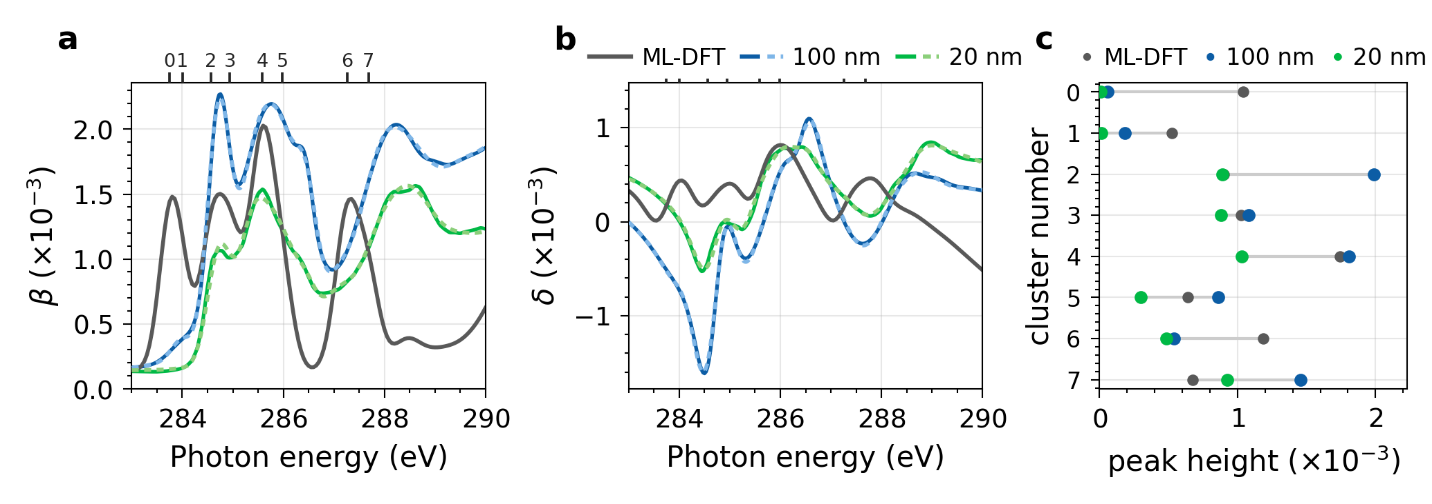
\includegraphics[width=\linewidth,height=0.75\textheight,keepaspectratio]{fig4.1_ML-DFT}
  \caption[Sample dependent NEXAFS for Alq\textsubscript{3}.]{Sample dependent NEXAFS for Alq\textsubscript{3}. (a) Imaginary refractive index component \(\beta(E)\) compared between samples of different deposition thicknesses presenting different spectral features along with ML clustered DFT calculations (gray). (b) KK calculated real refractive index component for the three different sources of \(\beta(E)\). (c) Peak amplitude difference map between the three models.}
  \label{fig:5.1}
\end{figure}



The dominant approach for constructing optical models for RSoXS originates from experimental measure of the NEXAFS spectroscopy on thin film standard samples of the material. The index of refraction \(n(E) = 1 - \delta(E) + i\beta(E)\) is found in pieces, \(\beta(E)\) is directly measured from the measured absorption spectra (\cref{fig:5.1}a), and \(\delta(E)\) is computed from the KK transformation (\cref{fig:5.1}b).\autocite{watts2014calculation,yan2013accurate} However, not all NEXAFS measurements probe the same absorptive response. In total electron yield mode (TEY) the incident X-ray beam excites only the top surface of the material, and electrons are collected through a conductive substrate, meaning the measured signal convolves surface effects with the material's own conductivity. For emergent materials bearing engineered optical and electronic properties, different preparations can drastically alter the measured NEXAFS spectra. Additionally, it is not always possible to form thin film standards, such is the case for organic solvents, metals bearing novel oxidation states, mixed phase interfaces, molecules in unstable conformations, and interface driven bonding hybridizations.

\Cref{fig:5.1} demonstrates this in thin vapor deposited films of Alq\textsubscript{3}, a common material platform used both as an electron transport and emissive layer in organic light-emitting devices, and in spintronic applications. Here we present two samples prepared under near identical conditions but with drastically different NEXAFS spectra. Notably within the \(\pi\) manifold where the relative peak intensities of all transitions vary strongly between samples, a response that is reflected similarly in \(\delta(E)\). In addition to this intensity only variation, a low energy transition at \qty{284}{eV} can be resolved in the thicker film but is entirely suppressed in the thin film NEXAFS. Machine learning clustered density functional theory (ML-DFT) calculations suggest the presence of a family of transitions at this energy capable of describing this feature. However, the presented spectra use the raw calculated transition energies with no static energy shifts, so the absolute energy scale is not well determined from DFT. A shift of \qty{+0.01}{eV} maximizes the alignment to the \qty{100}{nm} film, while a shift of \qty{0.8}{eV} would maximize alignment for the thinner \qty{20}{nm} sample, removing the possibility for the ML-DFT transitions to describe this \qty{284}{eV} transition, implying that this transition emerges as an effect of the thicker film and is not present in either a single molecule DFT calculation or within thinner films of the material. Regardless with the unshifted ML-DFT calculations, it is possible to refine the transition moments to a common set of transition clusters with only oscillator strength varying between the samples.

\section{The Spectral Basis}\label{sec:the-spectral-basis}

Optical responses in macroscopic molecular and polymer material systems emerge from their ensemble of molecules and polymers within the film. Assuming the packing characteristics of nearby molecules and polymer chains does not disrupt or alter the electronic states and excitation energies, then the individual molecular contributions sum linearly, weighted by their population representation within the ensemble. Generally, this can be expressed as the ensemble average over molecular configuration parameters \(\left\{ p_{i} \right\}\)

\begin{equation}
  n_{\mathrm{film}} = \left\langle n_{\mathrm{mol}} \right\rangle_{\{ p_{i} \}}.
  \label{eq:ensemble-average}
\end{equation}

Most commonly these handles molecular orientation degrees of freedom such as tilt angle or order parameters and packing characteristics such as density scaling. Multi component films are constructed similarly from an effective media approximation, but linear volume fraction weighted combinations is a good approximation for soft matter in the soft X-ray regime. Regardless this presents the key to transforming the molecular response into the film optical constants that are used to describe scattering.

The molecular resonant response can be decomposed into three regions, the non-resonant pre-edge, near edge fine structure, and the post edge. While the ionization phenomena that lead to the edge itself include nonlinear, multi electron and multi photon interactions, the edge description itself composeslinearly with the fine structure to describe the resonant response. Because of this, it can be separated from the fine structure

\begin{figure}
  \centering
  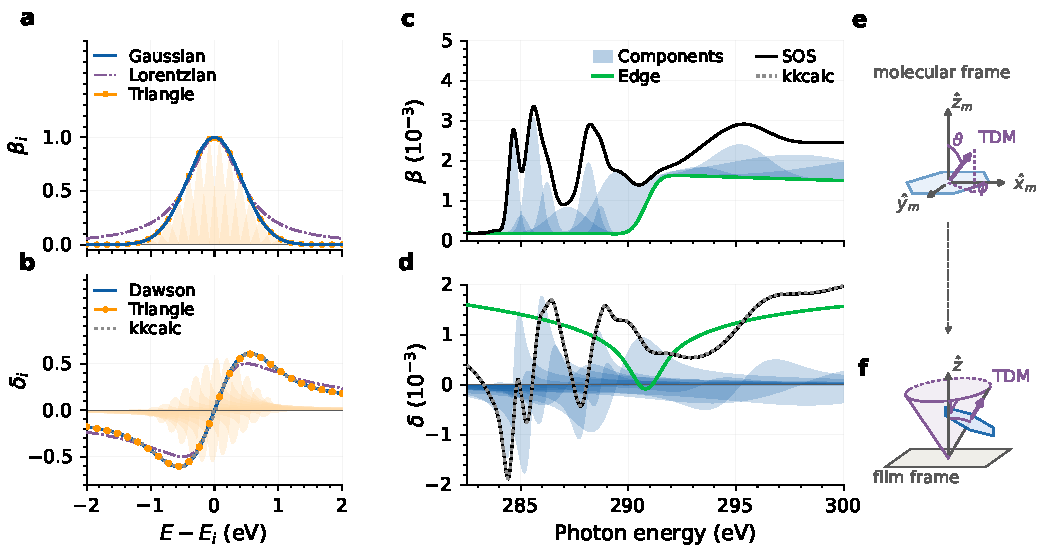
\includegraphics[width=\linewidth,height=0.75\textheight,keepaspectratio]{fig5-02_oscillator-basis}
  \caption[Gaussian spectral basis compared with a Lorentzian oscillator and triangle bases.]{(a) Spectral, Gaussian basis compared with Lorentzian damped driven oscillator and the sum of 26 triangle bases. (b) Sum over states approach constructing \(\beta(E)\) from the sum of Gaussian resonance building blocks, each originating from a refined ML-DFT cluster. (c) Derived \(\delta(E)\) computed directly from the sum of Dawson functions, overlayed the KK calculation of the results.}
  \label{fig:5.2}
\end{figure}


\begin{equation}
  n(E) = 1 - \left[ \delta_{\mathrm{edge}}(E) + i\beta_{\mathrm{edge}}(E) \right] + \sum_{i}\left[ \delta_{i}\left( E;\vec{\theta} \right) + i\beta_{i}\left( E;\vec{\theta} \right) \right],
  \label{eq:sos-index}
\end{equation}

where \(\beta_{i}\) is the absorption associated with a single resonant feature, and \(\delta_{i}\) its KK conjugate pair. This decomposition is commonly called a building block approach but is better described as a spectral decomposition as each resonant feature derives from the molecular quantum transitions. Each resonant feature represents an ensemble of quantum transitions from tightly bound atomic states to unoccupied molecular orbitals, so the line shape assumes the convolution of fundamental lifetime broadening and thermal broadening from the ensemble of transitions.\autocite{stohr2010nexafs} When lifetime broadening is dominant, resonant features follow the Lorentzian line shape derived from the textbook damped driven harmonic oscillator.\autocite{stohr2010nexafs,kuzyk2023nonlinear} Phenomenologically, this is rarely the case and ensemble broadening dominates resulting in a Gaussian line shape profile. While the real component \(\delta_{i}\) for the Lorentz oscillator can be derived from first principles, Gaussian bases require performing the KK transformation, resulting in the Dawson special function. This results in a functional pair

\begin{equation}
  \begin{gathered}
  \beta\left( E;E_{i},w_{i},A_{i} \right) = \frac{A_{i}}{w_{i}\sqrt{\pi}}\exp\left[ - \left( \frac{E - E_{i}}{w_{i}} \right)^{2} \right], \\
  \delta\left( E;E_{i},w_{i},A_{i} \right) = \frac{2A_{i}}{w_{i}\pi}D\left[ \frac{E - E_{i}}{w_{i}} \right],
  \end{gathered}
  \label{eq:gauss-dawson-pair}
\end{equation}

where \(w_{i} = \Gamma_{i}/(2\sqrt{\ln 2})\) for a given full width at half maximum \(\Gamma_{i}\), \(A_{i}\) the transition intensity, \(E_{i}\) the transition energy, and \(D\) the Dawson function.

This direct spectral decomposition presents directly interpretable parameters that map onto the individual quantum states associated with the resonant feature. The resonant energy immediately maps to the transition energy associated the quantum states, and the amplitude is directly proportional to the oscillator strength and TDM. Importantly, the transition intensity depends on the angle between the TDM orientation and the electric field polarization vector so that not only does this basis enforce the Kramers-Kronig relations, but it also enforces molecular, material, and dipole symmetries, producing the index of refraction tensor for free.

As a tensor the decomposition can now be augmented so that the peak amplitudes follow \(A_{i}\left( {\mu_{i},\vartheta}_{i},\varphi_{i} \right)\) where \(\vartheta_{i}\) and \(\varphi_{i}\) are the polar and azimuthal angles associated with the TDM orientation and \(\mu_{i}\) is the transition dipole moment amplitude (\cref{fig:5.2}e). This allows for the amplitude to be decomposed into an \(xx\), \(yy\), and \(zz\) component the full tensor. Projecting the transition dipole moment onto the lab frame through its polar and azimuthal angles gives \(A_{i,xx} = \mu_{i}^{2}\sin^{2}\vartheta_{i}\cos^{2}\varphi_{i}\), \(A_{i,yy} = \mu_{i}^{2}\sin^{2}\vartheta_{i}\sin^{2}\varphi_{i}\), and \(A_{i,zz} = \mu_{i}^{2}\cos^{2}\vartheta_{i}\). Once the dipole is described in the molecular reference frame each of the dipole orientations and their magnitude can be refined to match experimental results.

\section{Measuring Buried Electronic States}\label{sec:measuring-buried-electronic-states}

\begin{figure}[htp]
  \centering
  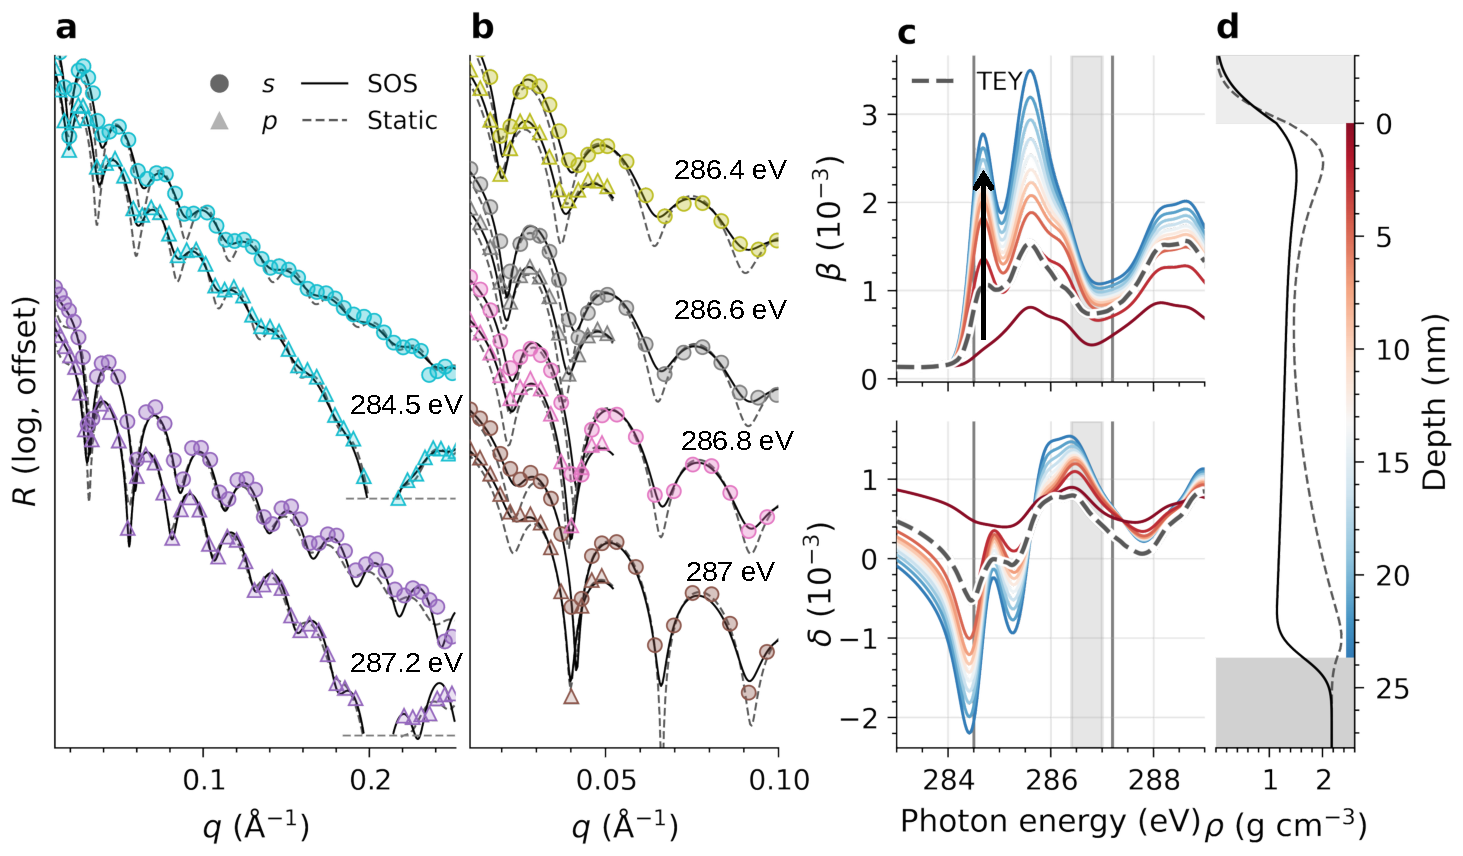
\includegraphics[width=\linewidth,height=0.75\textheight,keepaspectratio]{fig5-03_alq3-fit}
  \caption[Alq\textsubscript{3} reflectivity fit validating the resolved ML-DFT cluster model.]{Alq\textsubscript{3} reflectivity fit validating the resolved ML-DFT cluster model. (a) RSoXS reflectivity in s- and p-polarization at ten resonant energies (offset for clarity), with the resolved sum-over-states (SOS) model (solid) and the model fixed to the \qty{20}{nm}-film NEXAFS optical constant (dashed). (b) Expanded low-q region showing the SOS model tracking fringe positions and amplitudes that the \qty{20}{nm}-NEXAFS model misses. (c) Depth-resolved \(\beta(E)\) (top) and \(\delta(E)\) (bottom) recovered by the SOS model, colored by depth from the free surface to the substrate. (d) Density profile recovered by the SOS model (solid) compared with the \qty{20}{nm}-NEXAFS model (dashed), which is pushed to its fit bounds at the surface and in the bulk.}
  \label{fig:5.3}
\end{figure}

The Alq\textsubscript{3} optical model is defined by first refining the ML-DFT clusters to NEXAFS collected on the same sample (\cref{fig:5.1}). Peak amplitudes are then refined as a function of depth with widths and transition energies held fixed. The material structure is modeled with a single slab of Alq\textsubscript{3} with its density following a continuous exponential transition from the interface induced density at the surface and the free surface and substrate into the bulk of the film, with surface roughness modeled in the Névot-Croce sense.\autocite{heilman2026sub,nevot1980caracterisation} This approach uses pinning densities \(\rho_{Si}\ \&\ \rho_{Surf}\) with respective exponential characteristic thicknesses \(\tau_{Si}\ \&\ \tau_{Surf}\) along with the bulk properties \(\rho_{bulk}\), total thickness \(t\) and surface roughness \(\sigma_{r}\). The Alq\textsubscript{3} peak heights then vary over this same functional depth profile with bulk and interfacial pinned amplitudes for each refined peak, tying the electronic deviations within Alq\textsubscript{3} molecules to the packingcharacteristics set by the interfacial surface potentials, a feasible mechanism for measured depth dependent optical responses.



\Cref{fig:5.3} showcases the model fit results on RSoXS reflectivity measured at ALS beamline 11.0.1.2. High \(q\)-range measurements at 284.5 and \qty{287.2}{eV} (\cref{fig:5.3}a \& vertical lines in \cref{fig:5.3}c) maximize spatial resolution with the aim to capture small and buried structures and are captured at energies with low resonant absorption \(\beta\) and with opposite signs of \(\delta\). The shorter \(q\)-range measurements of \cref{fig:5.3}b aim to better capture the general spectral shape (shaded \cref{fig:5.3}c). Two optical models are compared, the static ML-DFT NEXAFS refined optical constants (dashed throughout) against the SOS depth dependent response (solid traces). The sum over states (SOS) model, uses 28 free parameters describing the evolution of five resonant transition amplitudes along the depth of the film, compared with the static model derived from NEXAFS collected on the same film. The resonance refinements improve the reduced \(\chi^{2}\) best fit statistic \(\chi_{\nu}^{2}\) from 63.1 to 12.9 and improves the BIC by 1527 (\cref{tab:5.1}), despite having more than twice as many free parameters. This is not the result of a single poorly described energy, the weighted RMSE of the NEXAFS-fixed model exceeds the SOS model at every one of the ten measured energies, roughly by a factor of two to three throughout the \(\pi^{*}\) manifold.

\begin{table}
  \centering
  \caption{Fit quality comparison between the SOS and static NEXAFS models.}\label{tab:5.1}
  \begin{tabular}{l S[table-format=2.0] S[table-format=2.1] S[table-format=1.2] S[table-format=4.0]}
    \toprule
    Model & {\(k\)} & {\(\chi^{2}_{\nu}\)} & {Weighted RMSE} & {\(\Delta\)BIC} \\
    \midrule
    SOS (5 peaks) & 28 & 12.9 & 3.55 & 0 \\
    TEY NEXAFS & 13 & 63.1 & 7.89 & 1527 \\
    \bottomrule
  \end{tabular}
\end{table}

The refined model reproduces both the measured \(\beta(E)\ \)and its KK-derived \(\delta(E)\) directly as a function of depth within the film (\cref{fig:5.3}c) derived as an evolution of resonant intensities along the depth of the film. Generally, these results describe an increase in absorption uniformly across all peaks as a function of depth, with the strongest absorption at the substrate interface. The static optical approach attempts and fails to capture this behavior using a strong density gradient pushing the density at the substrate to 2.5 times what its stoichiometry and packing geometry allow. The strongest evolution arises with the third resonance, nearly fully suppressed right at the vacuum surface, before growing substantially into the bulk and at the silicon interface. The origin of this evolution is not well understood and may arise from any of, hydrocarbon contamination at the surface so that this interfacial resonant state is a model hallucination, molecular conformation shifts that suppress the transition rates near the surface while enhancing them near the substrate, the surface potentials themselves altering the electronic structure leading to hybridization, or some other optical or electronic property of Alq\textsubscript{3} not characterized in these films. The challenge is that the present data only directly measures the optical constants at the energies probed with the optical constants at other energies inferred based on the dispersive properties of each resonant transition, with most of this out of measurement sensitivity originating from \(\delta(E)\). To properly investigate the source of the depth dependent optical evolution; better sampling strategies are needed to improve the reliability of these measured optical constants.

\section{Tracing Dipole Evolution with Depth}\label{sec:tracing-dipole-evolution-with-depth}

\begin{figure}[htp]
  \centering
  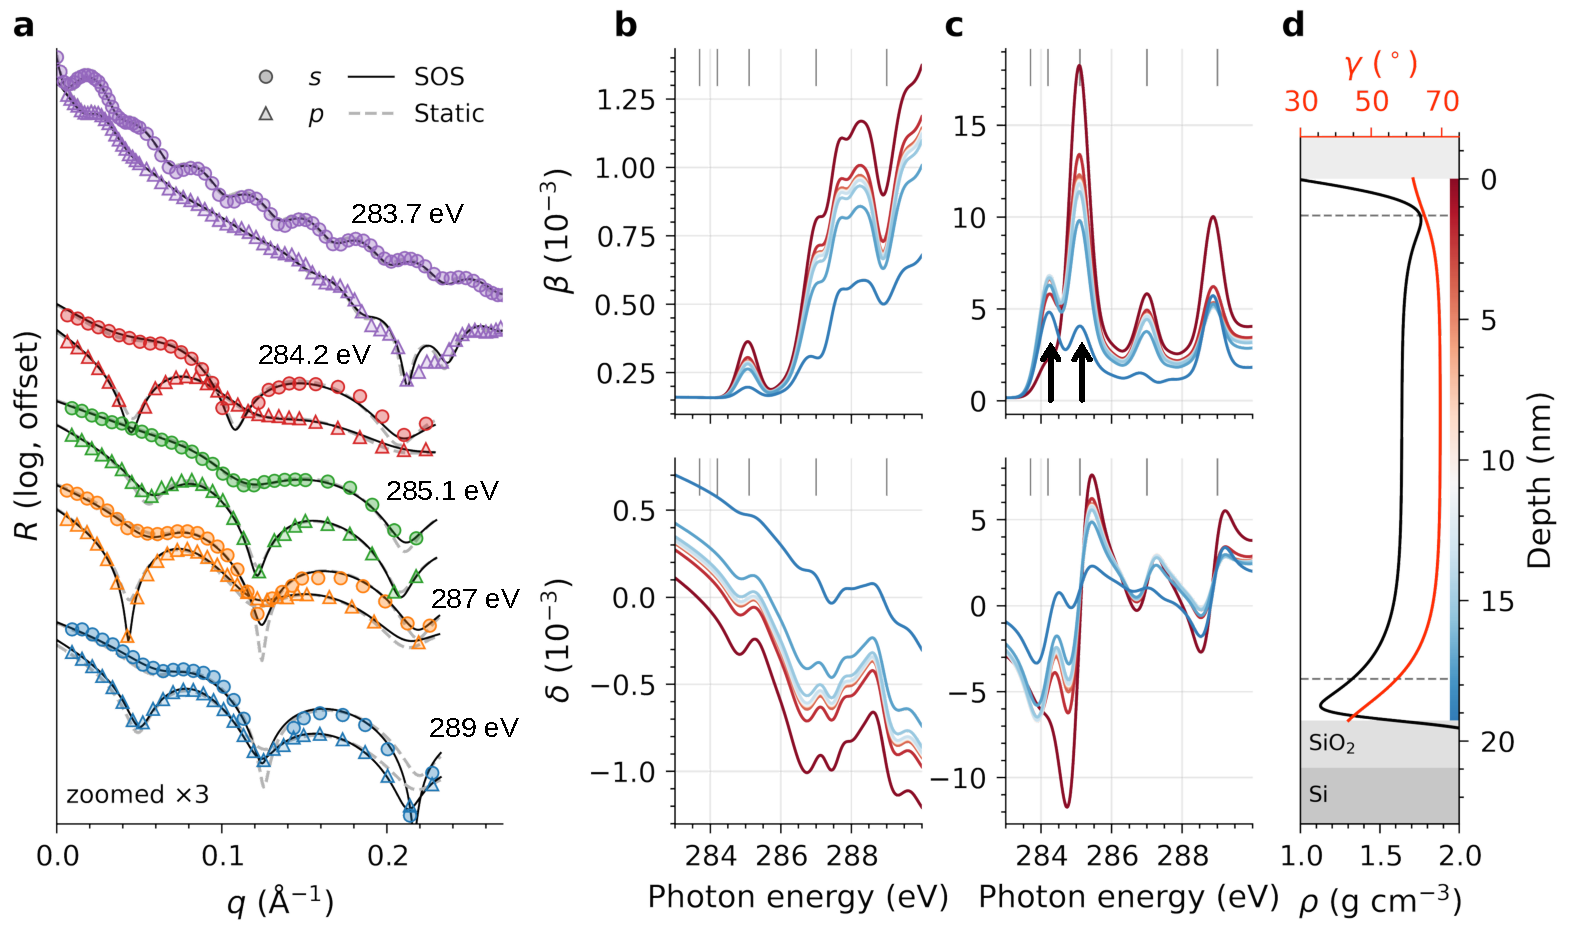
\includegraphics[width=\linewidth,height=0.75\textheight,keepaspectratio]{fig5-04_znpc-tdm-depth}
  \caption[Depth-resolved transition dipole moment orientation in ZnPc.]{Depth-resolved transition dipole moment orientation in ZnPc. (a) P-RSoXR reflectivity (zoomed ×3, offset for clarity) at five resonant energies in s- and p-polarization, with the resolved sum-over-states (SOS) fit (black) and a NEXAFS-fixed fit (gray). (b) Molecular xx and (c) molecular zz tensor components of \(\beta(E)\) (top) and \(\delta(E)\) (bottom) recovered by the SOS model at each sampled depth (colorbar). (d) Density profile \(\rho(z)\) (solid, bottom axis) and the resolved TDM tilt angle \(\gamma(z)\) (dashed, top axis), with the free-surface and SiO\textsubscript{2}/Si substrate regions shaded.}
  \label{fig:5.4}
\end{figure}

Next, we demonstrate the approach for tracking individual dipole orientations along the depth of the film. Zinc phthalocyanine (ZnPc) is a well-studied molecular platform that forms novel interfacial molecular states when deposited on silicon.\autocite{heilman2026sub} Additionally, the ML-DFT tensor of ZnPc reproduces angle-resolved NEXAFS of these films with an average error of 2.7 percent and, with a single tilt and density at each depth, describes their polarized reflectivity at every measured energy (\cref{chap:znpc}).\autocite{murcia2026quantitative,heilman2026sub} Moreover, PVD can easily produce highly anisotropic films, contrary to Alq\textsubscript{3} making it a natural platform to evaluate capability for this technique to track the TDM orientation of individual dipoles along with the molecular orientation as a function of depth within thin films.



\Cref{fig:5.4}a shows polarized reflectivity captured from \qty{20}{nm} thin films of ZnPc deposited on bare silicon (the film of \cref{chap:znpc}\autocite{heilman2026sub}). Following the similar convention described above, a long q-range measurement is performed at \qty{283.7}{eV} with low absorption, yet this time directly probing the energies of the four most prominent resonances within the \(\pi\) manifold (ticks, \cref{fig:5.4}). The structural model follows the same single slab continuous profile as previously published, with the orientation and density at the surface and substrate interfaces set by their respective surface potentials, with orientation and density relaxing into the bulk. The optics are then extended by also fitting the TDM amplitude of each of the four primary resonant transitions, with depth dependence set by the total thickness \(t\) and same characteristic interfacial thicknesses \(\tau_{Si}\ \&\ \tau_{Surf}\). The molecular optical tensor is highly uniaxial, so each TDM is symmetrized fitting only the polar cone angle \(\vartheta\ \)for each of these four resonances. In the fits reported here each cone angle is held constant with depth, so peak amplitudes vary over the film while the tensor projection of each resonance changes with depth only through the molecular tilt profile of \cref{chap:znpc}. As with Alq\textsubscript{3}, the resolved model is checked against a conventional NEXAFS-fixed alternative. \Cref{tab:5.2} compares the two fits to the \(N = 745\) point ZnPc reflectivity dataset shown above (\qty{283.7}{eV} and four resonant energies, s and p polarization, measured counting-statistics errors, fit on log-reflectivity residuals). model again fits markedly better, χ²ν = 3.63 against 10.33 and ΔBIC = 690 in its favor, but the per-energy residuals show a different pattern than Alq\textsubscript{3}: the two models agree closely at the lower three energies and diverge sharply only at 287.0 and \qty{289.0}{eV}, where the NEXAFS-fixed weighted RMSE more than doubles. These are the energies carrying the strongest TDM-orientation sensitivity in this molecule, so the conventional model is adequate where orientation contrast is weak and fails specifically where it is strong, rather than failing uniformly.

\begin{table}
  \centering
  \caption{Fit quality comparison between the SOS and static NEXAFS models.}\label{tab:5.2}
  \begin{tabular}{l S[table-format=2.0] S[table-format=2.2] S[table-format=1.2] S[table-format=3.0]}
    \toprule
    Model & {\(k\)} & {\(\chi^{2}_{\nu}\)} & {Weighted RMSE} & {\(\Delta\)BIC} \\
    \midrule
    SOS (4 peaks) & 37 & 3.63 & 1.86 & 0 \\
    NEXAFS & 21 & 10.33 & 3.17 & 690 \\
    \bottomrule
  \end{tabular}
\end{table}

Four resonances were opened in the fit, numbered 1 to 4 in order of energy at 284.2, 285.1, 287.1, and \qty{288.9}{eV}, with the molecular tilt and density held at the \cref{chap:znpc} gradient values (\ang{58.7}, \ang{69.6}, and \ang{38.4} and 2.05, 1.64, and \qty{0.87}{g.cm^{-3}} at the vacuum surface, in the bulk, and at the SiO\(_{2}\) interface). Dividing each fitted height by the local density and by its NEXAFS-refined amplitude gives a per-molecule oscillator strength relative to NEXAFS. The two lowest \(\pi^{*}\) resonances carry the largest oscillator strength and move in opposite directions. At the vacuum surface resonance 1 falls to 0.30 of its NEXAFS value while resonance 2 rises to 1.45, and at the SiO\(_{2}\) interface resonance 1 rises to 1.65 while resonance 2 falls to 0.67, so between the two boundaries resonance 1 grows 5.5-fold and resonance 2 halves. Their summed strength stays within 4 percent of the NEXAFS value at both boundaries (1.04 at vacuum, 1.02 at SiO\(_{2}\)) and rises to 1.19 in the bulk, an excess reported with the caveat that density and tilt are fixed at the \cref{chap:znpc} values. Resonance 3 is unchanged at the surface and in the bulk (0.95) and falls to 0.25 at the interface, and resonance 4 changes most in relative terms, reaching 2.90 at the interface where the \(\pi^{*}\) manifold meets the \(\sigma^{*}\) onset. Each opened resonance carries one cone angle, constant with depth. The \(\pi^{*}\) angles stay within \ang{9} of the ring normal (resonance 1 from \ang{3.0} in the NEXAFS refinement to \ang{0.0}, resonance 2 from \ang{0.9} to \ang{8.9}), while resonance 3 moves from \ang{28.5} to \ang{24.6} and resonance 4 from \ang{26.0} to \ang{12.3}, so the largest reorientation relative to NEXAFS also occurs at the \(\pi^{*}\) to \(\sigma^{*}\) boundary.

In the ML-DFT clusters, resonance 1 is dominated by 1s excitation of carbon site C2 into the lowest unoccupied orbital (MO 117), and resonance 2 by excitation of site C3 into a higher \(\pi^{*}\) orbital (MO 119), both benzo-ring carbons, while resonance 4 arises from site C1, the pyrrole carbon bound to nitrogen, whose 1s ionization potential lies \qty{1.5}{eV} above the benzo carbons (site labels as in Supplemental Material). Because the structural model already fixes the local density, we surmise that the anti-correlated change of resonance 1 and resonance 2 at the two interfaces, with a nearly conserved sum, is a redistribution of spectral weight between the two lowest unoccupied states rather than a change in the number of absorbing molecules. Three mechanisms could produce it, each with a different signature. Hybridization or charge transfer at the SiO\(_{2}\) interface would perturb the LUMO most where molecules contact the oxide, confining the change to the first molecular layers and shifting the transition energy as well as its strength. Packing-dependent \(\pi\) overlap tied to the tilt gradient would scale the reweighting with the local tilt \(\gamma(z)\), so the same ratio of resonance 1 to resonance 2 should recur wherever the tilt is the same. Disorder at the free surface would broaden the resonances and lower the anisotropy of every transition rather than exchange weight between two. A refit that frees each cone angle separately at the surface, in the bulk, and at the interface, together with a fixed-angle energy scan from 283 to \qty{290}{eV} at several incident angles, would separate these, since only the first predicts an energy shift and only the second ties the reweighting to \(\gamma(z)\).

These results also open a route to refining the ML-DFT clusters themselves, using the clusters as computed by the clustering routine as priors for the spectral analysis. The energetic uncertainties of the present datasets are too large for this, and fixed-angle reflectivity across the edge at one or more incident angles, measured with this aim, may suffice.

\section{Energetic Sampling Efficiency}\label{sec:energetic-sampling-efficiency}

\begin{figure}[htp]
  \centering
  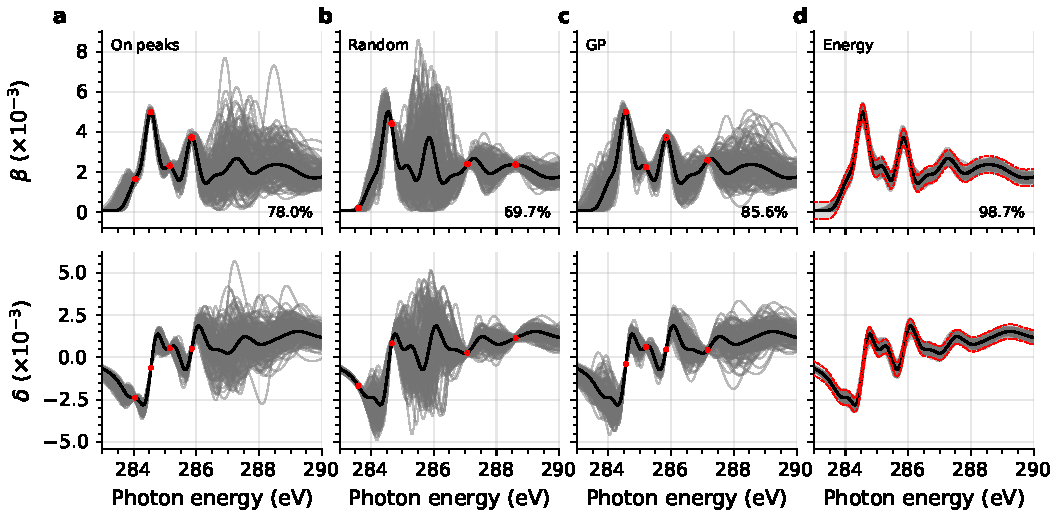
\includegraphics[width=\linewidth,height=0.75\textheight,keepaspectratio]{fig5-05_energy-sampling}
  \caption[Monte-Carlo sampling of resonant transitions for polystyrene (C\textsubscript{8}H\textsubscript{8}).]{Monte-Carlo sampling of resonant transitions for polystyrene (C\textsubscript{8}H\textsubscript{8}). Generated \(\beta(E)\) (a) and conjugate \(\delta(E)\) (b) traces over flat priors. Circles indicate fixed energy measurement that perfectly determine both δ and β at a given energy though measurement simulating RSoXS analysis at that energy. Remaining traces are NEXAFS profiles that agree at the measured energies with the ground truth in bold.}
  \label{fig:5.5}
\end{figure}



One natural consequence of this analysis is a framework for generating feasible, KK-consistent optical constants and tensors. The number of peaks, along with their heights, widths, and transition energies, can be sampled over a realistic parameter domain, with the optical response composed from their sum. This approach may be useful for generating training data in machine learning, and it also presents a natural way to explore sampling strategies and measurement uncertainty within resonant techniques, as is done in \cref{fig:5.5}. A synthetic model of ten carbon K-edge transitions on a fixed bare-atom continuum (constructed for a stoichiometry of C\textsubscript{8}H\textsubscript{8}) serves as the ground truth. Transition energies are drawn from Gaussian priors, and widths and heights from log-normal priors, centered on the ground truth. Each sampling strategy aims to measure \(\beta\) and \(\delta\) at its chosen energies within a Gaussian error of \(\sigma\  = \ 10⁻⁴\), simulating a sparse RSoXS measurement that precisely extracts optical constants at only a few energies. The family of \(\beta(E)\) and \(\delta(E)\) curves consistent with those measurements is then drawn from the Bayesian posterior by Markov chain Monte Carlo. All curves agree with the measurement error but diverge between them, visualizing the uncertainty a given energy sampling leaves unresolved. We quantify this with the fractional reduction, relative to the prior, of the variance in the complex index \(n\  = \ 1\  - \ \delta\  + \ i\beta\) integrated over 283 to \qty{290}{eV}.

Three of the four strategies measure four energies. The first places them on the leading resonance centers (\cref{fig:5.5}a). The second draws them uniformly at random (\cref{fig:5.5}b). The third selects them greedily with a Gaussian process whose kernel is the prior covariance of \(\beta\) and \(\delta,\) with each energy chosen to maximize the expected drop in variance given the earlier picks (\cref{fig:5.5}c). The fourth is a continuous energy scan in \qty{0.1}{eV} steps across the same window (\cref{fig:5.5}d) but using a wider uncertainty to simulate an energy scan such as a fixed angle reflectivity measurement. Measuring on the resonances reduces the variance by 78.0\%, but above \qty{286}{eV} the posterior traces fan out freely in both \(\beta\) and \(\delta\). The random set shown reduces it by 69.7\% and leaves the 285 to \qty{286.5}{eV} region unconstrained. This seed is favorable. Across 200 random energy sets, a linear-response estimate gives 53 ± 19\%. The Gaussian-process design moves one point onto the flank between resonances at \qty{285.2}{eV} and another out to \qty{287.2}{eV}, raising the reduction to 85.6\%. Even so, four energies supply eight observables against 30 transition parameters. Under the same linear-response estimate, a tenfold improvement in precision leaves the on-resonance reduction unchanged near 83\%. The equal-dose energy scan reaches 98.7\% despite its higher per-point noise.

For sparse RSoXS measurements, the limit is therefore set by the number of energies and not the precision at a single energy. Even exact knowledge of β and δ at four energies leaves the spectrum between them undetermined, with an optimized choice of energies recovering only part of that gap. We surmise that a model-based analysis of sparse-energy RSoXS should therefore be anchored to a continuous energy dependent scan even if each measurement over the scan has higher measurement noise and resolves \(\delta\) and \(\beta\) to a lower precision. Short of that, the same sampling framework can be used to choose measurement energies before a beamtime, extending traditional ideas selecting energies based on contrast.

\section{Discussion}\label{sec:discussion}

The Alq\textsubscript{3} and ZnPc case studies demonstrate the same effect from two different directions. In Alq\textsubscript{3}, replacing a single borrowed NEXAFS optical constant with independently refined resonant-feature heights removes a degeneracy between optical model and film density that the simpler model had been resolving by pushing density to an unphysical value. In ZnPc, replacing a single borrowed tensor with per-resonance cone angles and depth-resolved amplitudes reveals that different transitions reorient to different degrees relative to their NEXAFS-refined values and that the two lowest π* resonances exchange spectral weight between the two interfaces, a distinction the rigid model cannot express at all. Neither result follows from overfitting and both follow from adding optical degrees of freedom selectively to the independent resonances that poorly describe the measured signal. Tracking these resonances through the depth of the film then exposes physics, such as changes in packing or hybridization near an interface, that no single reference spectrum can capture.

Nothing in this spectral-decomposition framework is specific to Alq\textsubscript{3}, ZnPc, or small molecules, and the same analysis applies to any film, molecular, polymeric, or otherwise. All that is needed is a prior guess of the number of peaks needed to describe the optical response, and measurements dense enough in energy to constrain the optics across an absorption edge. By comparing model performance metrics including performance against non-fit validation data between best fit models constructed under different priors, it is possible to construct the optical constants directly without the need for the predefined resonant peaks that are taken here from the ML-DFT calculations. However, without these calculations, additional analysis on the final extracted resonant spectra is needed to understand the source of the electronic evolution throughout a film.

\section{Conclusion}\label{sec:conclusion}

We have presented a spectral decomposition of the optical response into Kramers-Kronig consistent oscillators tied to ML-DFT transition clusters, which refines the optical constants of buried regions together with the film structure. Because the parameter count is set by the number of resonances and not by the number of measured energies, resonant reflectivity becomes a direct probe of electronic states that no reference measurement reaches, extending its role beyond contrast variation. In Alq\textsubscript{3} the depth-dependent amplitudes remove a degeneracy between the optical model and the film density that the NEXAFS-fixed model could resolve only by driving the substrate density to an unphysical value. In ZnPc the per-resonance amplitudes and cone angles markedly improve the fit and show the two lowest π* resonances exchanging oscillator strength between the free surface and the oxide interface while their sum is nearly conserved. The sampling study shows that for sparse-energy measurements the number and placement of energies, and not the precision at each, limit the recovered spectrum, so continuous energy scans should anchor future analyses. Each refined resonance traces back to a family of electronic transitions, so the origin of its evolution with depth can be interrogated directly from the optical model, opening a route to depth-resolved spectroscopy of buried molecular layers.

\section{Methods}\label{sec:methods-1}

\textbf{Density functional theory:} A time independent transition potential calculation using the StoBe library was performed on a single molecule of ZnPc and Alq\textsubscript{3}. A HCH approach sets the manifold of transition energies, along with each TDM and oscillator strength, while the \(\Delta KS\ \)method is used to fix the absolute energy associated with each transition. For details see our previous work.\autocite{murcia2026quantitative} The ZnPc molecular geometry was extracted from a crystallographic structure file (.cif)\autocite{mai2020data} while Alq\textsubscript{3} used a thermally relaxed structure computed with UFF minimization.

Clustering was performed using the dft-learn implementation of the clustering routine from Murcia et.al. using energetic overlap to identify transitions.\autocite{murcia2026quantitative,victormurcia2025wsu} Oscillator strength threshold is determined using an elbow method. Overlap percentage is determined using a Bayesian Information analysis to select a percentage that produces the smallest set of clusters that best describe the original DFT calculation.

\textbf{Film growth and pre-characterization:} ZnPc samples were grown by physical vapor deposition under the same conditions described in prior work.\autocite{heilman2026sub} Small molecule ZnPc (C32H16N8Zn sourced from Sigma Aldrich) with purity \(\geq 99.5\%\) was further purified in the physical vapor deposition (PVD) chamber (base pressure \(< 1 \times 10^{- 7}\) Torr) by gradually heating, approaching ZnPc sublimation temperature over approximately an hour until no further off gassing of contaminants were detected by the quartz crystal monitor (QCM). Thin films (\({\sim}\)\qty{20}{nm} measured by QCM) of ZnPc were deposited at \(.2\ \mathring{\mathrm{A}}/s\) on high conductivity polished Si wafers (University Wafers). Wafers were cleaved \qty{1}{cm} x \qty{3}{cm} and cleaned via sonication in deionized water, acetone and isopropyl alcohols before a 30 min UV ozone bake. ZnPc was deposited onto these wafers. Alq\textsubscript{3} samples were grown by physical vapor deposition under similar conditions described in prior work.\autocite{ferron2023composition} Sublimation grade (99.995\% trace metals basis) Alq\textsubscript{3} was purchased from Sigma-Aldrich and deposited onto silicon substrates. Wafers were cleaved to and precleaned under the same conditions. Deposition was performed with the same base pressure and with thickness monitored to achieve \qty{24}{nm} of film growth.

\textbf{NEXAFS Collection:} ZnPc NEXAFS measurement methods are described in prior work with data taken from X-ray Atlas.\autocite{heilman2026x} Alq\textsubscript{3} NEXAFS on the \qty{200}{nm} sample are described in prior work with data taken from X-ray Atlas.\autocite{ferron2023composition} NEXAFS on the Alq\textsubscript{3} films studied independently though resonant reflectivity was performed in TEY mode at ALS beamline 11.0.1.2. Incident angles 30, 55 and 70 degrees demonstrate no dichroism within the film, consistent with DFT calculations.

\textbf{RSoXS Collection:} Polarized resonant soft x-ray reflectivity was measured at beamline 11.0.1.2 of the Advanced Light Source, Lawrence Berkeley National Laboratory, following the procedure established by Ferron et al.\autocite{ferron2023composition} Samples are transferred from inert storage to the end station where specular reflectance is captured on the CCD area detector with thermoelectric cooling. The sample surface is aligned to the goniometer axis of rotation by an iterative process that refines the sample rotation and height. Incident flux was attenuated using the scatter slits together with the higher order suppressor to avoid detector damage. Because the total reflectance varies by more than the detectors dynamic range, reflectivity is captured in overlapping \(\mathbf{q}\) subsets with suppressor settings and exposure time raised at each boundary once reflectivity reaches the noise floor. Data is collected first in s polarization and then in p polarization beginning at \qty{250}{eV}, below the carbon K edge, and stepping upward through the resonance. Upon polarization change, optics were allowed to re-equilibrate to the new heat load for 30 min before alignment was recalibrated. Photon energy was calibrated against the transmission NEXAFS of a polystyrene standard as well as electron yield on highly oriented pyrolytic graphite at the beginning and at the end of the shift with no discernable shift, bounding the energy drift over the experiment to the width of the primary polystyrene feature.

\textbf{Reflectivity modeling and fitting.} Reflectivity was computed with the 4 × 4 transfer matrix of refloxide and fit with refnx objectives.\autocite{alsrsoxsrefloxide2026als,nelson2019textless} For Alq\textsubscript{3} the film is a single slab whose density relaxes exponentially from pinned surface and substrate values into the bulk, with Névot-Croce roughness, and the fit is made on \(Rq^{4}\). For ZnPc the structure of \cref{chap:znpc} (tilt and density gradients, oxide, and substrate) is held fixed, and the fit frees the per-energy s and p scale factors and angle offsets, a global energy offset (refined to \(- 0.09\) eV), the heights of the opened resonances at the vacuum surface, in the bulk, and at the substrate, each bounded within 0.25 to 4 times its seed and non-negative at every depth, and one cone angle per opened resonance. Resonances were opened where they lie nearest the measured resonant energies. The data are the published ZnPc reflectivity at 283.7, 284.2, 285.1, 287.0, and \qty{289.0}{eV} in s and p polarization with measured uncertainties, fit on \(\log R\) by local least squares from the published graded fit, without a global search. The sampling study used Gaussian priors on transition energies and log-normal priors on widths and heights, a measurement error \(\sigma = 10^{- 4}\) on \(\beta\) and \(\delta\), posterior draws by MCMC, and a linear-response estimate over 200 random energy sets.

\chapter{X-ray Atlas -- An Open Science Project for Optical Constants}\label{chap:xray-atlas}

Prepared for submission to an academic journal.

Harlan Heilman, Obaid Alqahtani, Awwad Alotaibi, Victor Murcia, Zhong Xiaowei, Jeromy James Rech, Guillaume Freychet, Priyanka Ketkar, Thomas Ferron, Eliot Gann, Matt Gerbert, Lars Thomsen, Christopher R. McNeill, Alexander Hexemer, Dean M. DeLongchamp, Wei You, Cheng Wang, and Brian A. Collins, In Prep. (2026)

\section{Attributions}\label{sec:attributions-2}

B.C. and O.A. conceived the study. O.A., A.A., V.M., E.G., L.T., and T.F. collected, analyzed, and processed the initial data upload. J.J.R. and Z.X. synthesized polymer materials and aided H.H. in designing the molecule registry schema. T.F., E.G., M.G., C.R.M., A.H., D.M.D., W.Y., and C.W. worked with H.H. to design the NEXAFS schema, interaction, and analysis integration systems. H.H. wrote all code associated with the backend and front-end design and implementation of the database and wrote the manuscript with input from all authors.

\section{Background and Summary}\label{sec:background-and-summary}

Resonant elastic and inelastic X-ray scattering techniques depend on optical constants that are derived from a material's near edge X-ray absorption fine structure (NEXAFS), typically measured independently of the scattering experiment itself.\autocite{yan2013accurate,watts2014calculation} The index of refraction entering a diffraction, reflectivity or scattering calculation carries whatever noise, miscalibration, or normalization artifact is present in the spectrum it was derived from, so a model built on a poorly measured NEXAFS spectrum inherits those defects. Remeasuring NEXAFS on every sample ahead of a scattering measurement is time consuming and not always feasible, particularly for multicomponent blends and layered films, so researchers need a way to judge an existing measurement before deciding whether to reuse it, rederive it, or collect a new one. This requires seeing the raw measurement alongside quality information sufficient to make that judgment, not only the optical constants calculated from it.

Existing resources address parts of this problem. Individual dataset repositories released alongside a single publication, for example the calibrated NEXAFS spectra for common polymers released by Dhez, Ade, and Urquhart,\autocite{dhez2003calibrated} make spectra available but not programmatically accessible or interoperable with other repositories storing the same kind of data, so each repository requires its own bespoke tooling and meta-analyses across repositories are difficult. Platforms such as RefXAS\autocite{paripsa2024refxas} and the XASDB\autocite{chen2021database} database present queryable stores for hard X-ray absorption spectra but have limited applicability to the molecular and polymer materials that dominate resonant soft X-ray scattering, and most organic films carry optical anisotropy that only polarization dependent, angle resolved NEXAFS can quantify, which these hard X-ray databases do not collect. The Materials Project\autocite{horton2025accelerated} occupies a different position again, hosting computed K-edge XANES spectra for tens of thousands of inorganic materials, generated from relaxed crystal structures rather than measured from deposited films, with no polarization dependence recorded even where a molecular species is present.

Addressing what these efforts leave open means solving several problems together rather than providing a place to upload files. A usable store of resonant X-ray optical models needs the raw spectrum and its derived optical constants held together as linked records, so a user can trace a tensor back to the measurement it came from and judge both at once; a shared normalization and processing convention, so spectra collected on different beamlines are directly comparable rather than merely co-located; a standardized representation of the optical constants themselves, reported as the real and imaginary parts of the index of refraction rather than left to each author's choice of dielectric function or absorption cross section; quantitative data quality metrics that replace visual inspection with an objective, reproducible basis for judging a spectrum's signal to noise ratio, energy resolution, and normalization residual; full provenance, carrying a dataset's instrument, sample preparation, and processing history forward so a result can be traced back to and reproduced from its original configuration; and a model of attribution that credits every contributor to a dataset's collection, processing, and derivation, not only the author of the paper it eventually supports.

X-ray Atlas is built around these requirements. It stores raw NEXAFS measurements and the optical constants derived from them as linked, versioned records, scores every contributed dataset against automated quality metrics, validates structural requirements at the time of upload, and deposits each dataset version to Zenodo under a persistent, versioned DOI. It reaches toward a further goal still in development, acting as a single point of access to the wider ecosystem of X-ray spectral resources by surfacing or linking the Materials Project, RefXAS, and similar repositories from within the same search a user runs against its own holdings, so a researcher need not already know which of several disconnected repositories holds the data they want.

Within this dissertation the database answers a need that the preceding chapters expose. The optical model of \cref{chap:znpc} starts from an angle-resolved NEXAFS dataset of ZnPc deposited in X-ray Atlas (accession 193bc0c5), and \cref{chap:resonances} shows that NEXAFS of Alq\textsubscript{3} films prepared under nearly identical conditions differs in relative peak intensities and in a transition near \qty{284}{eV}. A spectrum taken from elsewhere must therefore be judged before it is reused, with any analysis built on it traceable to the exact revision it used.

\section{Methods}\label{sec:atlas-methods}

\begin{figure}[htp]
  \centering
  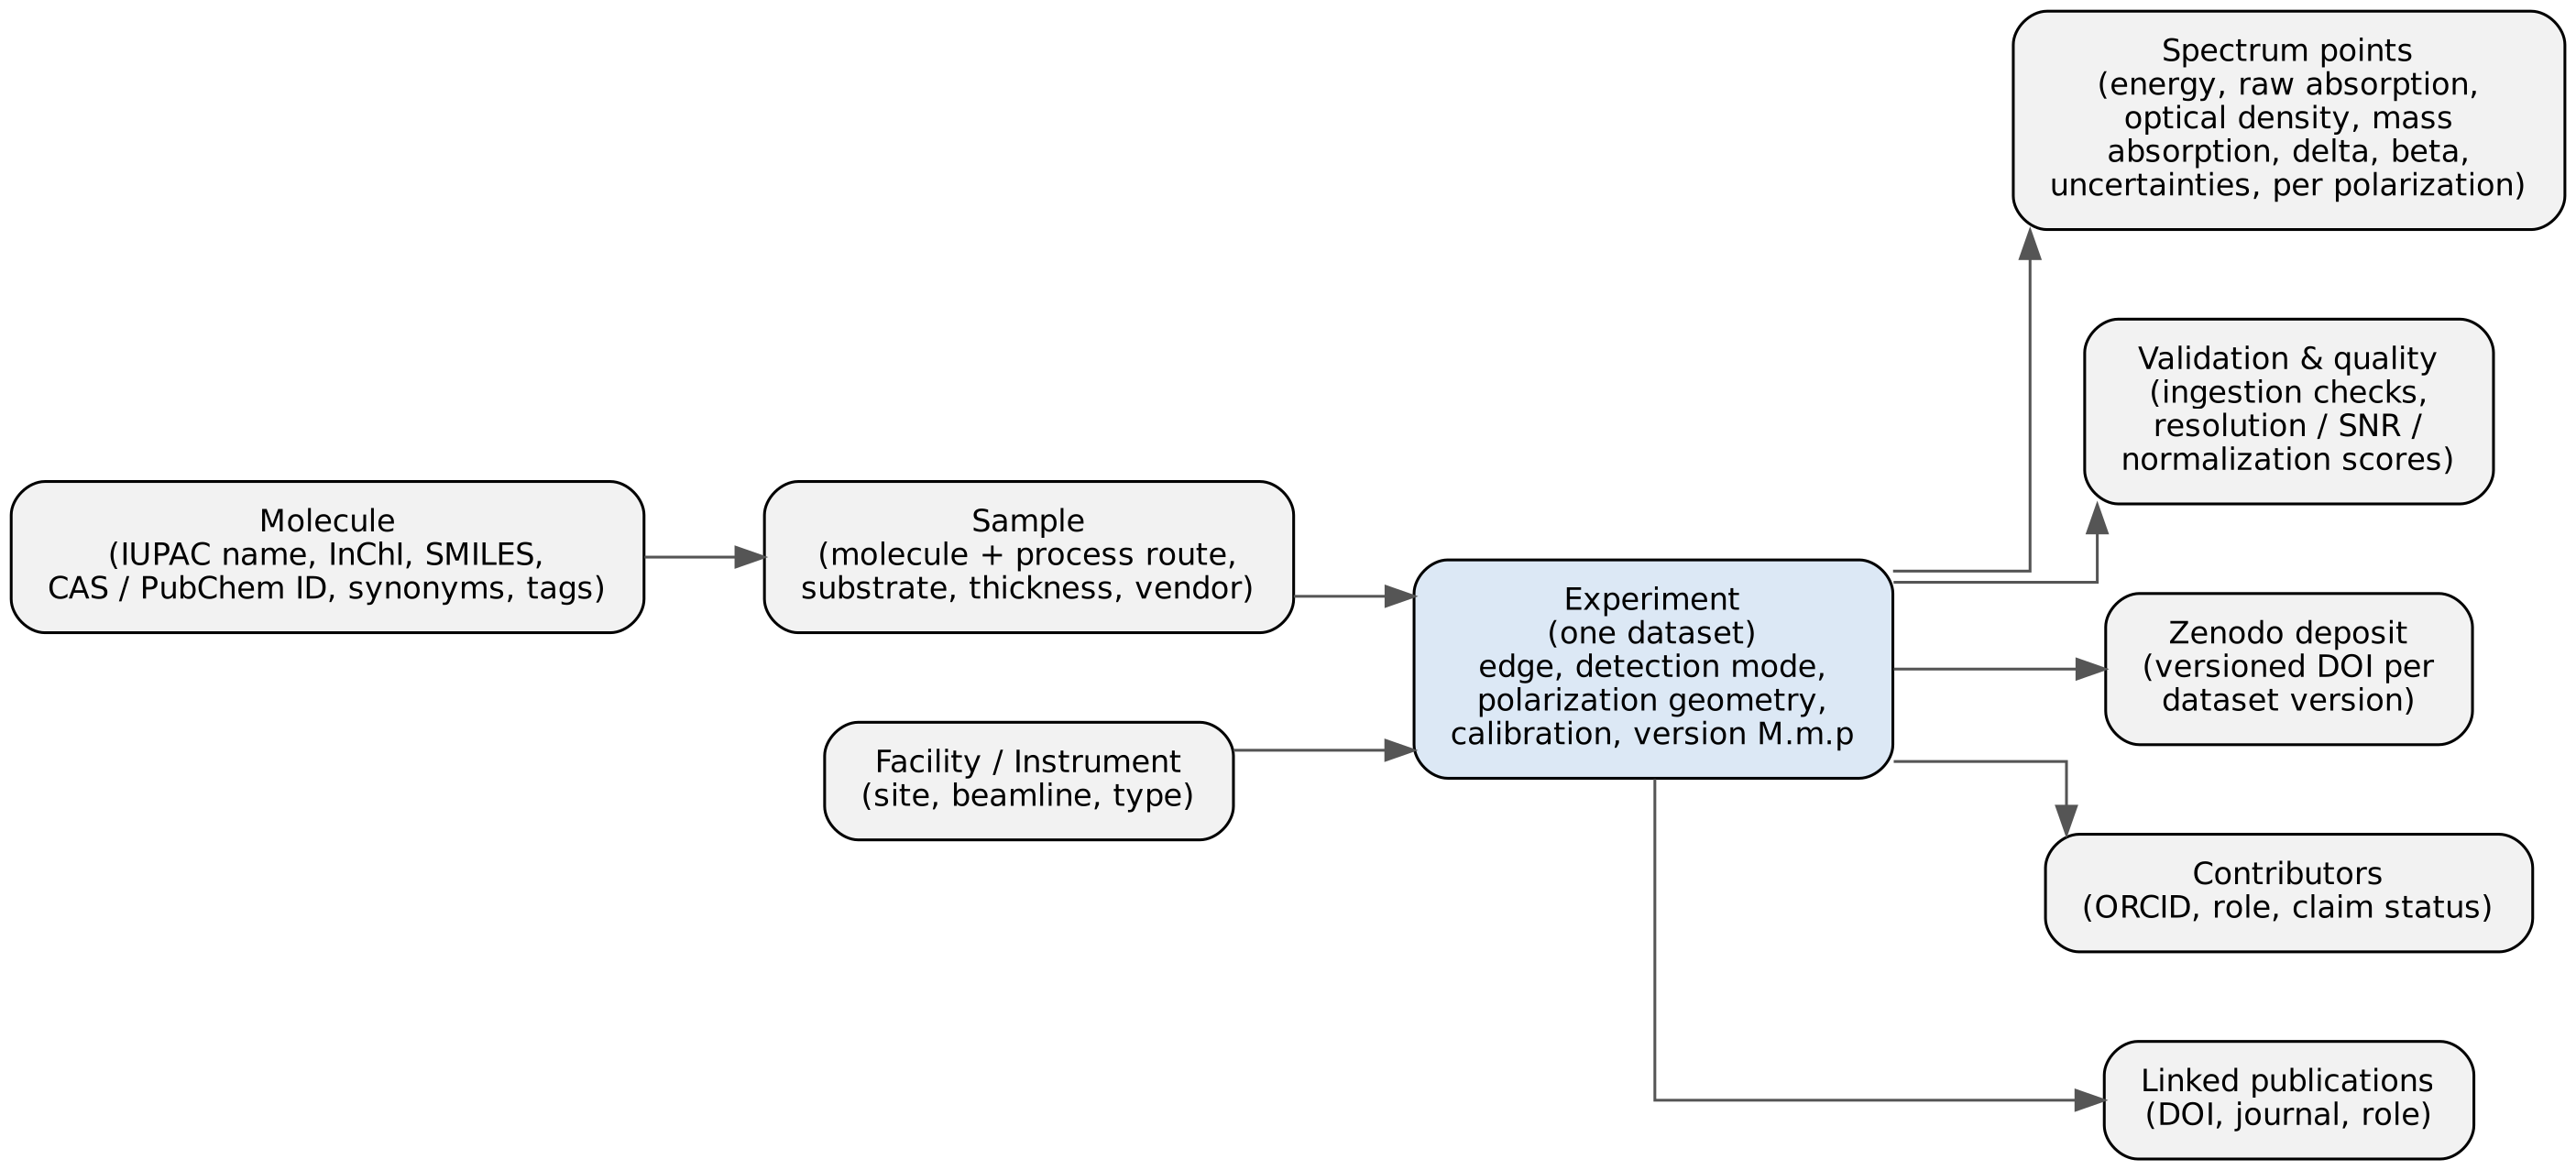
\includegraphics[width=0.95\linewidth,height=0.75\textheight,keepaspectratio]{fig6-01_data-model}
  \caption[Simplified entity relationship diagram of the X-ray Atlas data model.]{Simplified entity relationship diagram of the X-ray Atlas data model. Boxes correspond to the record types a user queries; the production schema normalizes several of these into additional tables for workflow and provenance tracking.}
  \label{fig:6.1}
\end{figure}



\textbf{Simplified data model.} X-ray Atlas is implemented as a relational database whose full schema spans more than twenty tables, most of which exist for workflow bookkeeping (collaboration permissions, background synchronization queues, dashboard caches) rather than for the scientific record itself. \Cref{fig:6.1} collapses that implementation schema to the eight record types a user of the data queries against. A molecule record carries chemical identity (IUPAC name, InChI, SMILES, chemical formula, CAS number, PubChem CID, and searchable synonyms); a sample record links a molecule to a physical specimen through its processing route (dry or solvent deposition method, solvent, substrate, patterning layer, nominal thickness, vendor); an experiment record is one dataset, carrying the facility and instrument it was collected on, the absorption edge (target atom and core level), the detection mode (total electron yield, partial electron yield, fluorescence yield, or transmission), the polarization geometry, the calibrationmethod, and a three part version number; spectrum point records carry the measured quantities themselves, one row per photon energy per polarization geometry. Validation and quality records, Zenodo deposit records, contributor records, and linked publication records attach to each experiment and are described below.

\begin{figure}
  \centering
  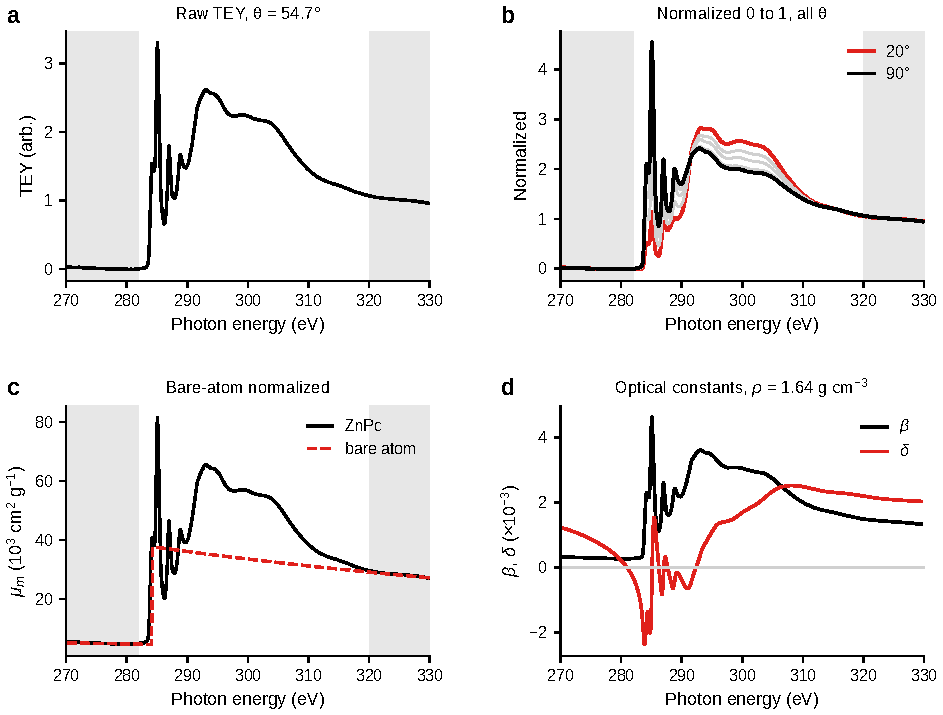
\includegraphics[width=\linewidth,height=0.75\textheight,keepaspectratio]{fig5-02_normalization}
  \caption[From raw signal to optical constants for the ZnPc dataset used in \cref{chap:znpc}.]{From raw signal to optical constants for the ZnPc dataset used in \cref{chap:znpc}. (a) Raw total electron yield at θ = \ang{54.7} with the pre-edge (270 to \qty{282}{eV}) and post-edge (320 to \qty{330}{eV}) windows shaded. (b) Zero-one normalization of every polarization geometry, from θ = \ang{20} (red) to \ang{90} (black), with each pre-edge mean set to 0 and one scale, the inverse median edge jump, shared by all geometries. (c) Mass absorption of the θ = \ang{54.7} spectrum after bare-atom normalization (black) against the bare-atom absorption of ZnPc (red, dashed). (d) Isotropic β from the mass absorption in c (black) and its Kramers-Kronig partner δ (red) at ρ = \qty{1.64}{g.cm^{-3}}.}
  \label{fig:6.2}
\end{figure}


\textbf{Normalization and NEXAFS channels.} \cref{fig:6.2} shows how X-ray Atlas derives optical constants from an uploaded measurement, here the ZnPc dataset used in \cref{chap:znpc} (accession 193bc0c5). The raw total electron yield (\cref{fig:6.2}a) carries the incident flux, the detector response, and the sample geometry in its absolute scale, so only its shape is meaningful. Two windows far from resonance, chosen by the contributor and here set to 270 to \qty{282}{eV} before the edge and 320 to \qty{330}{eV} after it, anchor every later step.\autocite{watts2006methods} The optical density channel subtracts the mean pre-edge signal of each geometry and divides every geometry by one shared scale, the inverse of the median edge jump (\cref{fig:6.2}b). The shared scale places the post-edge at unity to within the spread of edge jumps between geometries, 0.9 percent for this dataset, while preserving the relative dichroism. Because the scale is always positive, no trace is ever inverted. For ZnPc the \(\pi^{*}\) resonances near \qty{285}{eV} are strongest at \(\theta\) = \ang{90} and the \(\sigma^{*}\) band above \qty{290}{eV} at \(\theta\) = \ang{20}, the linear dichroism of the edge-on film analyzed in \cref{fig:2.8}. At \(\theta\) = \ang{54.7} the factor \(3\cos^{2}\theta - 1\) vanishes, and with it the dichroism of a uniaxial film\autocite{stohr2010nexafs}, so the spectrum at this angle supplies the isotropic response. The mass absorption channel places that spectrum on an absolute scale with a positive scale and an offset that match its window means to the bare-atom mass absorption of the molecular formula, computed from the Henke tables\autocite{henke1993x}, in the same two windows (\cref{fig:6.2}c). The imaginary index then follows as \(\beta = \lambda\rho\mu_{m}/(4\pi)\) for a stated density, here \(\rho\) = \qty{1.64}{g.cm^{-3}}, and \(\delta\) follows from the Kramers-Kronig transform of \(\beta\) embedded in the bare-atom \(\beta\) from \qty{10}{eV} to \qty{30}{keV},\autocite{watts2014calculation} as in \cref{fig:2.5}b (\cref{fig:6.2}d). Each channel is stored with the window choices that produced it, so a later change of window creates a new dataset revision (\cref{fig:6.4}).

In equation form, for the raw trace \(I_{g}(E)\) of geometry \(g\) with pre-edge mean \({\bar{I}}_{g}^{pre}\) and edge jump \(J_{g} = {\bar{I}}_{g}^{post} - {\bar{I}}_{g}^{pre}\), the optical density is \({OD}_{g}(E) = \left( I_{g}(E) - {\bar{I}}_{g}^{pre} \right)/\widetilde{J}\) with \(\widetilde{J} = {median}_{g}\, J_{g}\). The mass absorption is \(\mu_{m}(E) = a\, OD(E) + b\), with \(a > 0\) and \(b\) chosen so that the window means of \(\mu_{m}\) equal those of the bare-atom mass absorption \(\mu_{m}^{atom}(E)\) in the pre-edge and post-edge windows. The imaginary index is \(\beta(E) = \lambda\rho\mu_{m}(E)/(4\pi)\), with \(\delta(E)\) following from the Kramers-Kronig relation of \cref{chap:molecular-films}.

\textbf{Angle convention.} Angle-resolved NEXAFS can be reused only if the geometry of each trace is recorded without ambiguity, and published spectra report geometry variously as the X-ray incidence angle, the sample tilt, or the field angle, measured from either the surface or its normal. X-ray Atlas stores the orientation of the electric field itself (\cref{fig:6.3}). The polar angle \(\theta\) is measured from the sample normal \(\widehat{\mathbf{n}}\) to \(\mathbf{E}\), while the azimuth \(\phi\) is measured in the sample plane from the reference axis \(\widehat{\mathbf{x}}\) to the projection of \(\mathbf{E}\). This is the convention of \cref{fig:2.8} and \cref{chap:znpc}, in which \(\theta\) = \ang{90} places \(\mathbf{E}\) in the film plane, so the expressions of Stöhr used in \cref{chap:introduction}\autocite{stohr2010nexafs} apply to stored angles without conversion. Each trace keeps its ordered \((\theta,\phi)\) pair in the fields e\_field\_polar and e\_field\_azimuth, so geometries such as (\ang{90}, \ang{45}) and (\ang{45}, \ang{90}) remain distinct records, as they must for biaxial films in which the azimuth matters. Polar angles from −\ang{360} to \ang{360} are accepted so that laboratory motor angles can be entered directly, and when the angle columns are omitted, the trace takes a single fixed geometry set in the contribution form.

\textbf{Molecular identity resolution.} Chemical identity is resolved through InChI, SMILES, CAS number, and PubChem CID rather than through a free text name, since the same compound is commonly described by several shortened or trade names in the literature, particularly for newly engineered chemistries.Synonyms are stored against a single canonical molecule record and are searchable, so a contributor uploading under an unfamiliar name is still mapped to the correct underlying record. Molecules are further organized into hierarchical tags (for example, organic photovoltaic small molecule donor) that group chemically or functionally related compounds for browsing.

\begin{figure}
  \centering
  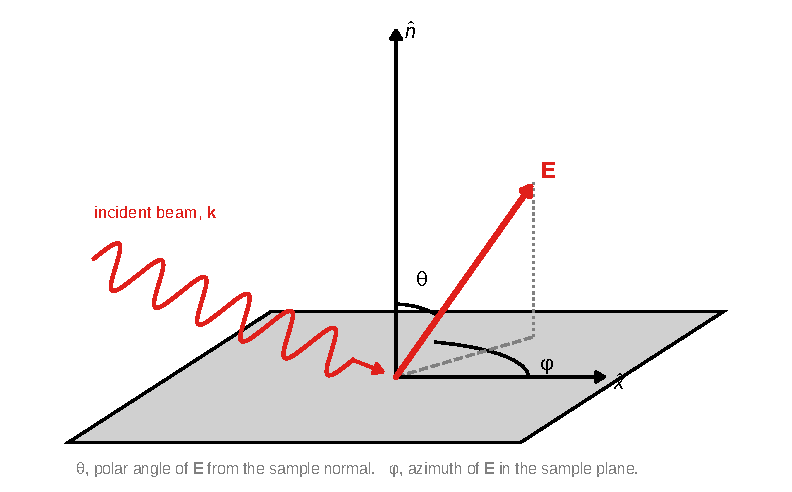
\includegraphics[width=\linewidth,height=0.75\textheight,keepaspectratio]{fig5-03_angle-convention}
  \caption[Polarization geometry stored with every trace.]{Polarization geometry stored with every trace. The incident wave (red) carries the electric field E, with θ the polar angle of E from the sample normal n̂ and φ its azimuth in the sample plane measured from x̂. Each trace keeps its ordered (θ, φ) pair, so geometries such as (\ang{90}, \ang{45}) and (\ang{45}, \ang{90}) remain distinct records.}
  \label{fig:6.3}
\end{figure}


\begin{figure}
  \centering
  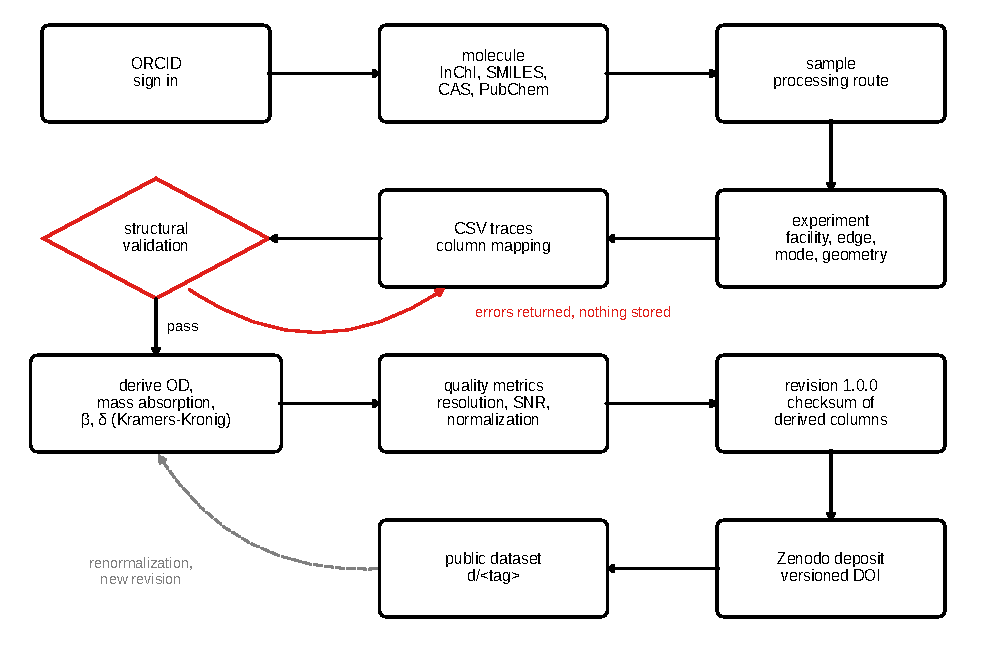
\includegraphics[width=\linewidth,height=0.75\textheight,keepaspectratio]{fig5-04_contribution-workflow}
  \caption[Contribution workflow for a new dataset.]{Contribution workflow for a new dataset. A contributor signs in with ORCID, resolves the molecule by InChI, SMILES, CAS number, or PubChem CID, describes the sample processing route and the experiment, and maps the columns of each uploaded CSV trace. Structural validation (red) returns errors and stores nothing for a malformed upload. Accepted uploads are converted to optical density, mass absorption, β, and δ, scored by the quality metrics, recorded as revision 1.0.0 with a checksum of the derived columns, deposited to Zenodo under a versioned DOI, and published. A later renormalization creates a new revision and a new Zenodo version (gray, dashed).}
  \label{fig:6.4}
\end{figure}


\textbf{Contribution workflow.} Each uploaded trace is a table of photon energy measurements. The contribution interface maps comma separated value (CSV) column headers, matched flexibly rather than requiring an exact header name, onto spectrum point rows, and requires photon energy to increase strictly monotonically within a trace. Angle resolved uploads are stored as separate traces per polarization geometry when the azimuthal and polar angle columns vary across the upload, or as a single fixed geometry set in the contribution form when those columns are omitted. Raw absorption, optical density, mass absorption, and the real and imaginary parts of the index of refraction are persisted at ingestion or recalculation, each with an optional uncertainty column; quantities that are trivially derived from these in the browser, such as the imaginary part of the atomic scattering factor, are computed on demand and never written back to the database.

\Cref{fig:6.4} follows a dataset from sign-in to publication, with each stage collecting one record type of the data model in \cref{fig:6.1} in the order in which later stages depend on it. The contributor authenticates through ORCID, so attribution attaches to a persistent identity from the start, then resolves the molecule by a structural identifier rather than a name, describes the sample processing route and the experiment (facility, absorption edge, detection mode, and geometry), and maps the columns of each uploaded trace. Structural validation is the single gate between the contributor and the database. A trace with non-monotonic energies, missing metadata, or inconsistent geometry labels is returned with its errors and nothing is stored, so an incomplete record never becomes visible to other users. A trace that passes is converted into the channels of \cref{fig:6.2}, scored by the quality metrics described under Technical Validation, and recorded as revision 1.0.0 together with a checksum of its derived columns. The revision is deposited to Zenodo under a versioned DOI before the dataset becomes public, so every public dataset is citable from its first appearance. The raw signal is immutable from this point, but the processing is not. A change that alters a derived quantity, such as a new normalization window, returns the dataset to the derivation step and produces a new revision and a new Zenodo version under the same concept DOI (\cref{fig:6.4}, dashed).

\textbf{Versioning and data deposition.} The underlying raw experimental signals are immutable; however, processing choices such as normalization windows, peak assignments, and similar processing choices are routinely refined after the initial upload. Only a change that alters a derived numerical quantity (\(\beta(E),\delta(E),\ f_{1}(E),\ \).etc) increments the dataset's major, minor, or patch version; contributor and attribution changes do not. Every version increment is recorded as an immutable revision carrying the kind of change (an initial upload, a normalization change, a Kramers-Kronig calculation or recalculation, or an auxiliary file addition or removal) and a checksum of the derived columns, so a specific configuration can always be recovered. Each version increment is mirrored automatically as a new version deposited to Zenodo under the dataset's concept DOI, giving every dataset a persistent, versioned citation independent of the X-ray Atlas web application's own availability.

\textbf{Attribution.} Contributors authenticate through their ORCID iD, with a dataset's contributor list built from that identity rather than a free text author field. A contributor is recorded with a role (collection, processing, or curation) and a claim status, so a collaborator can be added to a dataset by a colleague and later confirm or decline that attribution themselves. Larger beamtime collaborations can be recorded as an attribution team with a principal investigator, an experiment lead, and a member list, so a single collection run that produced many datasets does not require re-entering the same contributor list on every upload. A further, optional layer lets users construct versioned, independently authored optical models (peak assignments and optical tensors fit to one or more raw datasets), each signed off by its listed authors and citable on its own, separate but trackable back to the original experimental measurement.

\textbf{Authentication.} Reading public data requires no account. Contributors sign in through ORCID, so every record they create is tied to a persistent researcher identity. Passkeys provide passwordless sign-in. Actions that cannot be undone or that change ownership, such as merging or deleting datasets and issuing a command-line credential, additionally require a passkey confirmation within the preceding two hours. Administrator actions require a higher assurance level still. Command-line credentials carry read or write scope, are attached only to the host that issued them, and can be revoked by their owner.

\section{Data Records}\label{sec:data-records}

\Cref{tab:6.1} lists the fields of the two record types most users of the database will query directly, the experiment (dataset) record and its spectrum points, alongside their units and source. X-ray Atlas currently hosts 13 molecules, 47 experiments, and 132,419 spectrum points, contributed by 12 registered users across 3 facilities. Data are stored and served from a hosted relational database (PostgreSQL) and are additionally deposited to Zenodo on every version increment, so a dataset remains citable and retrievable independent of the X-ray Atlas application's own uptime. Contributed datasets are licensed under CC BY 4.0; the application code that serves them is licensed separately under the MIT license.

\begin{longtable}[]{@{}
  >{\raggedright\arraybackslash}p{(\linewidth - 4\tabcolsep) * \real{0.2297}}
  >{\raggedright\arraybackslash}p{(\linewidth - 4\tabcolsep) * \real{0.5552}}
  >{\raggedright\arraybackslash}p{(\linewidth - 4\tabcolsep) * \real{0.2151}}@{}}
\caption{Core fields of the experiment and spectrum point records. The production schema stores several of these as separate, normalized tables; this table lists the field as it is queried, not its physical storage location.}\label{tab:6.1}\tabularnewline
\toprule\noalign{}
\begin{minipage}[b]{\linewidth}\raggedright
\textbf{Field}
\end{minipage} & \begin{minipage}[b]{\linewidth}\raggedright
\textbf{Description}
\end{minipage} & \begin{minipage}[b]{\linewidth}\raggedright
\textbf{Source}
\end{minipage} \\
\midrule\noalign{}
\endfirsthead
\toprule\noalign{}
\begin{minipage}[b]{\linewidth}\raggedright
\textbf{Field}
\end{minipage} & \begin{minipage}[b]{\linewidth}\raggedright
\textbf{Description}
\end{minipage} & \begin{minipage}[b]{\linewidth}\raggedright
\textbf{Source}
\end{minipage} \\
\midrule\noalign{}
\endhead
\bottomrule\noalign{}
\endlastfoot
\begin{minipage}[t]{\linewidth}\raggedright
Photon energy\\
(eV)\strut
\end{minipage} & Incident photon energy of the measurement & contributor upload \\
Raw absorption (arb.) & Raw measured absorption, including incident beam intensity, and measurement uncertainties. & contributor upload \\
\begin{minipage}[t]{\linewidth}\raggedright
Optical density\\
(arb.)\strut
\end{minipage} & Normalized absorption, with propagated uncertainty & derived at ingestion \\
\begin{minipage}[t]{\linewidth}\raggedright
Mass absorption\\
(cm\textsuperscript{2}/g)\strut
\end{minipage} & Bare atom normalized mass absorption computed from the optical density, with propagated uncertainty & derived at ingestion \\
Index of refraction, \(\beta(E)\) & Imaginary part of the index of refraction, with propagated uncertainty & derived at ingestion \\
Index of refraction, \(\delta(E)\) & Kramers-Kronig transform of beta, with propagated uncertainty & derived at ingestion \\
Polarization geometry \(({^\circ})\) & Sample and polarization orientation for the trace & contributor upload \\
Absorption edge & Target atom and core level (K, L1 to L3, M1 to M3) & contributor upload \\
Detection mode & Total electron yield, partial electron yield, fluorescence yield, or transmission & contributor upload \\
Facility and instrument & Collection facility, beamline, and instrument status & contributor upload \\
Sample processing route & Deposition method, solvent, substrate, patterning layer, nominal thickness, vendor & contributor upload \\
\begin{minipage}[t]{\linewidth}\raggedright
Dataset version\\
(major.minor.patch)\strut
\end{minipage} & Version of this dataset's processing and derived values & generated \\
Zenodo DOI & Persistent, versioned citation for this dataset version & generated at publish \\
Contributor ORCID and role & Identity and role of each person credited on the dataset & contributor upload \\
Linked publication DOI & Source or citing publication associated with the dataset & contributor upload \\
\end{longtable}



\begin{figure}
  \centering
  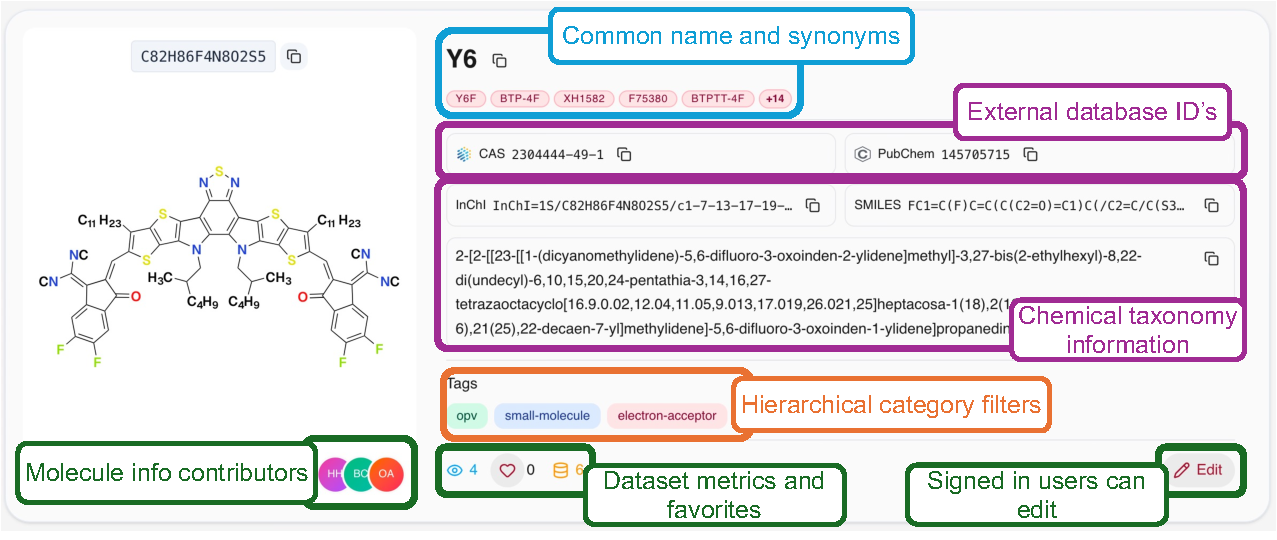
\includegraphics[width=0.85\linewidth,height=0.75\textheight,keepaspectratio]{fig6-05_molecule-record}
  \caption[X-ray Atlas molecule record UI.]{X-ray Atlas molecule record UI. Molecules are linked to external CAS and PubChem registries, and taxonomical information is stored. Molecule synonyms provide a searchable many to one representation to serve the wide community with multiple names of the same molecule. Tags provide hierarchical groupings of common or similar molecules. Users can contribute edit or modify records, as well as favorite records to make them easier to return to.}
  \label{fig:6.5}
\end{figure}


\section{Technical Validation}\label{sec:technical-validation}

Three independent checks apply to a contributed dataset, operating at different points in its life to capture different errors.

\textbf{Structural validation at upload}. At the time of upload the datasets are validated against the schema with type checking enforced. Datasets must have monotonic photon energies for each polarization geometry, experimental metadata (facility, instrument, and edge) and consistent geometry labeling for angle resolved uploads. These faults are recorded during upload preventing malformed or incomplete data from entering the database.

\textbf{Automated quality metrics.} Once ingested, a dataset is scored against quantitative quality metrics computed from the data itself. Three sub-scores, each mapped onto 0 to 100 by fixed monotone breakpoints, are computed for every dataset. Energy sampling is scored from the median spacing between adjacent energies, from 100 at \qty{0.028}{eV} or finer down to 8 beyond \qty{0.52}{eV}. Signal to noise is scored from the ratio of the mean absolute signal to its standard deviation over the populated samples, from 14 below a ratio of 2.2 to 100 above 40. Normalization quality is scored from the pooled mean absolute deviation of the optical density from 0 in the pre-edge window and from 1 in the post-edge window, from 100 at0.012 or less down to 6 beyond 0.32. The dataset score is the mean of the available sub-scores and is reported in four tiers, excellent at 86 or above, good from 66, fair from 38, and poor below 38.

\begin{figure}
  \centering
  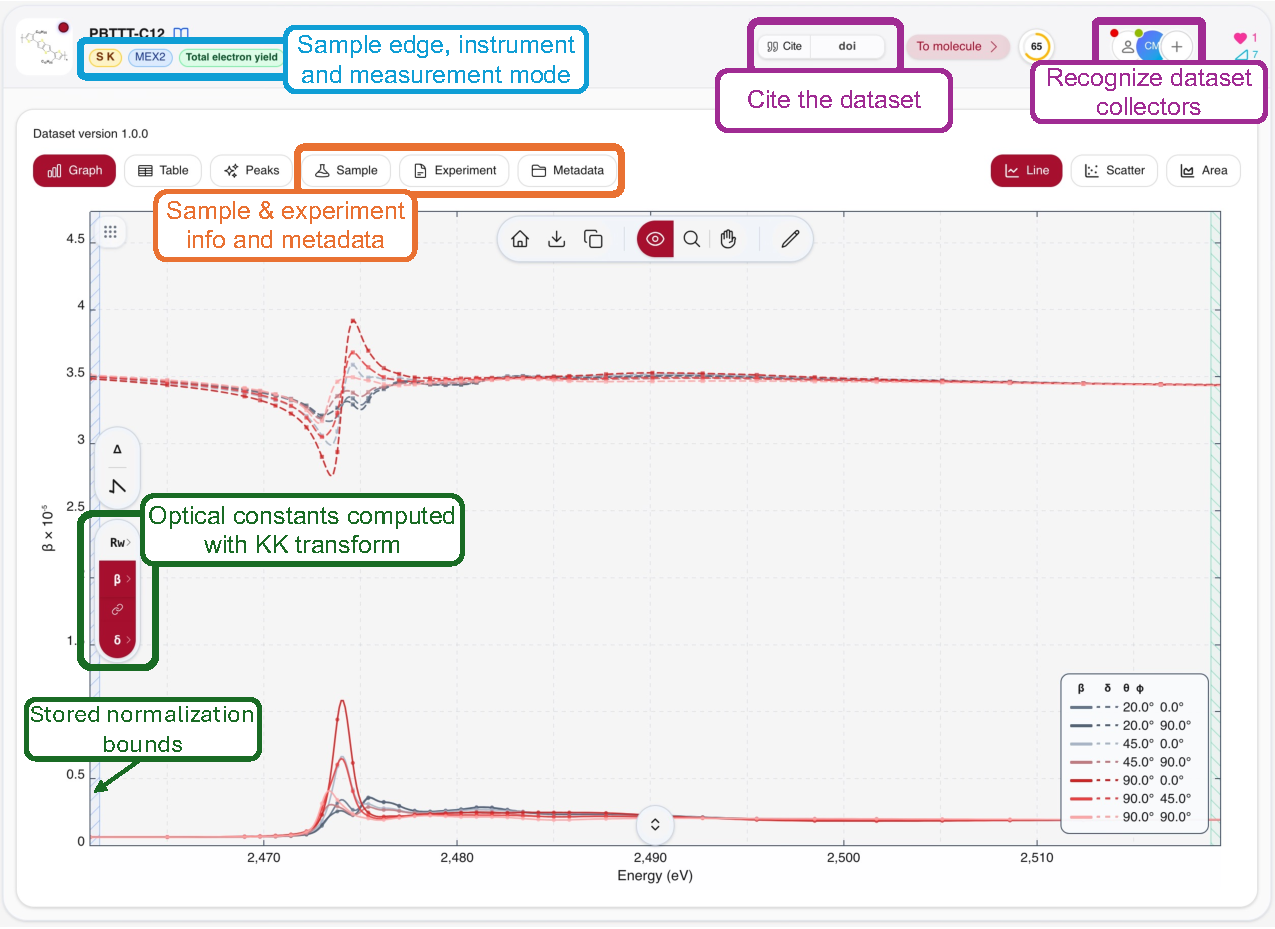
\includegraphics[width=0.85\linewidth,height=0.75\textheight,keepaspectratio]{fig6-06_dataset-record}
  \caption[X-ray Atlas NEXAFS Dataset UI.]{X-ray Atlas NEXAFS Dataset UI. Datasets store the full processing specifications to convert the raw measured signals into optical constants.}
  \label{fig:6.6}
\end{figure}


\textbf{Peer review and publication cross reference.} Cross referencing data stored in the database against either an original publication or a new publication featuring it provides additional confidence that the data quality meets the standards of peer review. This added confidence implies that sample preparation follows a usual approach, and data collection and analysis follows from the standards for a given facility and instrumentation, while providing a direct reference back to the original manuscript bearing more detailed methods and conclusions regarding the data.

\section{Usage Notes}\label{sec:usage-notes}

\begin{figure}[htp]
  \centering
  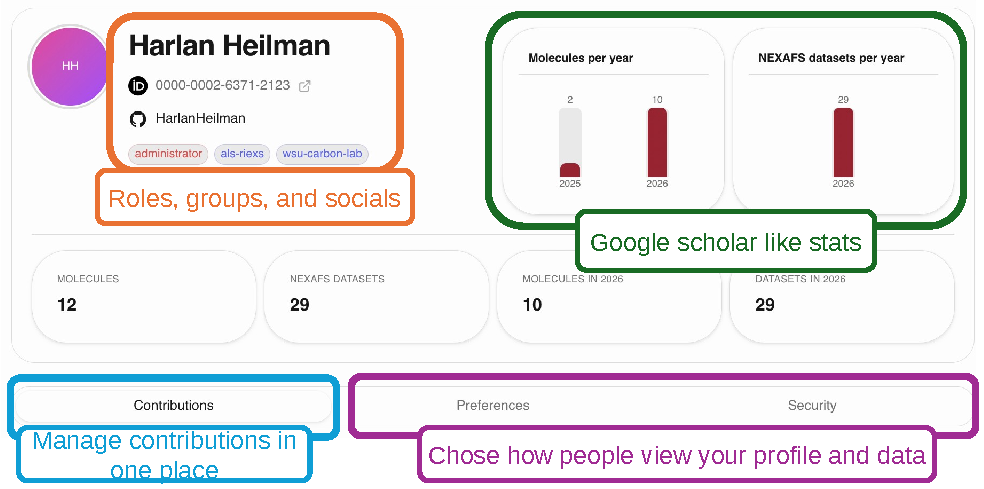
\includegraphics[width=\linewidth,height=0.75\textheight,keepaspectratio]{fig6-07_user-profile}
  \caption[X-ray Atlas User profile.]{X-ray Atlas User profile. Minimal user information is stored only enough to ensure connection and authentication though ORCID. Users can choose to create research groups and link other socials if they wish to. Contribution metrics are stored with similar calculation as though Google Scholar and similar sites. Users have full autonomy to edit how or if they appear to the rest of the community as well as maintain edit and remove data they contribute.}
  \label{fig:6.7}
\end{figure}

The web interface at \pkg{xrayatlas}.wsu.edu supports browsing and searching by molecule, facility, edge, or tag and shows each dataset's quality metrics alongside its trace. Beyond the browser, X-ray Atlas data is built to be addressed programmatically. A python package, distributed as \pkg{xrayatlas} on the Python Package Index, exposes the same molecule, datasets and optical model records available through the website to scripted analysis, letting a researcher pull a dataset directly into a notebook or an analysis pipeline rather than downloading files by hand. A companion command line interface (CLI), shipped as a single compiled binary in the manner of tools such as the Hugging Face CLI, gives the same access from the terminal for scripting and automation. This programmatic layer is deliberate, framing the registry alongside platforms such as Hugging Face and Weights and Biases rather than as a bespoke scientific database, so that an analysis agent or training pipeline can discover and pull a relevant NEXAFS dataset the same way it would pull a pretrained model, with provenance and attribution carried along automatically rather than left for the user to reconstruct.



Citation follows two conventions depending on scope. An individual dataset is cited by its own versioned DOI, in the form of the dataset name and DOI, adapted from the original publication, hosted by X-ray Atlas; the entire collection is cited by a collection level DOI together with the date accessed.

\section{Programmatic Access}\label{sec:programmatic-access}

\begin{figure}[htp]
  \centering
  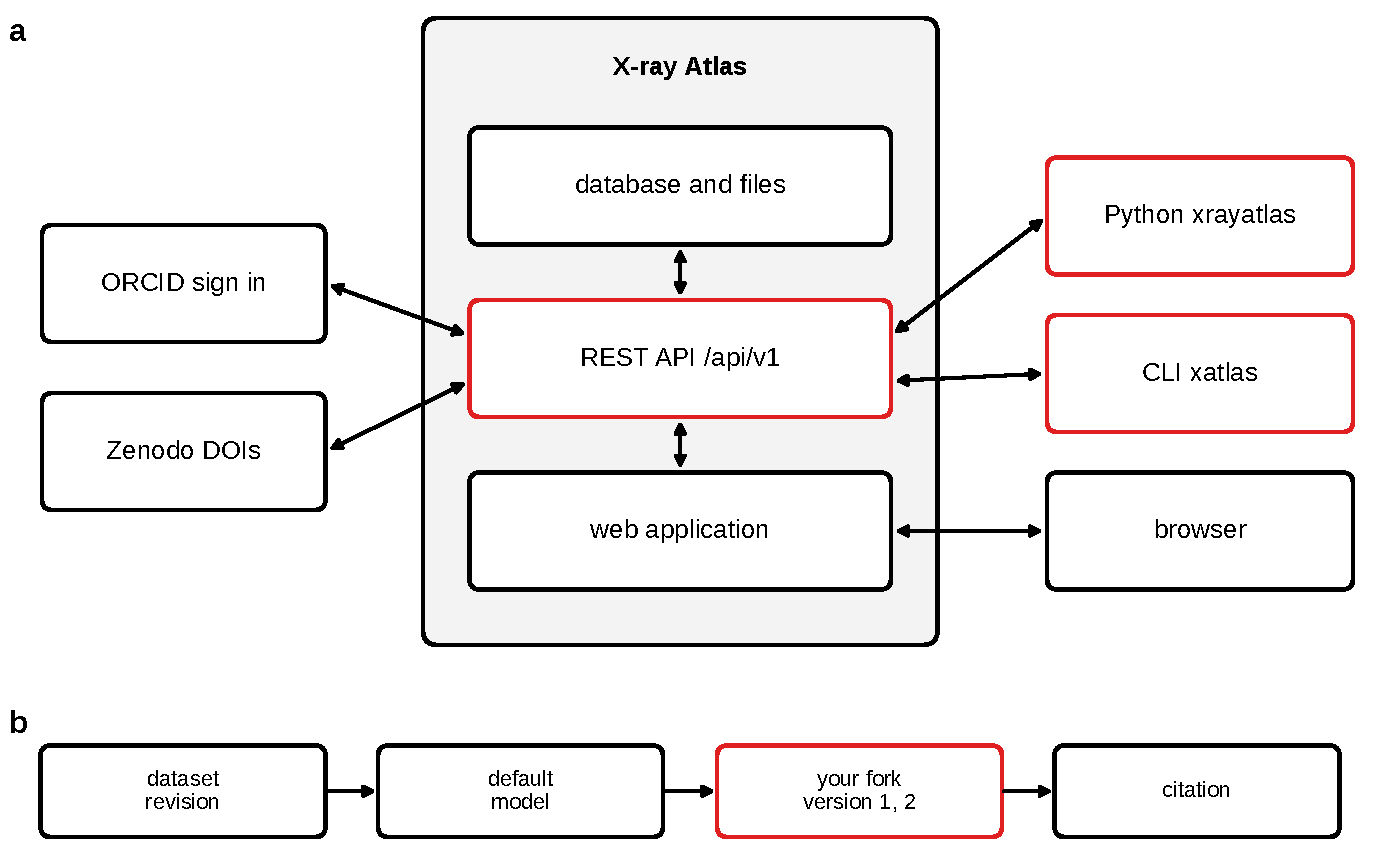
\includegraphics[width=\linewidth,height=0.75\textheight,keepaspectratio]{fig6-08_architecture}
  \caption[Architecture of X-ray Atlas and the lineage of optical models.]{Architecture of X-ray Atlas and the lineage of optical models. (a) X-ray Atlas holds the database and files behind the web application and the REST interface /api/v1, with ORCID handling sign-in and Zenodo issuing DOIs. The browser reaches the web application, while the \pkg{xrayatlas} Python package and the \pkg{xatlas} command-line client (red) share the REST interface. (b) An optical model pins a dataset revision, the default model can be forked into independently versioned models (red), and a citation lists the model, its dataset revisions, and every ancestor in the chain.}
  \label{fig:6.8}
\end{figure}



The programmatic layer described above rests on the architecture in \cref{fig:6.8}a. A single store of records and files sits behind two interfaces. The web application serves people through the browser, and the REST interface /api/v1 serves programs, shared by the \pkg{xrayatlas} Python package and the \pkg{xatlas} command-line client so that a script and a terminal session see the same records under the same permissions. Identity and persistence are delegated to external services, ORCID for sign-in and attribution and Zenodo for versioned DOIs, so neither depends on the availability of X-ray Atlas itself. The client never fits peaks, computes optical constants, or normalizes spectra. Normalization is computed by the server, so every client receives the same derived channels. Optical models extend the same versioning from data to analysis (\cref{fig:6.8}b). A model, a set of peak assignments with \(\delta\) and \(\beta\) for each tensor component on a shared energy axis, fit by its authors to one or more datasets in the manner of \cref{chap:resonances} and of the bond-traceable tensors of Murcia et al.\autocite{murcia2026quantitative}, pins the exact dataset revisions it was built from. The default model for a dataset can be forked, with each fork versioned and authored independently while keeping a link to its parent. A citation of any model lists the model, the dataset revisions it pins, and every ancestor in its chain, so credit reaches each contributor to the measurement, the processing, and the analysis. Likewise, a result built on a model can be traced back to the raw spectra behind it. The \pkg{xrayatlas} package is released on PyPI and remains under active development.

The package requires Python 3.10 or newer and installs with \code{pip install xrayatlas} or \code{uv add xrayatlas}. Authentication is shared with the command-line client, so a single \code{xatlas login} writes the credential that both read. The listing below pulls the ZnPc dataset of \cref{chap:znpc}, publishes an optical model built on it, forks and compares that model, and pins the session to the exact revisions it used. The \pkg{xatlas} client exposes the same operations from the terminal. \code{xatlas search}, \code{xatlas molecules}, and \code{xatlas datasets} find and fetch records, \code{xatlas upload} contributes a dataset through the validation of \cref{fig:6.4}, \code{xatlas models} reads, pushes, and publishes optical models, and \code{xatlas lock} and \code{xatlas restore} write and replay the same lockfile as the Python client, so an analysis recorded in one can be reproduced in the other.

\textbf{Query the database}. Using the CLI it is possible to directly query the database, applying filters and identifying the datasets that are useful or interesting. Once found these datasets can be stored locally in tabular forms such as CSV files, parquet files, or as local SQLite snapshots.

\begin{codeblock}
# Browse the catalog by molecule, edge, and facility
xatlas molecules tree phthalocyanine
xatlas molecules tree --group edge,molecule,facility

# Read-only SQL on the public spectrum_points relation
xatlas query "SELECT atlas_dataset_id, molecule_id, facility_name, COUNT(*) AS n_points
              FROM spectrum_points
              WHERE edge_label = 'C(K)' AND facility_name ILIKE '%light source%'
              GROUP BY atlas_dataset_id, molecule_id, facility_name
              ORDER BY n_points DESC"

# The same SQL on a local SQLite snapshot
xatlas datasets fetch d/193bc0c5 --out ./data --format sqlite
xatlas query --db ./data/spectra.sqlite \
    "SELECT DISTINCT theta_deg, phi_deg FROM spectrum_points ORDER BY theta_deg"
\end{codeblock}

The same queries are available in Python, where lightweight dataset summaries can be searched by molecule, edge, DOI, or Atlas identifier without downloading any spectra, and a local snapshot can be queried directly with standard tools such as \pkg{pandas}.

\begin{codeblock}
import sqlite3

import pandas as pd
import xrayatlas as xa

# Lightweight summaries filtered by molecule, edge, DOI, or Atlas id; no spectra are downloaded
for summary in xa.datasets.search(molecule_id=molecule_id):   # UUID from the SQL above
    print(summary.atlas_dataset_id, summary.edge_label,
          summary.spectrum_point_count, summary.dataset_doi)

# Query the local snapshot directly with pandas
with sqlite3.connect("data/spectra.sqlite") as con:
    iso = pd.read_sql(
        "SELECT energy_ev, mass_absorption, beta FROM spectrum_points "
        "WHERE abs(theta_deg - 54.7) < 0.1 ORDER BY energy_ev",
        con,
    )
\end{codeblock}

\textbf{Accessing datasets}. Once a dataset is identified it can be pulled into a coding environment such as Python using the \pkg{xrayatlas} package. From there metadata information such as versions, molecule information, publication information and more can be accessed, along with the spectral data including both the raw uploaded data and the derived quantities such as optical constants.

\begin{codeblock}
import xrayatlas as xa

ds = xa.datasets.get("d/193bc0c5")               # current version, cached by version
pinned = xa.datasets.get("d/193bc0c5", "1.0.0")  # pinned version

print(ds.molecule_name, ds.edge, ds.facility, ds.instrument, ds.version)
print(ds.publication_dois)

spec = ds.spectra()           # energy_ev, theta_deg, phi_deg, raw_abs, i0,
                              # od, mass_absorption, beta, delta
raw = ds.spectra(raw=True)    # uploaded signal and I0 only
geometries = ds.geometries()  # ordered (theta_deg, phi_deg) pairs; (90, 45) != (45, 90)

# One trace per geometry, and the isotropic (magic-angle) spectrum
traces = {geom: trace for geom, trace in spec.groupby(["theta_deg", "phi_deg"])}
iso = spec[(spec.theta_deg - 54.7).abs() < 0.1]

ds.aux_files.download("aux/", kind="sample")     # sample-aux/ files from the dataset bundle
models = ds.models(scope="public")               # optical models that link this dataset
with open("znpc.bib", "w") as f:
    f.write(ds.bibtex())
\end{codeblock}

\textbf{Working with datasets}. The package makes available tools to directly interact with a dataset, including modifying normalization schemes and peak assignments, before pushing to the remote database. Normalization windows can be set once for every channel or separately for the optical density, the mass absorption, and β, and peak assignments from an independent fit are validated row by row before upload. A change to the normalization of a dataset creates a new revision and a new Zenodo version, so earlier analyses that pinned the previous version remain reproducible.

\begin{codeblock}
import pandas as pd
import xrayatlas as xa

# One pre-edge and post-edge window pair for every channel
norm = xa.Normalization(pre=(270.0, 282.0), post=(320.0, 330.0))

# Or a separate pair for each channel
norm_pc = xa.Normalization(
    scope="per_channel",
    od=xa.WindowPair(pre=(270.0, 282.0), post=(320.0, 330.0)),
    massabsorption=xa.WindowPair(pre=(270.0, 282.0), post=(320.0, 330.0)),
    beta=xa.WindowPair(pre=(270.0, 282.0), post=(320.0, 330.0)),
)

# Peak assignments from your own fit; unrecognized columns are stored as each peak's params
peaks = pd.DataFrame({
    "center_ev":  [284.2, 285.1, 287.1, 288.9],
    "kind":       ["pi-star", "pi-star", "other", "other"],
    "transition": ["C2 1s -> MO 117", "C3 1s -> MO 119",
                   "C2 1s -> MO 124", "C1 1s -> MO 124"],
    "amplitude":  amplitudes,          # arrays of length 4 from the fit
    "width":      widths,
    "fit_tool":   "refloxide",
})
checked = xa.validate_peaks(peaks)  # ValidationError names the offending row and column
\end{codeblock}

\begin{codeblock}
# Change the dataset's own normalization (a new revision and a new Zenodo version)
xatlas datasets push d/193bc0c5 --normalization norm.json --dry-run
xatlas datasets status d/193bc0c5
\end{codeblock}

\textbf{Uploading datasets and optical models}. The Python package and the command-line client both provide handles for uploading new datasets and new optical models into the database. An upload requires a credential with write scope and can first be run as a dry run, which applies the same structural validation as a real upload without writing anything. The file name of a contributed spectrum encodes its edge, detection mode, and beamline, so that these fields are set consistently at ingestion.

\begin{codeblock}
# A credential with write scope, then a dry run of the upload
xatlas auth login --write --name "lab laptop"
xatlas upload C-K_TEY_ALS_5.3.2_lab_vendor.csv --molecule "zinc phthalocyanine" \
    --process-method dry --dry-run       # six-token name sets edge, mode, and beamline

# Pull a published model to disk
xatlas models pull k7m2xq4n --out ./znpc-model
\end{codeblock}

With a dataset uploaded, new optical models can be defined by modifying the normalization scheme and the method by which the optical tensor is derived. Building a model forks the default model of the dataset, attaches a normalization, peak assignments, and a tensor in the molecular or film frame, and publishes an immutable version with its own citation. A published model can itself be forked and refined, for instance with peak parameters refined against reflectivity, and the lineage of every version travels with its citation together with the dataset revisions it pins. A lock file records every dataset and model revision used in an analysis so that the session can be replayed later.

\begin{codeblock}
import numpy as np
import xrayatlas as xa

ds = xa.datasets.get("d/193bc0c5")

# Complex payload with delta in the real part and beta in the imaginary part, (n_energy, 2)
values = np.stack([delta_xx + 1j * beta_xx, delta_zz + 1j * beta_zz], axis=1)

with xa.model(datasets=[ds], title="ZnPc ML-DFT tensor") as builder:  # forks the default model
    builder.normalization = norm
    builder.peaks = peaks
    builder.tensor = xa.Tensor.from_array(values, energy_ev=energy, components=["xx", "zz"],
                                          frame="molecular", units="1")
model = builder.publish()             # explicit and never retried; versions are immutable

model.set_visibility("public")        # private, shared, or public
channels = model.normalized(ds)       # server-computed od, mass_absorption, beta
print(model.cite())                   # BibTeX of this published version

# Fork, publish the next version, and compare the two
with model.fork(title="ZnPc ML-DFT tensor, reflectivity refined") as fork:
    fork.peaks = refined_peaks
refined = fork.publish()
aligned = xa.compare([model, refined], tolerance_ev=0.2).peaks
lineage = refined.lineage()           # visible ancestors, newest first

# Pin every dataset and model revision used in this session, and replay it later
xa.lock("analysis.lock")
xa.restore("analysis.lock")
\end{codeblock}

\section{Code Availability}\label{sec:code-availability}

The X-ray Atlas web application, database schema, Python package, and command line client are developed in the open at github.com/WSU-Carbon-Lab/xray-atlas. Application code is licensed under the MIT license; contributed datasets are licensed separately under CC BY 4.0.

\chapter{Conclusion \& Outlook}\label{chap:conclusion}

Resonant soft X-ray scattering has for two decades distinguished the components of organic materials by tuning photon energy across an absorption edge, yet the information it returns about buried molecular states has been bounded by how the optical response is described. This dissertation set out to show that polarized resonant measurements of molecular films already contain more information about those states than prior analyses recover, with the limit lying in the optical model used to interpret them rather than in the measurement. Reflectivity studies of molecular films have obtained that model in one of two ways, tabulating the tensor from NEXAFS of a reference film and holding it fixed at every depth, or fitting it freely at each measured energy. One question was asked of each practice. The first concerned what becomes measurable once the tabulated tensor is replaced by one derived from the electronic transitions of the molecule, and the second concerned how the physical constraints that make such a derivation possible can be carried into the recovery of a tensor that no reference supplies. The approach throughout has been to build the optical tensor from the electronic transitions that produce it, so that each parameter of a fit corresponds to a physical property of the molecule or of its arrangement in the film. Under the first question the tensor was reduced to molecular orientation and density, and under the second the individual resonances themselves were allowed to vary with depth.

For the first question, the ML-refined DFT tensor was built into the analysis of polarized resonant reflectivity from vapor-deposited ZnPc films on native-oxide silicon, with each layer described by a molecular tilt and a density alone. With the spectral shape fixed by the molecule, these few structural parameters must account for the reflectivity at every energy and in both polarizations, and the amplitudes and phases of the fringes across the edge become a joint constraint on them. Across the pre-edge and the resonance series the resulting model described the data as well as or better than free optical constants, from an order of magnitude fewer parameters and with correspondingly smaller uncertainties. Measurements that had been treated as a set of independent energies thereby became a single, overdetermined measurement of molecular state. In a Fisher sensitivity analysis, the constraint on the sub-monolayer interfacial features was traced to the ML-DFT tensor, through the coupling it imposes on fringe amplitude and phase across energy and polarization, and the profile of a second film grown under identical conditions to a different thickness agrees with the first. The first hypothesis therefore holds for ZnPc on silicon, with reflectivity measurements of the kind already in hand fixing the order and density of the interfacial layers, within the assumed depth profile, with uncertainties below the real-space length set by the largest momentum transfer measured.

What an energy-by-energy fit permits became plain in the same comparison. Nothing in such a fit ties the optical constants found at one energy to those found at another. It can return dichroism that no arrangement of the molecule produces, and dispersion inconsistent with the absorption at other energies, a violation of causality that cannot be detected short of sampling the whole edge. In the free fit of ZnPc the surface and buried layers took optical constants that were extreme and poorly determined, including an off-scale dichroism near \qty{287}{eV}, and their low-energy trends broke at the diagnostic energy, leaving the orientation read from them dependent on which energy was analyzed. The ML-DFT tensor is causal and symmetric by construction. Because it admits only ZnPc, the customary assignment of interfacial layers to contamination or oxidation also became testable, since a foreign species at an interface would appear as misfit at the molecule's own resonances. The resonance series of those layers was reproduced with a different tilt and density. Contamination and oxidation are not required by the data within the sensitivity of that series, and the interfacial layers are the molecule itself in other packing and orientational states.

How a wrong tensor behaves in a fit could not be reasoned out in advance, and both of the anticipated behaviors appeared. The largest misfit of the ML-DFT slab model, a phase shift of the s-polarized fringes at the diagnostic energy, was localized to that energy and traced to the structure, since replacing the slabs with the continuous gradient profile removed it with the optical model unchanged. When the same films were fit with a tensor held to the NEXAFS of the reference film, the fit matched the data at the three lower resonant energies and failed at the two energies of strongest orientation sensitivity, placing the misfit where the signature of the error was largest. In Alq\textsubscript{3} a borrowed NEXAFS spectrum misfit every measured energy by a similar factor and was partly absorbed into the structure, with the substrate density driven to a value that the stoichiometry and packing of the molecule cannot allow. We surmise that the difference lies in whether a structural parameter can mimic the error. A change in absorption common to every resonance resembles a density gradient at a fixed spectral shape. Its error spreads across all energies and is partly taken up by the density, whereas an error confined to particular transitions has no structural counterpart and remains as misfit at the energies where those transitions dominate. Only errors of the second kind therefore appear in the residuals of a fixed tensor. Errors of the first kind surface as structural parameters that violate independent constraints, as the Alq\textsubscript{3} density did, and are corrected only when the strengths of individual resonances are free to depart from the reference, the step taken under the second question.

The depth profile returned by this analysis is a product of the first question. At the oxide interface the molecules adopt a lower-density state oriented closer to face-on, and at the free surface a denser state oriented near the magic angle, and each relaxes into the edge-on bulk over roughly one molecular layer. The interfacial state occupies less than a monolayer of a thin film, below the scale that any fit with free optical constants could resolve. Substrate patterning predicts that the first molecular layer already carries the bulk orientation, a prediction inconsistent with a face-on interfacial state beneath an edge-on bulk. The profiles are instead consistent with a growth picture in which substrate adhesion, which favors face-on molecules, competes with π-π cohesion, which favors edge-on packing, so that the gradient records the crossover from interface-dominated to bulk-dominated growth. One consequence is that films grown to partial coverage capture a transient state of the growth front and need not represent the buried interface of a continuously deposited film. These conclusions concern one molecule on one substrate, and the interfacial state on patterning underlayers such as CuI and graphene, where the bulk texture is face-on, can now be measured in the same way.

For the second question, the optical response was written as a sum of Kramers-Kronig consistent oscillator pairs, each a Gaussian absorption with its Dawson-function conjugate tied to an ML-DFT transition cluster and carrying a transition energy, a width, an oscillator strength, and a dipole orientation. Every trial spectrum in a fit is then causal, the tensor follows from the dipoles, and the parameter count is set by the number of transitions in the molecule, where the Kramers-Kronig consistent bases of Kuzmenko and of Stone et al. gain a basis function with every energy measured. With this basis, the amplitudes of individual resonances were refined as functions of depth together with the film structure in both Alq\textsubscript{3} and ZnPc, which satisfies the first part of the second hypothesis. In Alq\textsubscript{3} the degeneracy between the optical model and the film density was removed, the substrate density was no longer driven to an unphysical value, and the misfit fell at every measured energy. The absorption rises toward the substrate across all of the refined resonances, with the third nearly suppressed at the free surface before growing into the bulk and toward the interface. The cause of that evolution cannot yet be assigned. Hydrocarbon contamination at the surface, with the suppressed resonance then an artifact of the model, conformational changes that alter the transition rates near each interface, and hybridization driven by the interfacial potentials all remain consistent with the data, because the optical constants away from the measured energies are inferred from the dispersion of each oscillator.

In the ZnPc films the amplitude of each of the four principal resonances was refined with depth and its dipole cone angle refined once for the whole film, with the tilt and density held at the profile of the first question. The two lowest π* resonances, assigned in the ML-DFT clusters to excitation of two benzo-ring carbon sites into the lowest and a higher unoccupied orbital, exchange oscillator strength between the two interfaces. The first weakens at the free surface and strengthens at the oxide while the second does the reverse, with their summed strength close to the reference value at both boundaries. The third resonance weakens at the oxide interface, the fourth, assigned to the pyrrole carbon bound to nitrogen, strengthens most in relative terms at the oxide where the π* manifold meets the σ* onset, and the cone angles of the π* resonances stay close to the ring normal. These changes differ from one transition to the next, and no rescaling of the reference spectrum reproduces them. The second hypothesis therefore holds for the strengths of individual resonances. We surmise that the exchange between the two lowest resonances is a redistribution of spectral weight between the lowest unoccupied states as the local packing changes. Three mechanisms remain, each with its own signature. Hybridization or charge transfer at the oxide would confine the change to the first molecular layers and shift the transition energies as well as the strengths. Packing-dependent π overlap would make the ratio of the two strengths follow the local tilt wherever the same tilt recurs. Disorder at the free surface would broaden every resonance and lower its anisotropy without exchanging weight between two. Separating them requires a refit with the cone angle of each resonance free at the surface, in the bulk, and at the interface, together with a fixed-angle scan across the edge dense enough to constrain it. Until that measurement is made, the depth dependence of dipole orientation remains open.

The ambiguity in Alq\textsubscript{3} traces to the measurement as much as to the model. Because δ at each energy depends through the Kramers-Kronig relations on β at every other energy, optical constants known exactly at a few energies leave the spectrum between them undetermined, and a handful of energies supplies fewer observables than there are transition parameters to constrain. In synthetic spectra of a known carbon edge, part of the spectrum was recovered with energies placed on the resonances or chosen by a Gaussian-process design, the recovered fraction was essentially unchanged by a tenfold gain in precision at those energies, and the spectrum was constrained far better by a continuous scan across the edge with larger noise at each point than by any sparse set. For sparse measurements the number and placement of energies set the limit before the precision at any one of them does, and the sampling claim of the second hypothesis holds as well. Continuous energy scans should therefore anchor future resonant reflectivity, with the same sampling framework used to choose any additional energies before a beamtime and the oscillator construction serving as a generator of causal optical constants for planning measurements and for training learned inversions.

Two further parts of the second question remain open. The limit in which no calculation supplies the transitions, and only their number is assumed, was argued but not tested on a measured interface. Comparing fits built under different priors against data withheld from the fit could fix the number of oscillators directly, but without the calculation the recovered resonances carry no orbital assignment, and their evolution through a film cannot be traced to its electronic origin. The converse route, refining the ML-DFT clusters themselves against reflectivity with the computed clusters as priors, would correct the misassigned or omitted transitions that a fixed tensor carries into every layer of a film. The energy uncertainties of the present datasets are too large for that refinement, though fixed-angle reflectivity across the edge, measured for the purpose, may suffice.

Every analysis in this dissertation rests on measured NEXAFS, from which the clusters are refined and against which recovered spectra are judged, yet spectra of nominally identical films can differ. An optical model is therefore only as reliable as the spectrum it starts from, and a spectrum must be judged before it is reused. In X-ray Atlas, each raw measurement stays linked to the optical constants derived from it, so that any tensor can be traced to the data and processing that produced it. Every contribution is normalized under one server-side convention, scored by fixed and reproducible metrics of energy sampling, signal to noise, and normalization quality, versioned under a persistent DOI at each change of processing, and credited to each contributor through ORCID. The Python client and command-line tool extend the same records to scripted analysis, and optical models carry the versioning from data into analysis, letting others pin, fork, cite, and reproduce a tensor such as the one in \cref{chap:znpc}. Optical constants thereby become shared and inspectable records of the field, and are no longer files reconstructed separately in each laboratory.

Reflectivity is the one scattering geometry with an exact and inexpensive solution, the one-dimensional 4 × 4 transfer matrix, which made the rigorous optical treatment of \cref{chap:znpc,chap:resonances} tractable. Transmission RSoXS, critical-dimension RSoXS of gratings and lithographic latent images, and grazing-incidence geometries have no equivalent closed form. The same rigor there requires full solutions of Maxwell's equations by finite elements, rigorous coupled-wave analysis, or finite differences in time. A first step in this direction, presented at SPIE Advanced Lithography, recovered the latent chemical profile of a photoresist from critical-dimension RSoXS by fitting finite-element simulations of the full near field in place of a Born approximation, following the approach of Andrle and coworkers.\autocite{andrle2026nanostructure,andrle2025using,li2026pattern}

Neural network surrogates could make these geometries tractable at the scale of a resonant dataset. A direct finite-element solve scales up to \(O\left( N^{3} \right)\) and must be repeated for every energy, polarization, and angle. The open question for the forward problem is whether a trained network, in the manner of MaxwellNet\autocite{lim2022maxwellnet}, can evaluate the scattered field in constant time with accuracy sufficient for fitting. For the inverse problem, the question is whether learned posterior estimators, such as the prior-amortized neural posterior estimation already demonstrated for reflectometry\autocite{starostin2025fast} or joint-embedding predictive architectures\autocite{assran2023self}, can replace iterative fitting with an inversion that costs one network evaluation per measurement.

Closer to the work presented here, beamline 11.0.1.2 is moving to EPICS and Bluesky controls, which will let the decision loop of \cref{fig:3.12} measure until the depth profile, rather than the reflectivity, is determined. The oscillator description of \cref{chap:resonances} extends to polymers such as N2200, whose angle-resolved NEXAFS has already been measured\autocite{gann2014near}, to donor-acceptor blends, and to other absorption edges\autocite{chantler2026nexafs,freychet2022resolving}, and every optical model built this way can be deposited in X-ray Atlas, so that each new analysis begins from a validated, versioned spectrum.

Across these chapters, physical structure was added to the optical model in the form of transition dipoles, Kramers-Kronig consistent oscillators, per-resonance amplitudes, and depth-resolved orientation and density. Each addition replaced freedom that a simpler model had absorbed silently into whichever parameter remained free, and the fit became more tightly constrained even as the description became richer. Buried molecular states become measurable by resonant soft X-ray reflectivity through this structure in the optical model, with no change to the instrument, and the same principle should carry to every geometry in which resonant soft X-rays are used to look inside organic materials.


% ---------------- back matter ----------------
\printbibliography[heading=bibintoc,title={REFERENCES}]
% The supporting information is a separate supplemental file: supplement.tex.

\end{document}
